\documentclass[a4paper]{article}

\def\nbook {All of Statistics: A Concise Course in Statistical Inference}
\def\nbookshort {All of Statistics}

% Shared preamble. The fallback lets the document build whether the working
% directory is its own folder or the project root.
\IfFileExists{header.tex}{\input{header}}{%%%%%%%%%%%%%%%%%%%%
% AUTHOR AND HEADER
% define \nbook
%%%%%%%%%%%%%%%%%%%%

\makeatletter
\ifx \nauthor\undefined
  \def\nauthor{David A. Lee}
\else
\fi

\author{\nbook \\ \small Solutions by \nauthor}
\date{}

%%%%%%%%%%%%%%%%%%%%
% PACKAGES
%%%%%%%%%%%%%%%%%%%%

\usepackage{alltt} 
\usepackage{amsfonts}
\usepackage{amsmath}
\usepackage{amssymb}
\usepackage{amsthm}
\usepackage{bm}
\usepackage{booktabs}
\usepackage{caption}
\usepackage{centernot}
\usepackage{enumitem}
\usepackage{fancyhdr}
\usepackage[T1]{fontenc}
\usepackage{graphicx}
% Images live in chap1/ ... chap8/ at the project root, while the documents that
% use them sit one level down (allofstats/, allofstatschap1/, ...). Listing both
% "./" and "../" lets a document keep writing \includegraphics{chap1/foo.eps}
% and still resolve it whether it is compiled from its own folder or from the
% project root.
\graphicspath{{./}{../}}
\usepackage{mathdots}
\usepackage{mathtools}
\usepackage{microtype}
\usepackage{multirow}
\usepackage{pdflscape}
\usepackage{pgfplots}
\pgfplotsset{compat=1.18}
\usepackage{siunitx}
\usepackage{slashed}
\usepackage{tabularx}
\usepackage{tikz}
\usepackage{titletoc}
\usepackage{tkz-euclide}
\usepackage[normalem]{ulem}
\usepackage{url}
\usepackage[all]{xy}
\usepackage{imakeidx}

% fonts
% use \textsf to change to Computer Modern Bright
\renewcommand{\sfdefault}{cmbr} % keeps default font Computer Modern Roman

% makeindex for table of contents
\makeindex[intoc, title=Index]
\indexsetup{othercode={\lhead{ Index }}}

% table of contents remove numbering
\setcounter{secnumdepth}{0}

% pagestyle
\pagestyle{fancyplain}

% header
\lhead{	\nouppercase{\leftmark} }
\ifx \nextra \undefined
  \rhead{
    \ifnum\thepage=1
    \else
      \nbookshort \  | \nauthor
    \fi}
\else
  \rhead{
    \ifnum\thepage=1
    \else
      \nbookshort (\nextra)
    \fi}
\fi

% proof environment

\newcommand{\prooffont}{\scshape}
\usepackage{xpatch}
\tracingpatches
\xpatchcmd{\proof}{\itshape}{\prooffont}{}{}

% Python environment (for typesetting Python code)

% Default fixed font does not support bold face
\DeclareFixedFont{\ttb}{T1}{txtt}{bx}{n}{8} % for bold
\DeclareFixedFont{\ttm}{T1}{txtt}{m}{n}{8}  % for normal

% Custom colors
\usepackage{color}
\definecolor{deepblue}{rgb}{0,0,0.5}
\definecolor{deepred}{rgb}{0.6,0,0}
\definecolor{deepgreen}{rgb}{0,0.5,0}

\usepackage{listings}

% Python style for highlighting
\newcommand\pythonstyle{\lstset{
language=Python,
basicstyle=\ttm,
morekeywords={self},              % Add keywords here
keywordstyle=\ttb\color{deepblue},
emph={MyClass,__init__},          % Custom highlighting
emphstyle=\ttb\color{deepred},    % Custom highlighting style
stringstyle=\color{deepgreen},
frame=tb,                         % Any extra options here
showstringspaces=false
}}


% Python environment
\lstnewenvironment{python}[1][]
{
\pythonstyle
\lstset{#1}
}
{}

% Python for external files
\newcommand\pythonexternal[2][]{{
\pythonstyle
\lstinputlisting[#1]{#2}}}

% Python for inline
\newcommand\pythoninline[1]{{\pythonstyle\lstinline!#1!}}

%%%%%%%%%%%%%
% FUNCTIONS %
%%%%%%%%%%%%%

\DeclarePairedDelimiter\abs{\lvert}{\rvert}%
\DeclarePairedDelimiter\norm{\lVert}{\rVert}%

%%%%%%%%%%%%%%%%%%%%
% DOCUMENT GEOMETRY
%%%%%%%%%%%%%%%%%%%%

\ifx \ntrim \undefined
\else
  \usepackage{geometry}
  \geometry{
	  papersize={379pt, 699pt},
	  textwidth=345pt,
	  left=17pt,
	  top=54pt,
	  right=17pt,
  }
\fi

% maketitle statement
\title{}
\ifx \nisofficial \undefined
\let\@real@maketitle\maketitle
\renewcommand{\maketitle}{\@real@maketitle\begin{center}\begin{minipage}[c]{0.9\textwidth}\centering\footnotesize All errors, typographical and substantive, and other offenses, are entirely my own.\end{minipage}\end{center}}
\else
\fi

%%%%%%%%%%%%%%%%%%%%
% THEOREMS
%%%%%%%%%%%%%%%%%%%%

%\theoremstyle{definition}
\newtheorem*{axiom}{Axiom}
\newtheorem*{claim}{Claim}
\newtheorem*{conjecture}{Conjecture}
\newtheorem*{cor}{Corollary}
%\newtheorem*{dfn}{Definition}
\newtheorem*{eg}{Example}
\newtheorem*{ex}{Exercise}
%\newtheorem*{lemma}{Lemma}
\newtheorem*{prop}{Proposition}
%\newtheorem*{thm}{Theorem}
\newtheorem*{remark}{Remark}
\newtheorem*{warning}{Warning}

%%%%%%%%%%%%%%%%%%%%
% FORMATTING AESTHETICS
%%%%%%%%%%%%%%%%%%%%

% itemize bullets
\renewcommand{\labelitemi}{-}
\renewcommand{\labelitemii}{$\circ$}
\renewcommand{\labelenumi}{(\roman{*})}

% new page section
\let\stdsection\section
\renewcommand\section{\newpage\stdsection}

%%%%%%%%%%%%%%%%%%%%
% \mathbb commands
%%%%%%%%%%%%%%%%%%%%

\newcommand{\C}{\mathbb{C}}
\newcommand{\N}{\mathbb{N}}
\newcommand{\Q}{\mathbb{Q}}
\newcommand{\R}{\mathbb{R}}
\newcommand{\Z}{\mathbb{Z}}


%%%%%%%%%%%%%%%%%%%%
% Probability Operators
%%%%%%%%%%%%%%%%%%%%

\DeclareMathOperator{\Bernoulli}{Bernoulli}
\DeclareMathOperator{\betaD}{Beta}
\DeclareMathOperator{\bias}{\textsf{bias}}
\DeclareMathOperator{\binomial}{Binomial}
\DeclareMathOperator{\corr}{Corr}
\DeclareMathOperator{\cov}{\textsf{Cov}}
\DeclareMathOperator{\Exp}{Exp}
\DeclareMathOperator{\gammaD}{Gamma}
\DeclareMathOperator{\mse}{\textsf{MSE}}
\DeclareMathOperator{\multinomial}{Multinomial}
\DeclareMathOperator{\Poisson}{Poisson}
\DeclareMathOperator{\sd}{sd}
\DeclareMathOperator{\se}{\textsf{se}}
\DeclareMathOperator{\Uniform}{Uniform}
\newcommand{\Prob}{\mathbb{P}}
\newcommand{\var}{\mathbb{V}}
\newcommand{\E}{\mathbb{E}}

%%%%%%%%%%%%%%%%%%%%
% TCOLORBOX CODE FROM SeniorMars
%%%%%%%%%%%%%%%%%%%%

%\usepackage[varbb]{newpxmath} changes math font to newpxmath
\usepackage{xfrac}
\usepackage[makeroom]{cancel}
\usepackage{mathtools}
\usepackage{bookmark}
\usepackage{enumitem}
\usepackage{hyperref,theoremref}
\hypersetup{
	pdftitle={Assignment},
	colorlinks=true, linkcolor=doc!90,
	bookmarksnumbered=true,
	bookmarksopen=true
}
\usepackage[most,many,breakable]{tcolorbox}
\usepackage{xcolor}
\usepackage{varwidth}
\usepackage{varwidth}
\usepackage{etoolbox}
%\usepackage{authblk}
\usepackage{nameref}
\usepackage{multicol,array}
\usepackage{tikz-cd}
\usepackage[ruled,vlined,linesnumbered]{algorithm2e}
\usepackage{comment} % enables the use of multi-line comments (\ifx \fi)
\usepackage{import}
\usepackage{xifthen}
\usepackage{pdfpages}
\usepackage{transparent}

\newcommand\mycommfont[1]{\footnotesize\ttfamily\textcolor{blue}{#1}}
\SetCommentSty{mycommfont}
\newcommand{\incfig}[1]{%
    \def\svgwidth{\columnwidth}
    \import{./figures/}{#1.pdf_tex}
}

\usepackage{tikzsymbols}

% colors -- change them as you may!

\definecolor{myg}{RGB}{56, 140, 70}
\definecolor{myb}{RGB}{45, 111, 177}
\definecolor{myr}{RGB}{199, 68, 64}
\definecolor{mytheorembg}{HTML}{F2F2F9}
\definecolor{mytheoremfr}{HTML}{00007B}
\definecolor{mylenmabg}{HTML}{FFFAF8}
\definecolor{mylenmafr}{HTML}{983b0f}
\definecolor{mypropbg}{HTML}{f2fbfc}
\definecolor{mypropfr}{HTML}{191971}
\definecolor{myexamplebg}{HTML}{F2FBF8}
\definecolor{myexamplefr}{HTML}{88D6D1}
\definecolor{myexampleti}{HTML}{2A7F7F}
\definecolor{mydefinitbg}{HTML}{E5E5FF}
\definecolor{mydefinitfr}{HTML}{3F3FA3}
\definecolor{notesgreen}{RGB}{0,162,0}
\definecolor{myp}{RGB}{197, 92, 212}
\definecolor{mygr}{HTML}{880808}
\definecolor{myred}{RGB}{127,0,0}
\definecolor{myyellow}{RGB}{169,121,69}
\definecolor{myexercisebg}{HTML}{F2FBF8}
\definecolor{myexercisefg}{HTML}{88D6D1}
\definecolor{doc}{RGB}{0,60,110}

%================================
% THEOREM BOX
%================================

%\providecommand\theoremnumber{}
\tcbuselibrary{theorems,skins,hooks}
\newtcbtheorem{Theorem}{Theorem}
{%
	enhanced,
	breakable,
	colback = mytheorembg,
	frame hidden,
	boxrule = 0sp,
	borderline west = {2pt}{0pt}{mytheoremfr},
	sharp corners,
	detach title,
	before upper = \tcbtitle\par\smallskip,
	coltitle = mytheoremfr,
	fonttitle = \bfseries\sffamily,
	description font = \mdseries,
	separator sign none,
	segmentation style={solid, mytheoremfr},
}
{th}


%================================
% Question BOX
%================================

\makeatletter
\newtcbtheorem{question}{Question}{enhanced,
	breakable,
	colback=white,
	colframe=mygr,
	attach boxed title to top left={yshift*=-\tcboxedtitleheight},
	fonttitle=\bfseries\sffamily,
	title={#2},
	boxed title size=title,
	boxed title style={%
			sharp corners,
			rounded corners=northwest,
			colback=tcbcolframe,
			boxrule=0pt,
		},
	underlay boxed title={%
			\path[fill=tcbcolframe] (title.south west)--(title.south east)
			to[out=0, in=180] ([xshift=5mm]title.east)--
			(title.center-|frame.east)
			[rounded corners=\kvtcb@arc] |-
			(frame.north) -| cycle;
		},
	#1
}{def}
\makeatother

%================================
% PROPERTIES BOX
%================================

\tcbuselibrary{theorems,skins,hooks}
\newtcbtheorem{Property}{Property}
{%
	enhanced,
	breakable,
	colback = mytheorembg,
	frame hidden,
	boxrule = 0sp,
	borderline west = {2pt}{0pt}{mytheoremfr},
	sharp corners,
	detach title,
	before upper = \tcbtitle\par\smallskip,
	coltitle = mytheoremfr,
	fonttitle = \bfseries\sffamily,
	description font = \mdseries,
	separator sign none,
	segmentation style={solid, mytheoremfr},
}
{th}

%================================
% LEMMA
%================================

\tcbuselibrary{theorems,skins,hooks}
\newtcbtheorem[number within=section]{Lemma}{Lemma}
{%
	enhanced,
	breakable,
	colback = mylenmabg,
	frame hidden,
	boxrule = 0sp,
	borderline west = {2pt}{0pt}{mylenmafr},
	sharp corners,
	detach title,
	before upper = \tcbtitle\par\smallskip,
	coltitle = mylenmafr,
	fonttitle = \bfseries\sffamily,
	description font = \mdseries,
	separator sign none,
	segmentation style={solid, mylenmafr},
}
{th}


% Commands for special boxes
\newcommand{\thm}[2]{\begin{Theorem*}{#1}{}#2\end{Theorem*}}
\newcommand{\qs}[2]{\begin{question*}{#1}{}#2\end{question*}}
\newcommand{\prp}[2]{\begin{Property*}{#1}{}#2\end{Property*}}
\newcommand{\lemma}[2]{\begin{Lemma*}{#1}{}#2\end{Lemma*}}
}

\begin{document}
\maketitle
\tableofcontents

\section{Chapter 1: Probability}

\subsection*{Import Packages}

Please see the associated GitHub repo for all code and comments to simulations. [LINK HERE]

\begin{python}
import numpy as np
from numpy.random import choice
import random
import matplotlib.pyplot as plt
import scienceplots
\end{python}

% QUESTION 1
\qs{1.10.1}{\textsf{Fill in the details of the proof of Theorem 1.8. Also, prove the monotone decreasing case.}}
\thm{(Wasserman 1.8) (Continuity of Probabilities)}{If \(A_{n} \rightarrow A\) then 
\[
	\Prob(A_{n}) \rightarrow \Prob(A)
\]
as \(n \rightarrow \infty\). 
}

\begin{proof}[Proof]
\textbf{Monotone Increasing Case.}
The intuition we exploit here is that monotonicity alone does not allow us to employ Kolmogorov Axiom 3. Therefore, we need to rewrite the monotone \(A\)'s in such a manner that the union of rewritten sets is disjoint.

Let $A_n$ be monotone increasing. By definition, $A_1 \subset A_2 \subset \cdots$. Let $A = \lim_{n \to \infty} A_{n} = \bigcup_{i=1}^{\infty} A_{i}$ and $B_{1} = A_{1}, B_{2} = \left\{\, \omega \in \Omega \colon \omega \in A_{2}, \omega \notin A_{1}  \,\right\}$, and so on. Take any $B_{i}, B_{j}$, with $i < j$. Our intuition here is that each $B_{i}$ consists of the ``new" $\omega$ that is ``added" to the previous $A_{i-1}$ to create the new $A_{i}$.
\begin{center}
	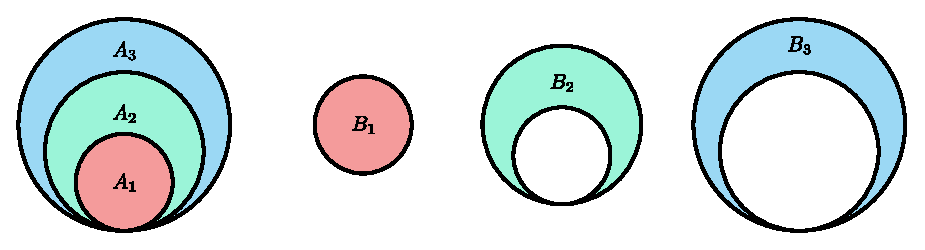
\includegraphics[width=\textwidth]{chap1/c1q1.eps}
\end{center}
Now, let \(\omega \in B_{i}\). We must have \(\omega \notin B_{j}\), since \(\omega \notin B_{i}\) is a condition for membership in \(B_{j}\). Thus \(B_{i} \cap B_{j} = \varnothing \), and each of the \(B\)'s are pairwise disjoint. 
Since \(A_{1} \subset \cdots \subset A_{n}\), we have
\[
	A_{n} = \bigcup_{i=1}^{n} A_{i} 
\]
Now consider \(\bigcup_{i=1}^{n} A_{i} \). Let \(\omega \in A_{n}\). Then \(\omega \in B_{n}\) implies \(\omega \in \bigcup_{i=1}^{n} B_{n} \). Conversely, let \(\omega \in \bigcup_{i=1}^{n} B_{n} \). Then \(\omega \in B_{i}\) for some \(i\), meaning we must have \(\omega \in A_{i}\); with \(A_{i} \subset A_{n}\), we must have \(\omega \in A_{n}\). Ergo, \(A_{n} = \bigcup_{i=1}^{n} B_{n}\).

We now have established
\[
	A_{n} = \bigcup_{i=1}^{n} A_{n} = \bigcup_{i=1}^{n} B_{n}
\]
and can conclude
\[
	\lim_{n \to \infty} A_{n} = \lim_{n \to \infty} \bigcup_{i=1}^{n} A_{n} = \lim_{n \to \infty} \bigcup_{i=1}^{n} B_{n} = A    
\]
By Kolmogorov Axiom 3 and the disjointness of the \(B\)'s, it follows that
\[
	P(A_{n}) = P\left( \bigcup_{i=1}^{n} B_{i}  \right) = \sum_{i=1}^{n} P(B_{i})	
\]
leaving the final step of taking the limits
\[
	\lim_{n \to \infty} P(A_{n}) = \lim_{n \to \infty} \sum_{i=1}^n P(B_{i}) = \sum_{i=1}^{\infty} P(B_{i}) =  P\left( \bigcup_{i=1}^{\infty} B_{i}  \right) = P(A)
\]
\textbf{Monotone Decreasing Case.} With \(A_{n}\) monotone decreasing so that \(A_{1} \supset A_{2} \supset \cdots \), let \(A = \lim_{n \to \infty} A_{n} = \bigcap_{i=1}^{\infty} A_{i}  \). By de Morgan's laws, we have
\[
	\left( \bigcap_{i=1}^{\infty} A_{i} \right)^{c} = \bigcup_{i=1}^{\infty} A_{i}^{c} 
\]
and when applied to the monotone increasing case,
\[
	\lim_{n \to \infty} P(A_{n}^{c}) = 1 - \lim_{n \to \infty} P(A_{n}) =  P \left( \bigcup_{i=1}^{\infty} A_{i}^{c} \right) = P(A^{c}) = 1 - P(A)  
\]

we can conclude
\[
	1 - \lim_{n \to \infty} P(A_{n}) = 1 - P(A) \implies \lim_{n \to \infty} P(A_{n}) = P(A) 
\]
\end{proof}

% QUESTION 2
\newpage
\qs{1.10.2}{Prove the statements in equation 1.1.}
\prp{(Wasserman Eq. 1.1)}{
	\begin{center}
	\begin{tabular}{r c l}
	$\Prob(\varnothing)$  &$=$ &$0$ \\
	$A \subset B$ &$\implies$ &$\Prob(A) \le \Prob(B)$ \\
	$0 \le$ &$\Prob(A)$ &$\le 1$ \\
	$\Prob(A^{c})$ &$=$ &$1 - \Prob(A)$ \\
	$A \bigcap B = \varnothing$ &$\implies$ &$P \big( A \bigcup B \big) = \Prob(A) + \Prob(B)$  
	\end{tabular}
	\end{center}}
\begin{proof}[Proof]
Let \(A, B\) be events. \\
\underline{$\Prob(\varnothing) = 0$} \\
We know that $\Omega^{c} = \varnothing$. Then $\Omega^{c} \cap \Omega = \varnothing$ and $\Omega^{c} \cup \Omega = \Omega$. Combining Kolmogorov Axioms 2 and 3, conclude $\Prob(\Omega) = \Prob(\Omega^{c}) + \Prob(\Omega) = \Prob(\varnothing) + \Prob(\Omega) = 1$. Another application of Axiom 2 yields $\Prob(\varnothing) = 1 - \Prob(\Omega) = 1 - 1 = 0$.

\underline{$A \subset B \implies \Prob(A) \le \Prob(B)$} \\
Consider \(A\) and \(B-A\). We have \(A \cap B-A = \varnothing\), as \(\omega \in A\) implies \(\omega \not\in B-A\) and \(\omega \in B-A\) implies \(\omega \not\in A\). 

Now we prove \(B = A \cup B-A\). If \(\omega \in A \cup B-A\) either \(\omega \in A\) or \(\omega \in B-A\). If \(\omega \in A\), then since \(A \subset B\), we have \(\omega \in B\). If \(\omega \in B-A\), then \(\omega \in B\). And if \(\omega \in B\), then \(\omega \in B-A\) implies \(\omega \in A \cup B-A\). Thus \(B = A \cup B-A\).

By Axiom 3,
\[
	\Prob(B) = \Prob(A \cup B-A) = \Prob(A) + \Prob(B-A)
\]
since \(\Prob(B-A) \ge 0\), this implies \(\Prob(A) \le \Prob(B)\).

\underline{\(0 \le \Prob(A) \le 1\)} \\
By Axiom 1, \(\Prob(A) \ge 0\). By Axioms 2 and 3, \(\Prob(\Omega) = 1 \). Then \(\Omega = A \cup A^{c}\) and \(A \cap A^{c} = \varnothing\), which in turn implies \(\Prob(\Omega) = \Prob(A) + \Prob(A^{c}) = 1\). Since \(\Prob(A^{c}) \ge 0\), we have \(\Prob(A) \le 1\). Thus \(0 \le \Prob(A) \le 1\).

\underline{\(\Prob(A^{c}) = 1 - \Prob(A)\)} \\
Since \(A^{c} \cap A = \varnothing\) and \(A^{c} \cup A = \Omega\), by Axioms 2 and 3, we have \(\Prob(\Omega) = 1 = \Prob(A) + \Prob(A^{c})\). We conclude that \(\Prob(A^{c}) = 1 - \Prob(A)\).

\underline{\(A \cap B = \varnothing \implies \Prob(A \cup B) = \Prob(A) + \Prob(B)\)} \\
By disjointness of \(A,B\), by Axiom 3, \(\Prob(A \cup B) = \Prob(A) + \Prob(B)\).
\end{proof}

\newpage
% QUESTION 3
\qs{1.10.3}{Let \(\Omega\) be a sample space and let \(A_{1}, A_{2}, \dots,\) be events. Define \(B_{n} = \bigcup_{i= n}^{\infty} A_{i} \) and \(C_{n} = \bigcap_{i=n}^{\infty} A_{i} \).
	\begin{enumerate}[label=(\alph*)]
		\item Show that \(B_{1} \supset B_{2} \supset \cdots\) and that \(C_{1} \subset C_{2} \subset \cdots\).
		\item Show that \(\omega \in \bigcap_{n=1}^{\infty} B_{n}\) if and only if \(\omega\) belongs to an infinite number of the events \(A_{1}, A_{2}, \dots\).
		\item Show that \(\omega \in \bigcup_{n=1}^{\infty} C_{n}\) if and only if \(\omega\) belongs to all the events \(A_{1}, A_{2}, \dots\) except possibly a finite number of those events.
	\end{enumerate}
}
\begin{proof}[Proof] 
	(a) For the base case, we prove \(B_{1} \supset B_{2}\). If \(\omega \in  B_{2} = \bigcup_{i=2}^{\infty} A_{i} \), then \(\omega \in A_{1} \cup \bigcup_{i=2}^{\infty} A_{i} = B_{1}\). Thus \(B_{1} \supset B_{2}.\)

Now assume \(B_{1} \supset \cdots \supset B_{n} \) is true. We want to prove that \(B_{1} \supset \cdots \supset B_{n} \supset B_{n+1}\). It will suffice to show \(B_{n} \supset B_{n+1}\). If \(\omega \in B_{n+1} = \bigcup_{i = n+1}^{\infty} A_{i} \), then we have \(\omega \in  A_{n} \cup \bigcup_{i = n+1}^{\infty} A_{i} = B_{n} \), so \(B_{n} \supset B_{n+1}\).

The proof for the \(C_{n}\)'s is analogous. For the base case, \(C_{1} \subset C_{2}\), if \(\omega \in C_{1} = \bigcap_{i=1}^{\infty} A_{i} \) then \(\omega \in A_{i}\) for all \(i\). Then we must have \(\omega \in A_{2}, A_{3}, \dots\), and consequently, \(\omega \in C_{2} = \bigcap_{i=2}^{\infty} A_{2} \).

For the induction hypothesis, suppose that \(C_{1} \subset \cdots \subset C_{n}	\). We must show \(C_{n} \subset C_{n+1}\). If \(\omega \in C_{n} = \bigcap_{i=n}^{\infty} A_{i} \), then we have \(\omega \in A_{n+1},\dots\) implying \(\omega \in C_{n+1} = \bigcap_{i=n+1}^{\infty} A_{n} \).
\vspace{12pt}
\par (b) \((\implies)\) Let \(\omega \in \bigcap_{n=1}^{\infty} B_{n} \). Suppose \(\omega\) belongs only to a finite number of events \(A_{i}\). Pick the \(A_{i}\) with the highest subscript \(i\). Now consider \(B_{i+1} = \bigcup_{j = i+1}^{\infty} A_{j} \). Our assumption of finitude implies \(\omega \not\in B_{i+1}\), a contradiction. We will come to this contradiciton for any choice of \(A_{i}\). Thus it must be that \(\omega\) belogns to an infinite number of events \(A_{i}\).

\(( \impliedby )\) Now suppose \(\omega\) belongs to an infinite number of events \(A_{i}\). We must show that \(\omega \in \bigcap_{n=1}^{\infty} B_{n}\).

For \(n=1\), we must have \(\omega \in  B_{1}\), as \(\omega\) is in infinitely many \(A_{i}\)'s, and \(B_{1} = \bigcup_{i=1}^{\infty} A_{i} \). 

Now suppose \(\omega \in B_{n} = \bigcup_{i=n}^{\infty} A_{i}\). To demonstrate \(\omega \in B_{n+1}\), we realize that we cannot have only \(\omega \in A_{n}, \omega \not\in A_{n+1}\), \dots as this would contradict the infinitude of membership. Thus we must have membership in \(A_{i}\)'s with \(i > n\). Ergo, \(\omega \in B_{n+1}\).

By induction, \(\omega \in B_{i}\) for all \(i\). Thus \(\omega \in \bigcap_{n=1}^{\infty} B_{n} \). 
\vspace{12pt}
\par (c) \(( \implies ) \) Let \(\omega \in \bigcup_{n=1}^{\infty} C_{n} \). Then \(\omega \in C_{n} = \bigcap_{i=n}^{\infty} A_{i} \) for at least one \(n\). If \(\omega \in C_{1} = \bigcap_{i=1}^{\infty} A_{i} \), then \(\omega\) belongs to all events \(A_{1}, A_{2},\dots\). Suppose otherwise that \(\omega \in  C_{n}\) for \(n \neq 1 \). Then \(\omega\) lacks membership in at least one of the \(A_{1},\dots, A_{n+1}\); in other words, it lacks membership in a finite number of those events.

\(( \impliedby )\) Let \(\omega\) belong to all \(A_{1}, A_{2}, \dots\) or otherwise lack membership in a finite number of \(A_{i}\). In the first case, \(\omega \in \bigcap_{i=1}^{\infty} A_{i} = C_{1} \) implies \(\omega \in \bigcup_{n=1}^{\infty} C_{n} \). Otherwise, pick the \(A_{i}\) with \(\omega \not\in A_{i}\) and the highest \(i\). Then we have \(\omega \in \bigcap_{j = i+1}^{\infty} A_{j} = C_{i+1} \), and still \(\omega \in \bigcup_{n = i+1}^{\infty} C_{n} \).
\end{proof}

% QUESTION 4
\qs{1.10.4}{Let \(\left\{\, A_{i} \colon i \in I \,\right\}\) be a collection of events where \(I\) is an arbitrary index set. Show that
\[
	\left( \bigcup_{i \in  I} A_{i}  \right)^{c} = \bigcap_{i \in  I} A_{i}^{c} \quad \text{and} \quad \left(\bigcap_{i \in I} A_{i} \right)^{c} = \bigcup_{i \in  I} A_{i}^{c} 
\]
Hint: First prove this for \(I = \{1, \dots, n \}\).
}

\begin{proof}[Proof]
These are the famous De Morgan's Laws.
\vspace{12pt}
\par (1) Let \(\omega \in \big(\bigcup_{i \in  I} A_{i} \big)^{c} \). Suppose \(I = \{1, \dots, n \} \). Then we have \(\omega \not\in \bigcup_{i \in  I} A_{i}\), with the following chain of implications: \(\omega \not\in A_{1}, \dots, A_{n}\) to \(\omega \in A_{1}^{c}, \dots, A_{n}^{c}\) to \(\omega \in \bigcap_{i \in  I} A_{i}^{c}\). Conversely, if \(\omega \in \bigcap_{i \in  I} A_{i}^{c}\), we must have \(\omega \not\in A_{1},\dots, A_{n}\), implying \(\omega \not\in \bigcup_{i \in  I} A_{i}\), allowing us to conclude \(\omega \in \big(\bigcup_{i \in  I} A_{i} \big)^{c} \).

That is the finite case. Suppose now that we prove the infinite case. In the base case, trivially \(\omega \in A_{1}^{c}\) implies itself. If we assume it holds for \(n-1 \  A_{i}\)'s, apply the proof for the \(n \  A_{i}\)'s to prove the infinite case by induction.
\vspace{12pt}
\par (2) Let \(\omega \in \big(\bigcap_{i \in  I} A_{i} \big)^{c}\) for \(i \in \{1, \dots, n \} \). Then \(\omega \not\in \bigcap_{i \in  I} A_{i}\), meaning \(\omega\) is bereft of membership for at least one \(A_{i}\). It follows that \(\omega \in A_{i}^{c}\), implying \(\omega \in \bigcup_{i \in  I} A_{i}^{c}\). Now suppose \(\omega \in \bigcup_{i \in  I} A_{i}^{c}\). Then \(\omega \in A_{i}^{c}\) for at least one \(i\). If so, we cannot have \(\omega \in \bigcap_{i \in  I} A_{i}\), so it must follow that \(\omega \in \big(\bigcap_{i \in  I} A_{i} \big)^{c}\). Thus \( \big(\bigcap_{i \in  I} A_{i} \big)^{c} = \bigcup_{i \in  I} A_{i}^{c}\).
\end{proof}

% QUESTION 5
\qs{1.10.5}{Suppose we toss a fair coin until we get exactly two heads. Describe the sample space \(S\). What is the probability that exactly \(k\) tosses are required?}

Descriptively, the sample space \(S\) is the set of events where the first head appears on any one of the \(1,\dots, k-1\)-th toss. In general, the probability that exactly \(k\) tosses are needed is

\[
	\Prob(k \text{ tosses}) = (k-1)(1/2)^{k}
\]
The reasoning is that since the second head is fixed on the \(k\)-th toss, there are \(k-1\) tosses for the first head to be flipped. We simulate the coin toss experiment below:

\begin{python}
def cointoss(): 
    tosses, heads = [], 0
    while (heads < 2):
        flip = random.randint(0,1)
        if (flip == 0):
            tosses.append('Heads')
            heads = tosses.count('Heads')
        else:
            tosses.append('Tails')
    return len(tosses)

def empirical(n): 
    numtosses, probs = [], []
    for i in range(0,n):
        numtosses.append(cointoss())
    for x in np.unique(numtosses): 
        probs.append((x, numtosses.count(x)/n))
    return probs

def theoretical(): 
    probs = []
    for i in range(2,24):
        probs.append((i, (i-1)*(0.5)**i))
    return probs

n = 5000
\end{python}

\begin{center}
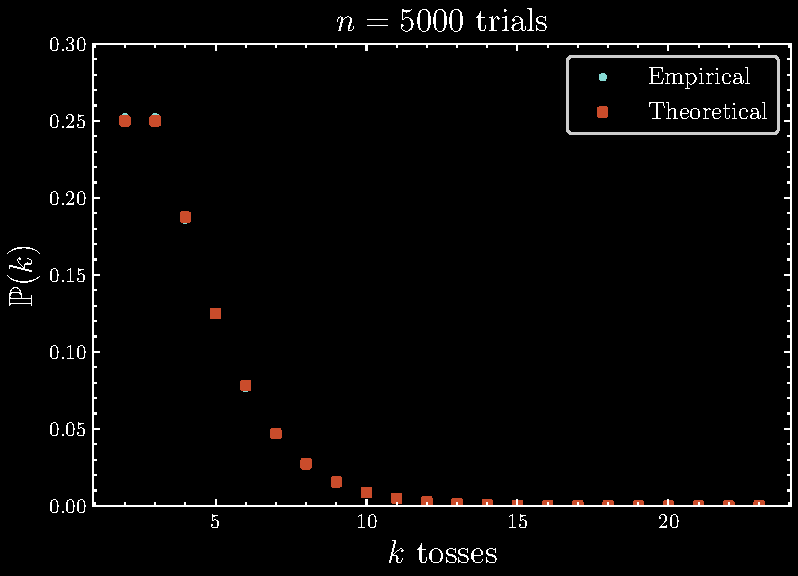
\includegraphics[width=1.0\textwidth]{chap1/chap1ex5.eps}
\end{center}

When we simulate the experiment for a large number of trials, we can see that the empirical results are quite close to the expected theoretical outcomes.

\newpage
% QUESTION 6
\qs{1.10.6}{Let \(\Omega = \{0, 1, \dots, \} \). Prove that there does not exist a uniform distribution on \(\Omega\) (i.e., if \(\Prob(A) = \Prob(B)\) whenever \(\abs{A} = \abs{B}\), then \(\Prob\) cannot satisfy the axioms of probability).}

\begin{proof}[Proof] 
	Suppose that \(\Omega\) has a uniform distribution, and \(\Prob(A) = \Prob(B)\) whenever \(\abs{A} = \abs{B}\). Consider the disjoint singletons \(\{0\}, \{1\}, \dots\). By Axiom 3, we have
	\[
	\Prob\left(\bigcup_{k=0}^{\infty} \{k\} \right) = \sum_{k=0}^{\infty} \Prob(\{k\})
	\]
However,
\[
	\bigcup_{k=0}^{\infty} \{k\} = \Omega 
\]
which from Axiom 2 implies
\[
	\Prob\left(\bigcup_{k=0}^{\infty} \{k\} \right) = \Prob(\Omega) = 1
\]
But by our uniform distribution assumption, each constituent of the sum of singleton probabilities is zero (picking a particular integer out of infinite possibilities is effectively zero probability). Thus we must have
\[
	\sum_{k=0}^{\infty} \Prob(\{k\}) = 0
\]
But \(\Prob\big(\bigcup_{k=0}^{\infty} \{k\} \big) = 1 \), a contradiction.
\end{proof}

% QUESTION 7
\qs{1.10.7}{Let \(A_{1}, A_{2},\dots\) be events. Show that
\[
	\Prob\left(\bigcup_{n=1}^{\infty} A_{n} \right) \le \sum_{n=1}^{\infty} \Prob(A_{n}).
\]
Hint: Define \(B_{n} = A_{n} - \bigcup_{i=1}^{n-1} A_{i} \). Then show that the \(B_{n}\) are disjoint and that \(\bigcup_{n=1}^{\infty} A_{n} = \bigcup_{n=1}^{\infty} B_{n} \). 
}
\begin{proof}[Proof] 
	Define \(B_{n} = A_{n} - \bigcup_{i=1}^{n-1} A_{i} \). First we prove the \(B_{n}\) are disjoint. Take \(B_{k}, B_{j}\) for \(k \neq j\). Without loss of generality, suppose \(k < j\). Let \(\omega \in B_{k}\). Then \(\omega \in A_{k} - \bigcup_{i=1}^{k-1} A_{i} \); importantly, \(\omega \in A_{k}\). Then we must have \(\omega \in \bigcup_{i=1}^{j-1} A_{i} \), implying \(\omega \not\in A_{j} - \bigcup_{i=1}^{j-1} A_{i} = B_{j} \).

	Conversely, if \(\omega \in B_{j} = A_{j} - \bigcup_{i=1}^{j-1} A_{i} \), we must have \(\omega \not\in \bigcup_{i=1}^{j-1} A_{i}\). Then we have \(\omega \not\in A_{k}\), implying \(\omega \not\in A_{k} - \bigcup_{i=1}^{k-1} A_{i} \). Thus \(B_{i} \cap B_{j} = \varnothing\) and \(B_{i}, B_{j}\) are disjoint.

	Now, we establish \(\bigcup_{n=1}^{\infty} A_{n} = \bigcup_{n=1}^{\infty} B_{n} \). Let \(\omega \in \bigcup_{n=1}^{\infty} \). Then \(\omega \in A_{k}\) for some \(k\)('s). Choose the \(A_{k}\) with the lowest \(k\). Then \(\omega \in A_{k} - \bigcup_{i=1}^{k-1} A_{i} = B_{k} \) implies \(\omega \in \bigcup_{n=1}^{\infty} B_{n} \).

	Conversely, let \(\omega \in \bigcup_{n=1}^{\infty} B_{n} \). Then \(\omega \in B_{k} = A_{k} - \bigcup_{i=1}^{k=1} A_{i} \) for some \(k\)('s). Then \(\omega \in A_{k}\) implies \(\omega \in \bigcup_{n=1}^{\infty} A_{n} \). Thus \(\bigcup_{n=1}^{\infty} A_{n} = \bigcup_{n=1}^{\infty} B_{n}  \).

	By Axiom 3 and the disjointness of \(B_{n}\), we have
\[
	\Prob\left(\bigcup_{n=1}^{\infty} B_{n} \right) = \sum_{n=1}^{\infty} \Prob(B_{n})
\]
Since \(B_{n} = A_{n} - \bigcup_{i=1}^{n-1} A_{i} \subset A_{n} \), we have \(\Prob(B_{n}) \le \Prob(A_{n})\) for all \(n\). Then \(\sum_{n=1}^{\infty} \Prob(B_{n}) \le \sum_{n=1}^{\infty} \Prob(A_{n})\). At last we may conclude
\[
	\Prob\left(\bigcup_{n=1}^{\infty} A_{n}  \right) \le \sum_{n=1}^{\infty} \Prob(A_{n})
\]
\end{proof}

% QUESTION 8
\qs{1.10.8}{Suppose that \(\Prob(A_{i}) = 1\) for each \(i\). Prove that
\[
	\Prob\left(\bigcap_{i=1}^{\infty}A_{i} \right) = 1
\]
}

\begin{proof}[Proof] 
	By premise, \(\Prob(A_{i} = 1)\) implies \(\Prob(A_{i}^{c}) = 1 - \Prob(A_{i}) = 0\). Now, since \(A_{1}^{c}, A_{2}^{c},\dots\) all have probability zero, it must be the case that \(\Prob(\bigcup_{i=1}^{\infty}A_{i}^{c} ) = 0\). By De Morgan's laws,
\[
	\Prob\left(\bigcup_{i=1}^{\infty} A_{i}^{c} \right) = \Prob\left( \left(\bigcap_{i=1}^{\infty} A_{i} \right)^{c} \right) = 0 
\]
Allowing us to conclude
\[
	\Prob\left( \bigcap_{i=1}^{\infty} A_{i} \right) = 1 - \Prob\left( \left(\bigcap_{i=1}^{\infty} A_{i} \right)^{c} \right) = 1 
\]
\end{proof}

% QUESTION 9
\qs{1.10.9}{For fixed \(B\) such that \(\Prob(B) > 0\), show that \(\Prob(\cdot \mid B)\) satifies the axioms of probability.}

\begin{proof}[Proof] 
(i) For independent \(\cdot, B\), we have \(\Prob(\cdot B) = \Prob(\cdot) \Prob(B)\), and if \(\Prob(\cdot) \ge 0\) then \(\Prob(\cdot \mid B) = \Prob(\cdot) \ge 0\). Otherwise, \(\Prob(\cdot B), \Prob(B) \ge 0\) implies \(\Prob(\cdot \mid B) \ge 0\).
\vspace{12pt}
\par (ii) If \(\cdot = \Omega\), then
\[
	\Prob(\Omega \mid B) = \frac{\Prob(\Omega B)}{\Prob(B)} = \frac{\Prob(\Omega) \Prob(B)}{\Prob(B)} = \Prob(\Omega) = 1
\]
\vspace{12pt}
\par (iii) If \(A_{i} \cap A_{j} = \varnothing\), then \( (A_{i} \cap B) \cap (A_{j} \cap B) = \varnothing\). Then we have

\begin{align*}
	\Prob(A_{i} \cup A_{j} \mid B) & = \frac{\Prob((A_{i} \cup A_{j}) \cap B)}{\Prob(B)} \\
			       & = \frac{\Prob((A_{i} \cap B) \cup (A_{j} \cap B))}{\Prob(B)}  \\
			       & = \frac{\Prob(A_{i} \cap B) + \Prob(A_{j} \cap B)}{\Prob(B)} \\
			       & = \Prob(A_{i} \mid B) + \Prob(A_{j} \mid B)
\end{align*}

To generalize for infinitely many disjoint events \(A_{i}\), observe that 
\[
	\left( \bigcup_{i = 1}^{\infty} A_{i} \right) \cap B = \bigcup_{i = 1}^{\infty} (A_{i} \cap B)
\]
Applying the logic for the case with two disjoint events, we can immediately conclude
\[
	\Prob\left( \bigcup_{i = 1}^{\infty} A_{i} \Bigg| B \right) = \sum_{i=1}^{\infty} \Prob(A_{i} \mid B)
\]
\end{proof}

\newpage
% QUESTION 10
\qs{1.10.10}{You have probably heard it before. Now you can solve it rigorously. It is called the "Monty Hall Problem." A prize is placed at random behind one of three doors. You pick a door. To be concrete, let's suppose you always pick door 1. Now Monty Hall chooses one of the other two doors, opens it and shows you that it is empty. He then gives you the opportunity to keep your door or switch to the other unopened door. Should you stay or switch? Intuition suggests it doesn't matter. The correct answer is you should switch. Prove it. It will  help to specify the sample space and the relevant events carefully. Thus write \(\Omega = \left\{\, (\omega_{1}, \omega_{2}) \colon \omega_{i} \in \{1,2,3 \} \,\right\}\) where \(\omega_{1}\) is where the prize is and \(\omega_{2}\) is the door Monty opens. }

There are some insights we should be aware of. Firstly, there is equal chance of the prize appearing behind any one of the three doors, i.e., \(\Prob(\text{Prize, Door } i) = 1/3\). Secondly, the choice of door for Monty Hall \textit{depends on our choice of door}. Our pick of door also follows equal probability for each door, or \(1/3\).

Using Bayes' Theorem, without loss of generality, suppose you pick door 1, the prize lies behind door 2, and Monty Hall picks door 3. We wish to find the probability that the prize is behind door 2, \textit{given that Monty Hall opens door 3}.
\begin{align*}
	\Prob(\text{Prize, Door }2 \mid \text{Monty, Door }3) & = \frac{\Prob(\text{M, D }3 \mid \text{P, D } 2)\Prob(\text{P, D }2)}{\sum \Prob(\text{M, D } 3 \mid \text{P, D } i)\Prob(\text{P, D } i)} \\
	 & = \frac{1 \cdot 1/3}{1 \cdot 1/3 + 1/2 \cdot 1/3 + 0 \cdot 1/3} \\
	 & = \boxed{2/3}
\end{align*}

Here, it is advantageous to switch doors, as the prior probability \((1/3)\) changes to the posterior probability \((2/3)\) once Monty Hall diverges additional information that his door is empty.

It is useful to illustrate the sample space by way of a probability tree:

\begin{center}
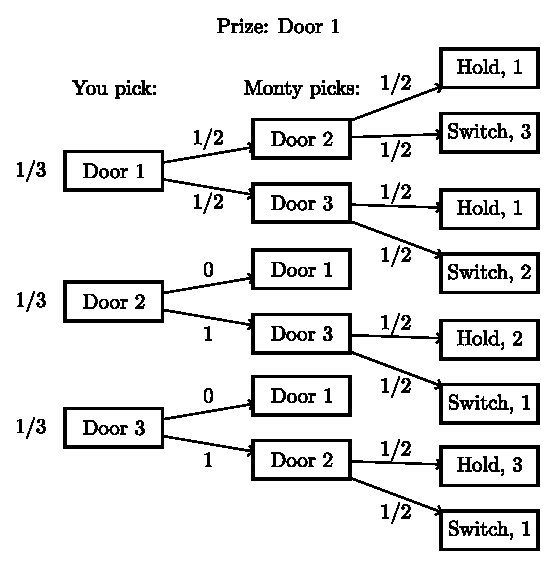
\includegraphics[width=1.0\textwidth]{chap1/c1q10.eps}
\end{center}

Assuming without loss of generality that the prize lies behind door 1, we can calculate the conditional probabilities of winning given that we either hold or switch. 

Let \(Y\) be your choice of door and \(M\) be Monty Hall's. Moreover, let \(\alpha\) be
\begin{align*}
	\alpha & = \Prob(Y=1)\Prob(M=2 \mid Y=1)\Prob(\text{Hold }1 \mid M = 2) \\ 
	 & \quad + \Prob(Y=1)\Prob(M=3 \mid Y=1)\Prob(\text{Hold }1 \mid M=3) \\
	 & \quad + \Prob(Y=2)\Prob(M=3 \mid Y=2)\Prob(\text{Hold }2 \mid M=3) \\
	 & \quad + \Prob(Y=3)\Prob(M=2 \mid Y=3)\Prob(\text{Hold } 3 \mid M=2) \\
	 & = 1/3 \cdot 1/2 \cdot 1/2 + 1/3 \cdot 1/2 \cdot 1/2 + 1/3 \cdot 1/2 + 1/3 \cdot 1/2 \\
	 & = 1/2
\end{align*}

We calculate
\begin{align*}
	\Prob(\text{Win } \mid \text{ Hold}) & = \frac{\Prob(Y=1)\Prob(M=2 \mid Y=1)\Prob(\text{Hold } 1 \mid M=2)}{\alpha} \\
	 & \quad + \frac{\Prob(Y=1)\Prob(M=3 \mid Y=1)\Prob(\text{Hold }1 \mid M=3)}{\alpha} \\
	 & = \frac{1/3 \cdot 1/2 \cdot 1/2 + 1/3 \cdot 1/2 \cdot 1/2}{1/2} \\
	 & = \boxed{1/3}
\end{align*}

An analogous calculation for the switching conditional probability gives us
\[
	\Prob(\text{Win } \mid \text{ Switch}) = \boxed{2/3}
\]
Lastly, there is a famous anecdote of Erd{\"o}s refusing to accept the result of the Monty Hall problem until examining a simulation of the game. You may find yourself burdened by a similar sentiment. Indeed, the experimental result aligns with our derivations above:

\begin{python}
def montyhallswitch(): 
    doors = list(range(2, 4))
    prizedoor = random.randint(1,3)
    if (prizedoor == 2 or prizedoor == 3): 
        montydoors = [x for x in doors if x != prizedoor]
        montypicks = montydoors[0]
    else:
        montypicks = random.randint(2,3) 
    doors.remove(montypicks)
    yourswitch = doors[0]
    return(prizedoor == yourswitch)

def montyhallhold(): 
    prizedoor = random.randint(1,3)
    return(prizedoor == 1)

def iterationswitch(n): 
    runs = []
    for i in range(1,n+1):
        runs.append(montyhallswitch())
    probs = runs.count(True)/(n+1)
    return probs

def iterationhold(n): 
    runs = []
    for i in range(1,n+1):
        runs.append(montyhallhold())
    probs = runs.count(True)/(n+1)
    return probs

n = 5000
trials = list(range(10, n+1, 5)) 
switchprob, holdprob = [], []
for i in trials: 
    switchprob.append(iterationswitch(i))
    holdprob.append(iterationhold(i))
\end{python}

\begin{center}
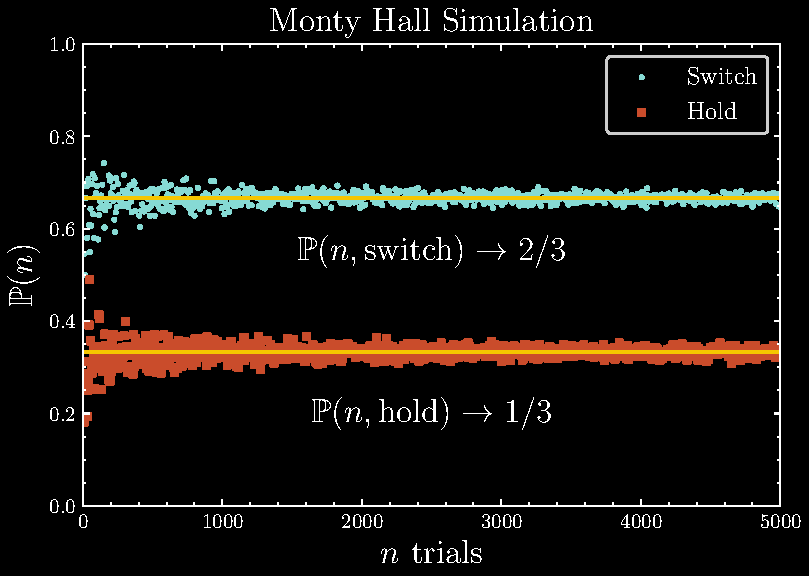
\includegraphics[width=1.0\textwidth]{chap1/chap1ex10.eps}
\end{center}

% QUESTION 11
\qs{1.10.11}{Suppose that \(A\) and \(B\) are independent events. Show that \(A^{c}\) and \(B^{c}\) are independent events.}

\begin{proof}[Proof] 
By premise, \(\Prob(AB) = \Prob(A)\Prob(B)\). We have \(\Prob(A^{c}) = 1 - \Prob(A)\) and \(\Prob(B^{c}) = 1 - \Prob(B)\). To find \(\Prob(A^{c} B ^{c})\), we observe these disjoint events:

\begin{align*}
	\Prob(A-B) & = \Prob(A) - \Prob(AB) \\
	\Prob(B-A) & = \Prob(B) - \Prob(AB) \\
	           & \Prob(AB) \\
		   & \Prob(A^{c}B^{c})
\end{align*}

Thus we have
\[
	1 = \Prob(A-B) + \Prob(B-A) + \Prob(AB) + \Prob(A^{c}B^{c})
\]
which implies
\begin{align*}
	\Prob(A^{c}B^{c}) & = 1 - \Prob(A-B) - \Prob(B-A) - \Prob(AB) \\
	 & = 1 - (\Prob(A) - \Prob(AB)) - (\Prob(B) - \Prob(AB)) - \Prob(AB) \\
	 & = 1 - \Prob(A) - \Prob(B) + \Prob(AB)
\end{align*}
Now calculate
\begin{align*}
	\Prob(A^{c})\Prob(B^{c}) & = (1 - \Prob(A))(1 - \Prob(B)) \\
	 & = 1 - \Prob(A) - \Prob(B) + \Prob(A)\Prob(B) \\
	 & = 1 - \Prob(A) - \Prob(B) + \Prob(AB)
\end{align*}
Thus \(\Prob(A^{c}B^{c}) = \Prob(A^{c})\Prob(B^{c})\), and \(A^{c}\) and \(B^{c}\) are independent.
\end{proof}

% QUESTION 12
\qs{1.10.12}{There are three cards. The first is green on both sides, the second is red on both sides and the third is green on one side and red on the other. We choose a card at random and we see one side (also chosen at random). If the side we see is green, what is the probability that the other side is also green? Many people intuitively answer \(1/2\). Show that the correct answer is \(2/3\).}
\begin{proof}[Proof] 
Let \(GG, RR, GR\) correspond to the first, second, and third cards. Using Bayes' Theorem: we calculate the probability of having drawn a \(GG\) card given that we see \(G\), or \(GR\) given that we see \(G\). Calculate
\begin{align*}
	\Prob(GG \mid G) & = \frac{\Prob(G \mid GG) \Prob(GG)}{\Prob(G \mid GG)\Prob(GG) + \Prob(G \mid RR)\Prob(RR) + \Prob(G \mid GR)\Prob(GR)} \\
	 & = \frac{1 \cdot 1/3}{1 \cdot 1/3 + 0 \cdot 1/3 + 1/2 \cdot 1/3} \\
	 & = \boxed{2/3} \\
	\Prob(GR \mid G) & = \frac{\Prob(G \mid GR)\Prob(GR)}{\Prob(G \mid GR)\Prob(GR) + \Prob(G \mid RR)\Prob(RR) + \Prob(G \mid GG)\Prob(GG)} \\
	 & = \frac{1/2 \cdot 1/3}{1/2 \cdot 1/3 + 0 \cdot 1/3 + 1 \cdot 1/3} \\
	 & = \boxed{1/3}
\end{align*}
\end{proof}

Simulating the card game, we find that the empirical outcome agrees with our theoretical result.

\begin{python}
def cardgame(): 
    first, second, third = ('G','G'), ('R','R'), ('G','R')
    mychoice = random.choice([first, second, third])
    myside = random.choice(mychoice)
    if (myside == 'G' and 'R' not in mychoice):
        return(True, True) 
    elif (myside == 'G' and 'R' in mychoice):
        return(True, False) 
    else:
        return(False, False) 
    
def iteration(n): 
    runs = []
    for i in range(1,n+1):
        runs.append(cardgame())
    probs = runs.count((True, True))/
    	(runs.count((True, True)) + runs.count((True, False)))
    return probs

n=2500
games = list(range(10, n+1))
cardprob = []
for i in games: 
    cardprob.append(iteration(i))
\end{python}
\begin{center}
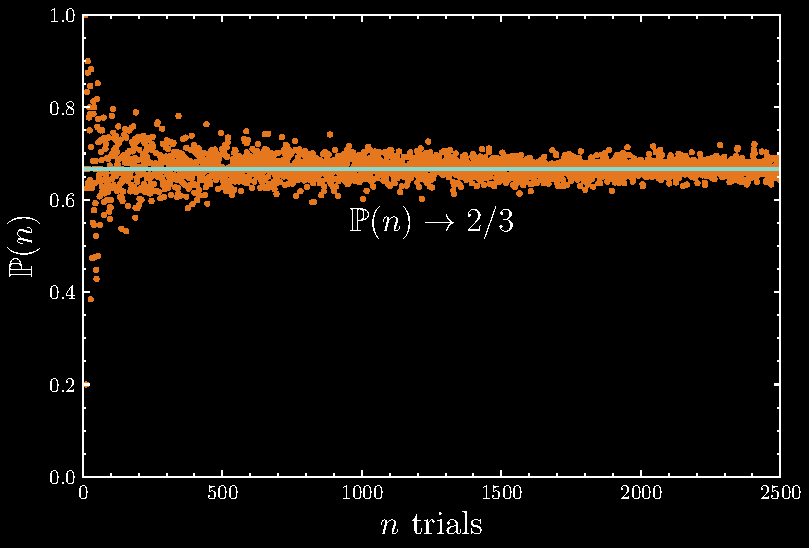
\includegraphics[width=1.0\textwidth]{chap1/chap1ex12}
\end{center}

% QUESTION 13
\qs{1.10.13}{Suppose that a fair coin is tossed repeatedly until both a head and tail have appeared at least once.
\begin{enumerate}[label=(\alph*)]
	\item Describe the sample space \(\Omega\).
	\item What is the probability that three tosses will be required?
\end{enumerate}}

(a) The sample space is given by
\[
	\Omega = \{HT, HHT, \dots, \underbrace{H \cdots H}_{k}T, \dots, TH, TTH, \dots, \underbrace{T \cdots T}_{k}H, \dots \}
\]
\vspace{12pt}
\par (b) The theoretical derivation of the probability is
\begin{align*}
	\Prob(\text{3 tosses}) & = \Prob(HHT) + \Prob(TTH)  \\
	 & = (1/2)^{3} + (1/2)^{3} \\
	 & = \boxed{1/4}
\end{align*}

By simulation, we can observe the empirical probability of three tosses aligns with the theoretical result, as well as the probabilities for other numbers of tosses:

\begin{python}
def cointoss(): 
    tosses, heads, tails = [], 0, 0
    while (heads < 1 or tails < 1):
        flip = random.randint(0,1)
        if (flip == 0):
            tosses.append('Heads')
            heads = tosses.count('Heads')
        else:
            tosses.append('Tails')
            tails = tosses.count('Tails')
    return len(tosses)

def empirical(n): 
    numtosses, probs = [], []
    for i in range(0,n):
        numtosses.append(cointoss())
    for x in np.unique(numtosses): 
        probs.append((x, numtosses.count(x)/n))
    return probs

n = 5000
\end{python}
\begin{center}
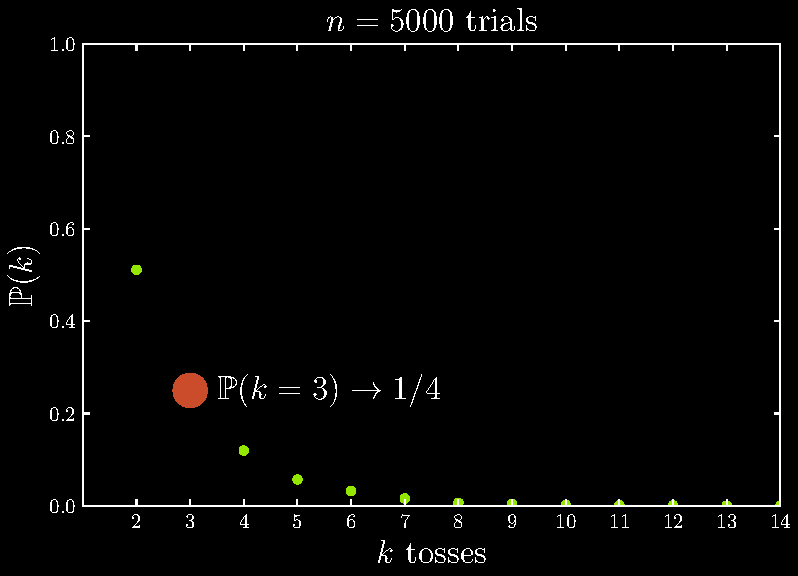
\includegraphics[width=1.0\textwidth]{chap1/chap1ex13}
\end{center}

% QUESTION 14
\qs{1.10.14}{Show that if \(\Prob(A) = 0\) or \(\Prob(A) = 1\) then \(A\) is independent of every other event. Show that if \(A\) is independent of itself then \(\Prob(A)\) is either \(0\) or \(1\).}
\begin{proof}[Proof] 
Let \(B\) be any event. Then if \(\Prob(A) = 0\), we have \(\Prob(AB) = 0\). Put differently, if \(A\) can never happen, then surely \(A\) \textit{and} \(B\) could never happen. Now, it must also be true that \(P(A)\Prob(B) = 0\), so it follows that \(\Prob(AB) = \Prob(A)\Prob(B) = 0\) and \(A\) is independent of all events.

Now suppose \(\Prob(A) = 1\). Then \(\Prob(AB) = \Prob(B)\). The reasoning is that since \(A\) will \textit{always} happen, whether \(A\) and \(B\) happen together is contingent on \(B\) happening. Thus we can write \(\Prob(AB) = \Prob(A)\Prob(B) = \Prob(B)\), again proving independence of A relative to all other events.

Lastly, suppose \(A\) is independent of itself. Then \(\Prob(AA) = \Prob(A) = \Prob(A)\Prob(A)\), implying \(\Prob(A) = 0\) or \(\Prob(A) = 1\).
\end{proof}

\newpage
% QUESTION 15
\qs{1.10.15}{The probability that a child has blue eyes is \(1/4\). Assume independence between children. Consider a family with \(3\) children.\begin{enumerate}[label=(\alph*)]
	\item If it is known that at least one child has blue eyes, what is the probability that at least two children have blue eyes?
	\item If it is known that the youngest child has blue eyes, what is the probability that at least two children have blue eyes?
\end{enumerate}}

(a) The complement event to "at least one child has blue eyes" -- call it \(A\) -- is "no child has blue eyes." The probability that a child does not have blue eyes is \(1 - p = 3/4\). Then we have
\[
	\Prob(A) = 1 - (3/4)^{3} = 1 - 27/64 = 37/64
\]
The probability that "at least two children have blue eyes" -- call this one \(B\) -- is the sum of the mutually exclusive probabilities of either two or three children having blue eyes. This is given by
\begin{align*}
	\Prob(B) & = \Prob(\text{2 children} + \text{3 children}) \\
		 & = \binom{3}{2} (1/4)^{2} (3/4) + (1/4)^{3} \\
		 & = 9/64 + 1/64 \\
		 & = 10/64
\end{align*}
Now we can calculate the probability of at least two children having blue eyes, given that at least one child has blue eyes.
\begin{align*}
	\Prob(B \mid A) & = \frac{\Prob(BA)}{\Prob(A)} \\
	 & = (10/64)(64/37) \\
	 & = \boxed{10/37}
\end{align*}
\par (b) The probability that the youngest child has blue eyes (call it C) is \(1/4\). Let \(D\) be the event that at least two children have blue eyes, with one of them being the youngest child. Then we have
\begin{align*}
	\Prob(D) & = 2(1/4)^{2}(3/4) + (1/4)^{3} \\
	 & = 6/64 + 1/64 \\
         & = 7/64
\end{align*}
Lastly, the probability that at least two children have blue eyes given that the youngest child is known to have blue eyes is
\begin{align*}
	\Prob(D \mid C) & = \frac{\Prob(DC)}{\Prob(C)} \\
	 & = \frac{7/64}{1/4} \\
	 & = \boxed{7/16}
\end{align*}

% QUESTION 16
\qs{1.10.16}{Prove Lemma 1.14.}
\lemma{(Wasserman 1.14)}{If \(A\) and \(B\) are independent events then \(\Prob(A \mid B) = \Prob(A)\). Also, for any pair of events \(A\) and \(B\),\[
	\Prob(AB) = \Prob(A \mid B)\Prob(B) = \Prob(B \mid A)\Prob(A)
\]}
\begin{proof}[Proof] 
\begin{align*}
	\Prob(A \mid B) = \frac{\Prob(AB)}{\Prob(B)} & = \frac{\Prob(A)\Prob(B)}{\Prob(B)} = \Prob(A) \\
	\Prob(A \mid B) = \frac{\Prob(AB)}{\Prob(B)} & \implies \Prob(A \mid B) \Prob(B) = \Prob(AB)  \\
	\Prob(B \mid A) = \frac{\Prob(AB)}{\Prob(A)} & \implies \Prob(B \mid A)\Prob(A) = \Prob(AB)
\end{align*}
\end{proof}

% QUESTION 17
\qs{1.10.17}{Show that
\[
	\Prob(ABC) = \Prob(A \mid BC)\Prob(B \mid C)\Prob(C)
\]}
\begin{proof}[Proof] 
\[
	\Prob(ABC) = \Prob(A  \mid  BC)\Prob(BC) = \Prob(A \mid BC)\Prob(B \mid C)\Prob(C)
\]
\end{proof}

% QUESTION 18
\qs{1.10.18}{Suppose \(k\) events form a partition of the sample space \(\Omega\), i.e., they are disjoint and \(\bigcup_{i=1}^{k} A_{i} = \Omega \). Assume that \(\Prob(B) > 0\). Prove that if \(\Prob(A_{1}  \mid  B) < \Prob(A_{1})\) then \(\Prob(A_{i}  \mid  B) > \Prob(A_{i})\) for some \(i = 2, \dots, k\).}
\begin{proof}[Proof] 
By disjointness of events, we have
\[
	\sum_{i=1}^{k} \Prob(A_{i}) = 1 \quad \text{and} \quad \sum_{i=1}^{k} \Prob(A_{i}  \mid  B) = 1
\]
with the second equality following from 1.10.9. Let \(\Prob(A_{1}  \mid  B) < \Prob(A_{1})\). It cannot be the case that we have \(\Prob(A_{i}  \mid  B) < \Prob(A_{i})\) for the remaining \(i = 2,\dots,k\), for this would violate additivity of the conditional probabilities to unity:
\[
	\sum_{i=2}^{k} \Prob(A_{i}  \mid  B) < \sum_{i=2}^{k} \Prob(A_{i}) = 1
\]
So would the condition that \(\Prob(A_{i}  \mid  B) = \Prob(A_{i})\) for the remaining \(i\). Thus at least one of the \(\Prob(A_{i}  \mid  B)\) must be greater than \(A_{i}\) for the unity sum condition to be met.
\end{proof}

% QUESTION 19
\qs{1.10.19}{Suppose that 30 percent of computer owners use a Macintosh, 50 percent use Windows, and 20 percent use Linux. Suppose that 65 percent of the Mac users have succumbed to a computer virus, 82 percent of the Windows users get the virus, and 50 percent of the Linux users get the virus. We select a person at random and learn that her system was infected with the virus. What is the probability that she is a Windows user?}

By Bayes' Theorem:
\begin{align*}
	\Prob(\text{Windows}  \mid  \text{Virus}) & = \frac{\Prob(\text{V}  \mid  \text{W})\Prob(\text{W})}{\Prob(\text{V}  \mid  \text{W})\Prob(\text{W}) + \Prob(\text{V}  \mid  \text{M})\Prob(\text{M}) + \Prob(\text{V}  \mid  \text{L})\Prob(\text{L})}  \\
	 & = \frac{0.82 \cdot 0.5}{0.82 \cdot 0.5 + 0.65 \cdot 0.3 + 0.5 \cdot 0.2} \\
	 & = \boxed{0.582}
\end{align*}

% QUESTION 20
\qs{1.10.20}{A box contains 5 coins and each has a different probability of showing heads. Let \(p_{1}, \dots, p_{5}\) denote the probability of heads on each coin. Suppose that
\[
	p_{1} = 0, p_{2} = 1/4, p_{3} = 1/2, p_{4} = 3/4 \ \text{and} \ p_{5} = 1.
\]
Let \(H\) denote "heads is obtained" and let \(C_{i}\) denote the event that coin \(i\) is selected.
\begin{enumerate}[label=(\alph*)]
	\item Select a coin at random and toss it. Suppose a head is obtained. What is the posterior probability that coin \(i\) was selected \((i = 1,\dots,5)\)? In other words, find \(\Prob(C_{i} \mid H)\) for \(i = 1,\dots,5\).
	\item Toss the coin again. What is the probability of another head? In other words find \(\Prob(H_{2} \mid H_{1})\) where \(H_{j} = \text{"heads on toss } j.\)" 

	Now suppose that the experiment was carried out as follows: We select a coin at random and toss it until a head is obtained.
	\item Find \(\Prob(C_{i} \mid B_{4})\) where \(B_{4} = \) "first head is obtained in toss 4."
\end{enumerate}
}	

Apply Bayes' Theorem for all parts.

(a) Here, \(\sum \Prob(H \mid C_{i})\Prob(C_{i}) = 1/5 \cdot \Big(\sum p_{i} \Big) = 1/5 \cdot 5/2 = 1/2 \).

\begin{align*}
	\Prob(C_{1} \mid H) & = \frac{\Prob(H \mid C_{1})\Prob(C_{1})}{\sum \Prob(H \mid C_{i})\Prob(C_{i})} = \boxed{0} \\
	\Prob(C_{2} \mid H) & = \frac{\Prob(H \mid C_{2})\Prob(C_{2})}{\sum \Prob(H \mid C_{i})\Prob(C_{i})} = \frac{1/4 \cdot 1/5}{1/2} = \boxed{1/10}  \\
	\Prob(C_{3} \mid H) & = \frac{\Prob(H \mid C_{3})\Prob(C_{3})}{\sum \Prob(H \mid C_{i})\Prob(C_{i})} = \frac{1/2 \cdot 1/5}{1/2} = \boxed{2/10} \\
	\Prob(C_{4} \mid H) & = \frac{\Prob(H \mid C_{4})\Prob(C_{4})}{\sum \Prob(H \mid C_{i})\Prob(C_{i})} = \frac{3/4 \cdot 1/5}{1/2} = \boxed{3/10} \\
	\Prob(C_{5} \mid H) & = \frac{\Prob(H \mid C_{5})\Prob(C_{5})}{\sum \Prob(H \mid C_{i})\Prob(C_{i})} = \frac{1 \cdot 1/5}{1/2} = \boxed{4/10}
\end{align*}

Empirical simulation:

\begin{python}
def coinselect():
  coin = random.randint(1,5)
  return coin

def coinprob(i):
  coinface = ['H', 'T']
  headsprob=[0, 0.25, 0.5, 0.75, 1]
  randomFace = choice( 
    coinface, 1, p=[headsprob[i-1], 1-headsprob[i-1]])
  return randomFace[0], i

def iteration(n):
  sample, probs = [], []
  for i in range(1,n):
    sample.append(coinprob(coinselect()))
  heads = len([i for i in sample if 'H' in i])
  for i in list(range(1,6)):
    probs.append(sample.count(('H',i)) / heads)
  return probs

n = 10000
\end{python}

\begin{center}
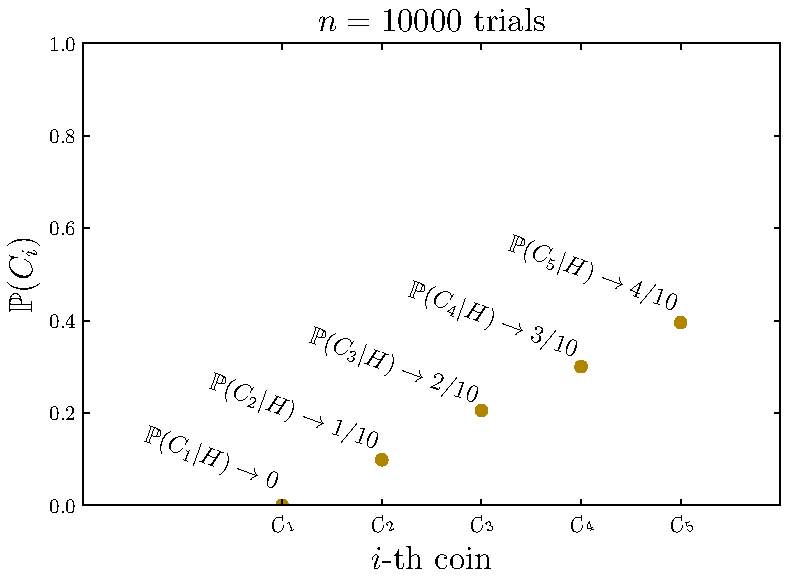
\includegraphics[width=1.0\textwidth]{chap1/chap1ex20a}
\end{center}

\par (b) By the Law of Total Probability, \(\Prob(H_{1}) = 1/5 \cdot \sum p_{i} = 1/2\). To calculate \(\Prob(H_{2} \mid H_{1})\), write
\begin{align*}
	\Prob(H_{2} \mid H_{1}) & = \frac{\Prob(H_{2}H_{1})}{\Prob(H_{1})} \\
	 & = \frac{1/5 \cdot \sum p_{i}^{2}}{1/2} \\
	 & = \frac{3/8}{1/2} \\
	 & = \boxed{3/4}
\end{align*}

Empirical simulation:

\begin{python}
def coinselect():
  coin = random.randint(1,5)
  return coin

def coinprob(i, k):
  coinface = ['H', 'T']
  headsprob=[0, 0.25, 0.5, 0.75, 1]
  randomFace = choice( 
    coinface, k, p=[headsprob[i-1], 1-headsprob[i-1]])
  return randomFace.tolist(), i

def iteration(n):
  sample, probs = [], []
  for i in range(1,n):
    sample.append(coinprob(coinselect(), k))
  firsttossheads = len(
    [i for i in sample if ['H', 'H'] in i or ['H', 'T'] in i])
  for i in range(1,6):
    probs.append(sample.count((['H','H'],i)) / firsttossheads)
  return sum(probs)

n, k, probs = 10000, 2, []

for i in range(10,n+1):
  probs.append(iteration(n))
\end{python}

\begin{center}
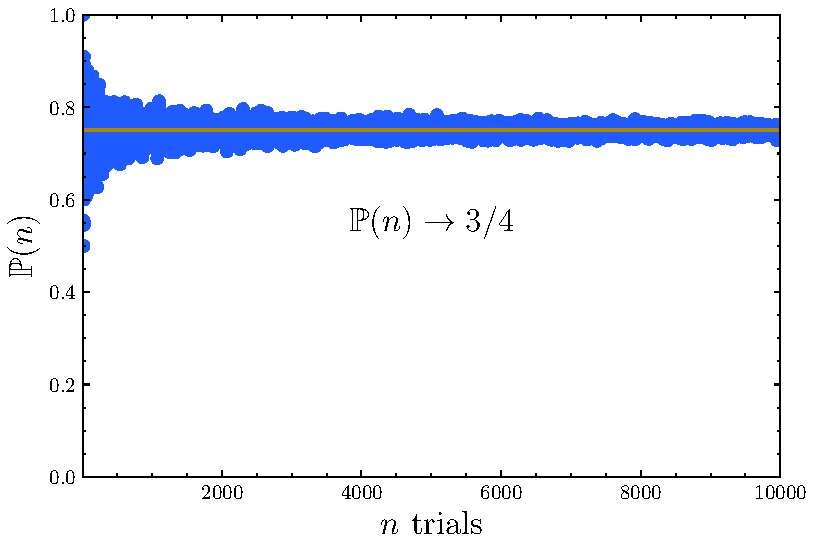
\includegraphics[width=1.0\textwidth]{chap1/chap1ex20b}
\end{center}

\par (c) Here, \(\sum \Prob(B_{4} \mid C_{i})\Prob(C_{i}) = 1/5 \cdot \sum (1-p_{i})^{3}p_{i} = 0.0359375\).

\begin{align*}
	\Prob(C_{1} \mid B_{4}) & = \frac{\Prob(B_{4} \mid C_{1})\Prob(C_{1})}{\sum \Prob(B_{4} \mid C_{i})\Prob(C_{i})} = \boxed{0}  \\
\Prob(C_{2} \mid B_{4}) & = \frac{\Prob(B_{4} \mid C_{2})\Prob(C_{2})}{\sum \Prob(B_{4} \mid C_{i})\Prob(C_{i})} = \frac{(3/4)^{3}(1/4)(1/5)}{0.0359375} = \boxed{0.587} \\
	\Prob(C_{3} \mid B_{4}) & = \frac{\Prob(B_{4} \mid C_{3})\Prob(C_{3})}{\sum \Prob(B_{4} \mid C_{i})\Prob(C_{i})} = \frac{(1/2)^{4}(1/5)}{0.0359375} = \boxed{0.348} \\
	\Prob(C_{4} \mid B_{4}) & = \frac{\Prob(B_{4} \mid C_{4})\Prob(C_{4})}{\sum \Prob(B_{4} \mid C_{i})\Prob(C_{i})} = \frac{(1/4)^{3}(3/4)(1/5)}{0.0359375} = \boxed{0.065} \\
	\Prob(C_{5} \mid B_{4}) & = \frac{\Prob(B_{4} \mid C_{5})\Prob(C_{5})}{\sum \Prob(B_{4} \mid C_{i})\Prob(C_{i})} = \boxed{0}
\end{align*}

Empirical simulation:

\begin{python}
def coinselect():
  coin = random.randint(1,5)
  return coin

def coinprob(i, k): 
  coinface = ['H', 'T']
  headsprob=[0, 0.25, 0.5, 0.75, 1]
  randomFace = choice(  
    coinface, k, p=[headsprob[i-1], 1-headsprob[i-1]])
  return randomFace.tolist(), i

def iteration(n):
  sample, probs = [], []
  for i in range(1,n):
    sample.append(coinprob(coinselect(),k))
  threetails = len([i for i in sample if ['T', 'T', 'T', 'H'] in i])
  for i in range(1,6):
    probs.append(
      (i, sample.count((['T', 'T', 'T', 'H'],i)) / threetails)) 
  return probs

n, k = 100000, 4
iteration(n)
\end{python}

\begin{center}
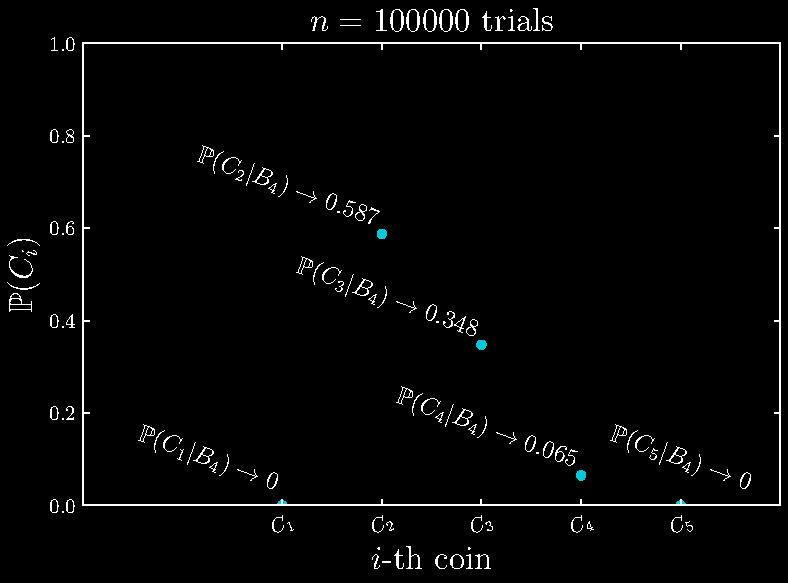
\includegraphics[width=1.0\textwidth]{chap1/chap1ex20c}
\end{center}

% QUESTION 21
\qs{1.10.21}{\textsf{(Computer Experiment.)} Suppose a coin has probability \(p\) of falling heads up. If we flip the coin many times, we would expect the proportion of heads to be near \(p\). We will make this formal later. Take \(p = .3\) and \(n = 1,000\) and simulate \(n\) coin flips. Plot the proportion of heads as a function of \(n\). Repeat for \(p = .03\).}

As intuitively anticipated, for large \(n\), the probability of heads tends towards \(0.3\) or \(0.03\).

\begin{python}
def cointoss():
    coinface = ['H', 'T']
    randomFace = choice(  
    	coinface, 1, p=[0.3, 0.7])
    return randomFace.tolist()[0]

def iteration(n):
    prob = []
    for i in range(1,n+1):
        prob.append(cointoss())
    return prob

def trials(n):
    prob = []
    for i in range(1,n+1):
        prob.append(iteration(i).count('H')/i)
    return prob

n = 1000
\end{python}

\begin{center}
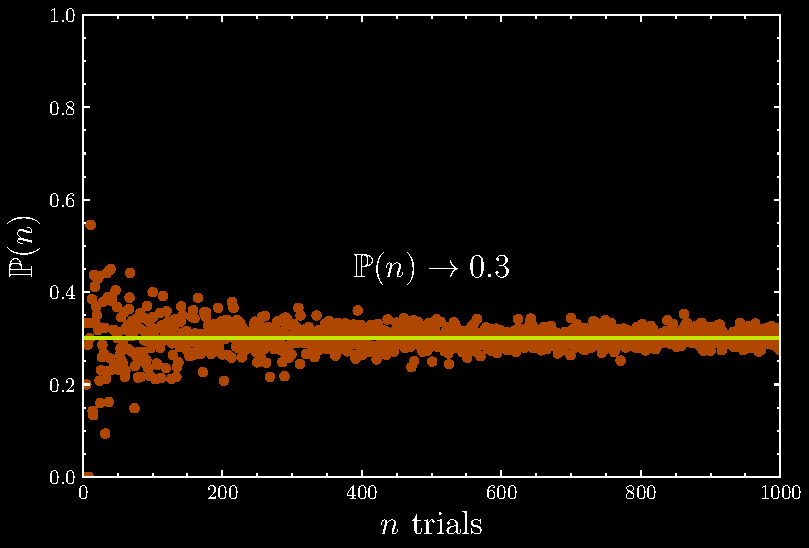
\includegraphics[width=1.0\textwidth]{chap1/chap1ex21i.eps}
\end{center}

\begin{python}
def cointoss():
    coinface = ['H', 'T']
    randomFace = choice(  
        coinface, 1, p=[0.03, 0.97])
    return randomFace.tolist()[0]

def iteration(n):
    prob = []
    for i in range(1,n+1):
        prob.append(cointoss())
    return prob

def trials(n):
    prob = []
    for i in range(1,n+1):
        prob.append(iteration(i).count('H')/i)
    return prob

n = 1000	
\end{python}

\begin{center}
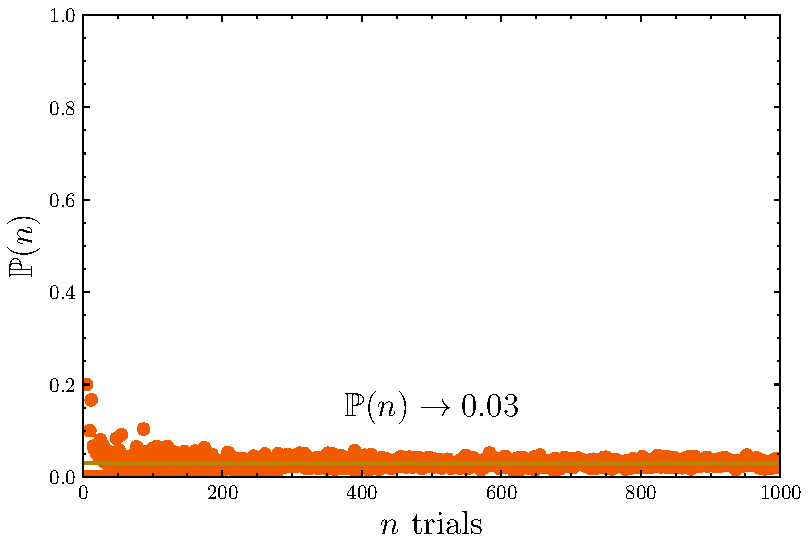
\includegraphics[width=1.0\textwidth]{chap1/chap1ex21ii.eps}
\end{center}

% QUESTION 22
\qs{1.10.22}{\textsf{(Computer Experiment.)} Suppose we flip a coin \(n\) times and let \(p\) denote the probability of heads. Let \(X\) be the number of heads. We call \(X\) a binomial random variable, which is discussed in the next chapter. Intuition suggests that \(X\) will be close to \(np\). To see if this is true, we can repeat this experiment many times and average the \(X\) values. Carry out a simulation and compare the average of the \(X\)'s to \(np\). Try this for \(p = .3\) and \(n = 10, n = 100\), and \(n = 1,000\).}

We run 1,000 trials for 10, 100, and 1,000 flips. The average number of heads for each number of flips are 2.996, 29.958, and 299.92, compared to \(np =\) 3, 30, and 300.

\begin{python}
from statistics import mean

def cointoss():
    coinface = ['H', 'T']
    randomFace = choice(  
        coinface, 1, p=[0.3, 0.7])
    return randomFace.tolist()[0]  

def trials(n, k):
    trials = []
    for j in range(1,k+1):
        probs = []
        for i in range(1,n+1):
            probs.append(cointoss())
        trialcount = probs.count('H')
        trials.append(trialcount)
    return trials

p, n1, n2, n3, k = 0.3, 10, 100, 1000, 1000 
print("Running an experiment of", n1, "flips over", k, 
	"trials, we average", mean(trials(n1,k)), 
	"heads, compared to np =", n1*p)
print("Running an experiment of", n2, "flips over", k, 
	"trials, we average", mean(trials(n2,k)), 
	"heads, compared to np =", n2*p)
print("Running an experiment of", n3, "flips over", k, 
	"trials, we average", mean(trials(n3,k)), 
	"heads, compared to np =", n3*p)
\end{python}

% QUESTION 23
\qs{1.10.23}{\textsf{(Computer Experiment.)} Here we will get some experience simulating conditional probabilities. Consider tossing a fair die. Let \(A = \{2,4,6 \}\) and \(B = \{1,2,3,4 \} \). Then, \(\Prob(A) = 1/2, \Prob(B) = 2/3\) and \(\Prob(AB) = 1/3\). Since \(\Prob(AB) = \Prob(A)\Prob(B)\), the events \(A\) and \(B\) are independent. Simulate draws from the sample space and verify that \(\widehat{\Prob}(AB) = \widehat{\Prob}(A)\widehat{\Prob}(B)\) where \(\widehat{\Prob}(A)\) is the proportion of times \(A\) occurred in the simulation and similarly for \(\widehat{\Prob}(AB)\) and \(\widehat{\Prob}(B)\). Now find two events \(A\) and \(B\) that are not independent. Compute \(\widehat{\Prob}(A), \widehat{\Prob}(B)\) and \(\widehat{\Prob}(AB)\). Compare the calculated values to their theoretical values. Report your results and interpret. }

\begin{python}
def dice():
    return random.randint(1,6)

def rolls(n): 
    sample = []
    for i in range(1,n+1):
        sample.append(dice())
    return sample

n = 10000

# P(A)
prob_A = (rolls(n).count(2) + rolls(n).count(4) + rolls(n).count(6))/n

# P(B)
prob_B = (rolls(n).count(1) + rolls(n).count(2) + rolls(n).count(3) 
         + rolls(n).count(4))/n

# P(AB)
prob_AB = (rolls(n).count(2) + rolls(n).count(4))/n

print("P(A)P(B) =", prob_A*prob_B, "and P(AB) =", prob_AB, 
	". Thus A and B are independent.")
\end{python}

Now suppose we have $A = B = \{k\}$ where $k$ is any integer $1, \dots, 6$. Then $\mathbb{P}(A) = \mathbb{P}(B) = \mathbb{P}(AB) = 1/6$, but $\mathbb{P}(A)\mathbb{P}(B) = 1/36$. Thus $A$ and $B$ are not independent. In general, we can conclude that any event cannot be independent of itself unless the probability of the event is either 0 or 1.

\begin{python}
def dice():
    return random.randint(1,6)

def rolls(n): 
    sample = []
    for i in range(1,n+1):
        sample.append(dice())
    return sample

n = 10000

# P(A)
prob_A = rolls(n).count(1)/n

# P(B)
prob_B = rolls(n).count(1)/n

# P(AB)
prob_AB = rolls(n).count(1)/n

print("P(A)P(B) =", prob_A*prob_B, "and P(AB) =", prob_AB, 
	". Thus A and B are not independent.")
\end{python}

\section{Chapter 2: Random Variables}

\subsection*{Import Packages}

Please see the associated GitHub repo for all code and comments to simulations. [LINK HERE]

\begin{python}
import numpy as np
from numpy.random import choice
import random
import matplotlib.pyplot as plt
import scienceplots
\end{python}

% QUESTION 1
\qs{2.14.1}{Show that
\[
	\Prob(X = x) = F(x^{+}) - F(x^{-}).
\]}
\begin{proof}[Proof] 
	By Lemma 2.15(1), \(\Prob(X = x) = F(x) - F(x^{-})\) where \(F(x^{-}) = \lim_{y \uparrow x} F(y)\). By Theorem 2.8(iii), F is right-continuous, or \(F(x) = F(x^{+})\), where \(F(x^{+}) = \lim_{\substack{ y \rightarrow x \\ y > x}} F(y) \). Thus \(\Prob(X = x) = F(x^{+}) - F(x^{-})\).
\end{proof}

% QUESTION 2
\qs{2.14.2}{Let \(X\) be such that \(\Prob(X = 2) = \Prob(X = 3) = 1/10\) and \(\Prob(X = 5) = 8/10\). Plot the \textsf{CDF} \(F\). Use \(F\) to find \(\Prob(2 < X \le 4.8)\) and \(\Prob(2 \le X \le 4.8)\).}

The \textsf{CDF} is given by

\begin{center}
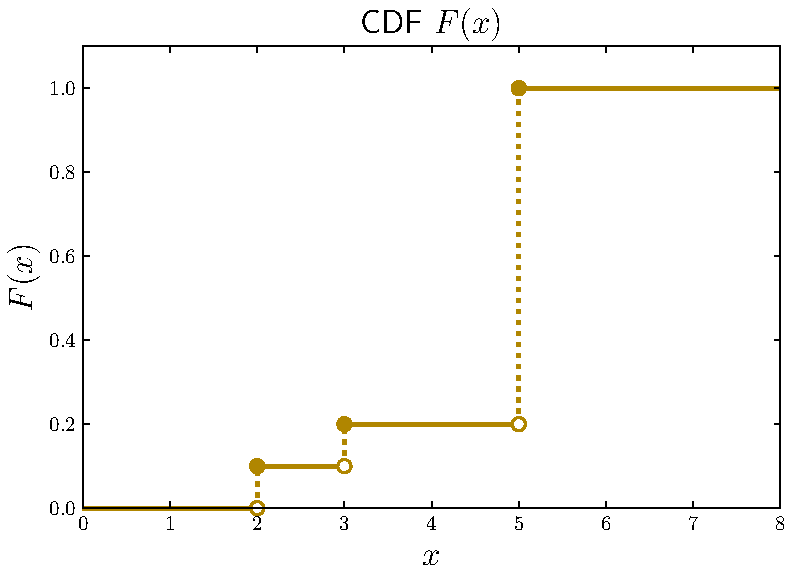
\includegraphics[width=1.0\textwidth]{chap2/chap2ex2.eps}
\end{center}

And the respective probabilities are
\begin{align*}
	\Prob(2 < X \le 4.8) & = \Prob(X \le 4.8) - \Prob(X \le 2) \\
	 & = 2/10 - 1/10 \\
	 & = \boxed{1/10} \\
	\Prob(2 \le X \le 4.8) & = \Prob(X \le 4.8) - \Prob(X < 2) \\
	 & = 2/10 - 0 \\
	 & = \boxed{1/5}
\end{align*}

% QUESTION 3
\qs{2.14.3}{Prove Lemma 2.15.}
\lemma{(Wasserman 2.15)}{Let \(F\) be the \textsf{CDF} for a random variable \(X\). Then:
\begin{enumerate}[label*=\arabic*.]
	\item \(\Prob(X = x) = F(x) - F(x^{-})\) where \(F(x^{-}) = \lim_{y \uparrow x} F(y)\); 
	\item \(\Prob(x < X \le y) = F(y) - F(x)\);
	\item \(\Prob(X > x) = 1 - F(x)\) ;
	\item If \(X\) is continuous then
		\begin{align*}
			F(b) - F(a) & = \Prob(a < X < b) = \Prob(a \le X < b) \\
			 & = \Prob(a < X \le b) = \Prob(a \le X \le b). \\
		\end{align*}
\end{enumerate}}
\begin{proof}[Proof]
	1. Let \(F(x^{-}) = \lim_{y \uparrow x } F(y) \). Then let \(y_{1}, y_{2}, \dots\) be a sequence such that \(y_{1} < y_{2} < \cdots\) and \(\lim_{i} y_{i} = x \). Then let \(A_{i} = (-\infty, y_{i}]\) and \(A = (-\infty, x]\), so \(A = \bigcup_{i=1}^{\infty} A_{i}\) and \(A_{1} \subset A_{2} \subset \cdots \). Thus by continuity of probability, \(\lim_{i} \Prob(A_{i}) = \Prob(\bigcup_{i} A_{i}) = \Prob(A) = F(x) \). But \(\lim_{i} \Prob(A_{i}) = F(x^{-})\) by definition, so we have \(F(x) = F(x^{-})\), implying \(\Prob(X = x) = F(x) - F(x^{-}) = 0\).
	\vspace{12pt}
	\par 2. We have \(\Prob(X \le y) = F(y)\) and \(\Prob(X \le x) = F(x)\). Using mutual exclusivity of the events \(\{\, X \colon X \le x\,\} \text{ and } \{\, X \colon x < X \le y \,\}, \) we can conclude that \(\Prob(X \le x) + \Prob(x < X \le y) = \Prob(X \le y)\) implies \(\Prob(x < X \le y) = F(y) - F(x)\).
\vspace{12pt}
	\par 3. By mutual exclusivity of the events \(\{\,X \colon X > x \,\} \text{ and } \Prob(X \le x)\), we must have \(\Prob(X \le x) + \Prob(X > x) = 1 \), which implies \(\Prob(X > x) = 1 - \Prob(X \le x) = 1 - F(x)\).
\vspace{12pt}
\par 4. Assume \(X\) is continuous. Then \(\Prob(X = a) = \Prob(X = b) = 0\). Since the events \(\{X = a\}, \{\, X \colon a < X < b \,\}, \{X = b \}\) are all disjoint, the desired equalities can be derived from summing the probabilities of the corresponding mutually exclusive events.
\end{proof}

\newpage
% QUESTION 4
\qs{2.14.4}{Let \(X\) have the probability density function
\[
	f_X(x) = \begin{cases}
		1/4  & 0 < x < 1 \\
		3/8  & 3 < x < 5 \\
		0    & \text{otherwise.}
	\end{cases}
\]
\begin{enumerate}[label=(\alph*)]
	\item Find the cumulative distribution function of \(X\).
	\item Let \(Y = 1/X\). Find the probability density function \(f_Y(y)\) for \(Y\). Hint: Consider three cases \(\frac{1}{5} \le y \le \frac{1}{3}, \frac{1}{3} \le y \le 1, \text{ and } y \ge 1.\)
\end{enumerate}
}
(a) To find the \textsf{CDF}, we find how the area under the \textsf{PDF} changes as \(x\) increases. The direct approach is to integrate each segment of the piecewise \textsf{PDF}, with some nuance -- as \(x\) moves between 1 and 3, since the \textsf{PDF} is zero here, there is no contribution to the \textsf{CDF}, and so \(F(x)\) stays at \(1/4\) on this segment. Additionally, once we reach the \((3,5)\) segment, we not only integrate \(3/8\) over the aforementioned interval, but add \(1/4\) to reflect the \textit{cumulative} probability. Proceeding in this manner, the \textsf{CDF} is
\[
	F_X(x) = \begin{cases}
		0 & x \le 0 \\
		x/4 & 0 < x < 1 \\
		1/4 & 1 \le x \le 3 \\
		1/4 + 3(x-3)/8 & 3 < x < 5 \\
		1 & 5 \le x	
	\end{cases} 
\]
Graphing the \textsf{PDF} and \textsf{CDF}:

\begin{center}
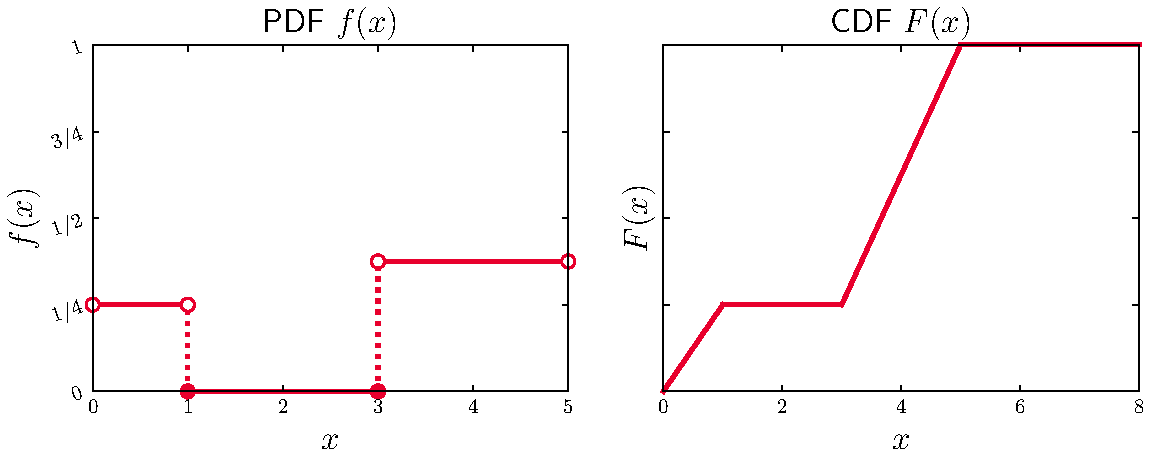
\includegraphics[width=1.0\textwidth]{chap2/chap2ex4a.eps}
\end{center}
\vspace{12pt}
	\par (b) To derive \(F_Y(y)\), we begin with
	\begin{align*}
		F_Y(y) & = \Prob(Y \le y) \\
		 & = \Prob(1/X \le y) \\
		 & = \Prob(1/y \le X) \\
		 & = 1 - \Prob(X < 1/y)
	\end{align*}

Since \(f_X(x)\) is given as a piecewise function, we must calculate the segments of the \textsf{CDF} \(F_Y(y)\), and consequently the \textsf{PDF} \(f_Y(y)\), separately.

Note also that
\[
	\frac{d}{dy} F_Y(y) = f_Y(y)
\]

\underline{Case 1:} \(1/5 < y < 1/3\) corresponding to \(3 < x < 5\)
\begin{align*}
	F_Y(y) & = 1 - \Prob(X < 1/y) \\
	 & = 1 - \left(\frac{1}{4} + \frac{3(1/y - 3)}{8} \right)   \\
	 & = \frac{15}{8} - \frac{3}{8y} \\
	\implies f_Y(y) & = \boxed{\frac{3}{8y^{2}}}
\end{align*}

\underline{Case 2:} \(1/3 \le y \le 1\) corresponding to \(1 \le x \le 3\)
\begin{align*}
	F_Y(y) & = 1 - \Prob(X < 1/y) \\
	 & = 1 - 1/4 \\
	 & = 3/4 \\
	\implies f_Y(y) & = \boxed{0}
\end{align*}

Intuitively, since \(f_X(x) = 0\) here, \(f_Y(y) = \boxed{0}\).

\underline{Case 3:} \(y > 1\) corresponding to \(0 < x < 1\)
\begin{align*}
	F_Y(y) & = 1 - \Prob(X < 1/y) \\
	 & = 1 - \frac{1}{4y} \\
	\implies f_Y(y) & = \boxed{\frac{1}{4y^{2}}}
\end{align*}
Thus the \textsf{CDF} and \textsf{PDF} of \(Y\) is given by
\[\begin{aligned}
	F_Y(y) & = \begin{cases}
		0 & y \le 1/5 \\
		15/8 - 3/8y & 1/5 < y < 1/3 \\
		3/4 & 1/3 \le y \le 1 \\
		1 - 1/4y & y > 1 
	\end{cases} \\
	f_Y(y) & = \begin{cases}
		3/8y^{2} & 1/5 < y < 1/3 \\
		1/4y^{2} & y > 1 \\
		0 & \text{otherwise}	
	\end{cases}
 \end{aligned}
\]
Graphing the \textsf{PDF} and \textsf{CDF}:
\begin{center}
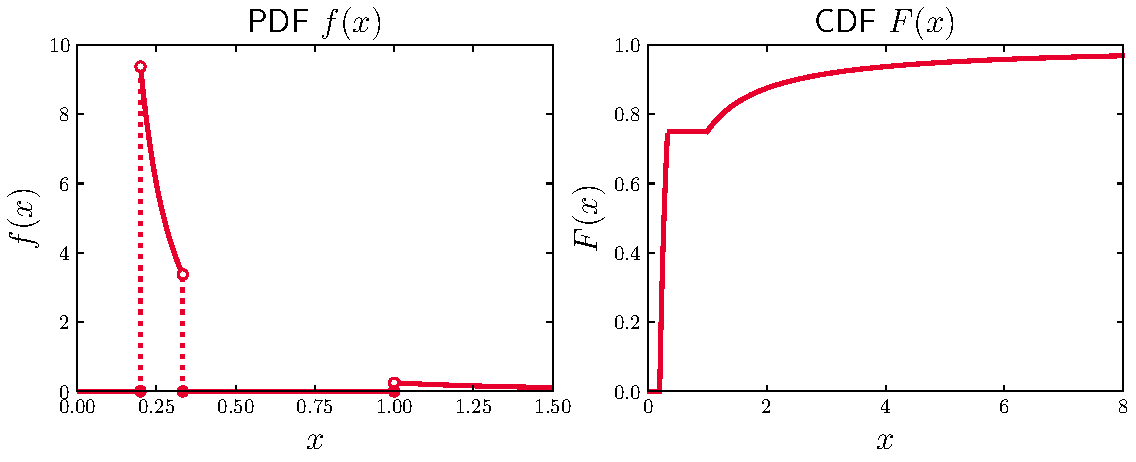
\includegraphics[width=1.0\textwidth]{chap2/chap2ex4b.eps}
\end{center}

% QUESTION 5
\qs{2.14.5}{Let \(X\) and \(Y\) be discrete random variables. Show that \(X\) and \(Y\) are independent if and only if \(f_{X,Y}(x,y) = f_{X}(x)f_{Y}(y)\) for all \(x\) and \(y\).}
\begin{proof}[Proof] 
\((\implies)\) Let \(X \sqcup Y\). Then for all \(x, y\), \(\Prob(X = x, Y=y) = \Prob(X = x)\Prob(Y = y)\). Since \(f_X(x) = \Prob(X = x), f_Y(y) = \Prob(Y = y)\), and \(f_{X,Y}(x,y) = \Prob(X = x, Y = y)\), we have
\[
	f_{X,Y}(x,y) = f_{X}(x)f_{Y}(y)
\]
\par \( (\impliedby) \) Let \(f_{X,Y}(x,y) = f_{X}(x)f_{Y}(y)\) for all \(x, y\). Since \(f_{X,Y}(x,y) = \Prob(X=x, Y=y)\), \(f_{X}(x) = \Prob(X=x)\) and \(f_{Y}(y) = \Prob(Y=y)\), we must have
\[
	\Prob(X=x, Y=y) = \Prob(X=x)\Prob(Y=y)
\]
for all \(x,y\). Thus \(X \sqcup Y\).
\end{proof}

% QUESTION 6
\qs{2.14.6}{Let \(X\) have distribution \(F\) and density function \(f\) and let \(A\) be a subset of the real line. Let \(I_{A}(x)\) be the indicator function for \(A\):
\[
	I_{A}(x) = \begin{cases}
		1 & x \in  A \\
		0 & x \not\in A. \\
	\end{cases}
\]
Let \(Y = I_{A}(X)\). Find an expression for the cumulative distribution of \(Y\). (Hint: first find the probability mass function for \(Y\).)}
Let \(Y = I_{A}(x)\). Then
\[
	f_{Y}(y) = \begin{cases}
		\Prob(Y = 1) = \int_{A} f \ dx & x \in A \\
		\Prob(Y = 0) = 1 - \int_{A} f \ dx & x \not\in A \\
		0 & \text{otherwise}
	\end{cases}
\]
which implies
\[
	F_{Y}(y) = \begin{cases}
		0 & y < 0 \\
		1 - \int_{A} f \ dx  & 0 \le y < 1 \\
		1 & y \ge 1 \\
	\end{cases}
\]
% QUESTION 7
\qs{2.14.7}{Let \(X\) and \(Y\) be independent and suppose that each has a \(\Uniform(0,1)\) distribution. Let \(Z = \min\{X,Y\}\). Find the density \(f_{Z}(z)\) for \(Z\). Hint: It might be easier to first find \(\Prob(Z > z)\).}

One can follow the hint and observe that \(\Prob(Z > z)\) if and only if 
\[
	\Prob(X > z)\Prob(Y > z) = (1 - \Prob(X < z))(1 - \Prob(Y < z)) = (1 - F_{X}(z))(1 - F_{Y}(z))
\]
and applying the fact that \(F_{X}(x), F_{Y}(y)\) both follow a standard uniform distribution. We will also attempt to derive the density \(f_{Z}(z)\) by modeling the mutual exclusivity of either \(X\) or \(Y\) being the minimum.

We define \(Z\) as
\[
	Z = \min\{X,Y\} = \begin{cases}
		X & x < y \\
		Y & y < x \\
	\end{cases} 
\]
Since \(X,Y\) have standard uniform distribution, it must also be the case that \(0 < z < 1\) has non-zero probability, and zero probability otherwise.

Our task is to derive \(\Prob(0 < Z < z)\). Either \(X \le Y\) or \(Y \le X\), and in those cases, we must also have \(X \le z\) and \(Y \le z\), respectively. Thus we derive \(F_{Z}(z)\) on this interval:
\begin{align*}
	\Prob(0 < Z \le z) & = \Prob(X \le z)\Prob(X \le Y) + \Prob(Y \le z)\Prob(Y \le X) \\
	 & = \int^{z}_{0} \int^{1}_{x}  \ dy  \ dx + \int^{z}_{0} \int^{1}_{y}  \ dx  \ dy  \\
	 & = \boxed{2z - z^{2}}
\end{align*}
Similarly, we look at \(\Prob(z < Z < 1)\), which corresponds to \(1 - F_{Z}(z)\). As in the previous case, either \(X \le Y\) or \(Y \le X\), but this time these cases correspond to \(X > z\) and \(Y > z\). We derive
\begin{align*}
	\Prob(z < Z < 1) & = \Prob(X > z)\Prob(X \le Y) + \Prob(Y > z)\Prob(Y \le X) \\
	 & = \int^{1}_{z} \int^{1}_{x}  \ dy  \ dx + \int^{1}_{z} \int^{1}_{y}  \ dx  \ dy  \\
	 & = \boxed{1 - 2z + z^{2}}
\end{align*}
Either way, we can conclude
\begin{align*}
	F_{Z}(z) & = \begin{cases}
		0 & z \le 0 \\
		2z - z^{2} & 0 < z < 1 \\
	        1 & z \ge 1
	\end{cases} \\
	f_{Z}(z) & = \begin{cases}
		2(1-z) & 0 < z < 1  \\
		0 & \text{otherwise} \\
	\end{cases} \\
\end{align*}
And as anticipated, our theoretical work aligns with the empirical:
\begin{center}
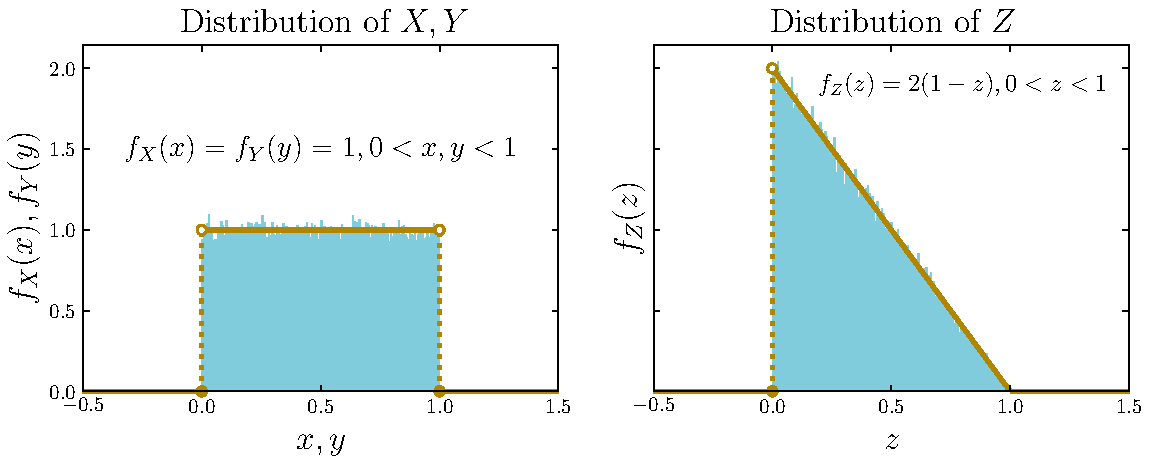
\includegraphics[width=1.0\textwidth]{chap2/chap2ex7.eps}
\end{center}

% QUESTION 8
\qs{2.14.8}{Let \(X\) have \textsf{CDF} \(F\). Find the \textsf{CDF} of \(X^{+} = \max\{0,X\}\).}
Observe that \(\Prob(X^{+} = 0) = \Prob(X \le 0) = F(0)\). For \(X > 0\), we have \(\Prob(X^{+} = X) = \Prob(0 < X \le x) = F(x) - F(0)\). Then the \textsf{CDF} of \(X^{+}\) is
\[
	F_{X^{+}}(X^{+}) = \begin{cases}
		F_{X}(0) & X \le 0, X^{+} = 0 \\
		F_{X}(x) & X > 0, X^{+} = X > 0 \\
	\end{cases}
\]

% QUESTION 9
\qs{2.14.9}{Let \(X \sim \Exp(\beta)\). Find \(F(x)\) and \(F^{-1}(q)\).}
\[
	F(x) = \int^{x}_{0} \frac{1}{\beta}\exp(-x/\beta) \ dx = 1 - \exp(-x/\beta),\quad x > 0 \\
\]
Let \(q = F(x)\). Then \(q = 1 - \exp(-x/\beta )\) implies
\begin{align*}
	\implies & \exp(-x/\beta ) = 1-q \\
	\implies & \boxed{x = -\beta \ln(1-q)}, \quad 0 \le q < 1
\end{align*}

% QUESTION 10
\qs{2.14.10}{Let \(X\) and \(Y\) be independent. Show that \(g(X)\) is independent of \(h(Y)\) where \(g\) and \(h\) are functions.}
\begin{proof}[Proof] 
Let \(X \sqcup Y\). Consider the joint probability \(\Prob(X,Y)\). By premise, \(\Prob(X,Y) = \Prob(X)\Prob(Y)\) for all \(x,y\). Now consider \(g(X), h(Y)\). Let 
\begin{align*}
	A & = \{\, X \colon g(X) \in A' \,\} \\
	B & = \{\, Y \colon h(Y) \in B'\,\}
\end{align*}
where \(A', B'\) are the sets containing the respective transformations of \(X \in A, Y \in B\). The intuition to have here is that the "link" between \(X \in A\) and \(g(X) \in A'\) preserves the independence of the former in the latter under transformation.

Then we have
\begin{align*}
	\Prob(g(X) \in A') & = \Prob(X \in A) \\
	\Prob(h(Y) \in B') & = \Prob(Y \in B) \\
	\implies \Prob(g(X) \in A', h(Y) \in B') & = \Prob(X \in A, Y \in B)
\end{align*}
Applying independence on the last equality,
\[
	\Prob(g(X \in A'), h(y \in B')) = \Prob(g(X \in A'))\Prob(h(Y \in B'))	
\]
ascertaining that \(g(X) \sqcup h(X)\).
\end{proof}

% QUESTION 11
\qs{2.14.11}{Suppose we toss a coin once and let \(p\) be the probability of heads. Let \(X\) denote the number of heads and let \(Y\) denote the number of tails.
\begin{enumerate}[label=(\alph*)]
	\item Prove that \(X\) and \(Y\) are dependent.
	\item Let \(N \sim \Poisson(\lambda)\) and suppose we toss a coin \(N\) times. Let \(X\) and \(Y\) be the number of heads and tails. Show that \(X\) and \(Y\) are independent.
\end{enumerate}}
\begin{proof}[Proof] 
(a) We have \(\Prob(X=1) = p\) and \(\Prob(Y=1) = 1-p\), where \(X,Y\) are the number of heads and tails. Note that \(\Prob(X=1,Y=1) = 0\), as we can only have one head or one tail after a single toss. But clearly \(\Prob(X=1)\Prob(Y=1) = p(1-p) = 0\) for non-zero \(p\), so \(X, Y\) are dependent.
\vspace{12pt}
\par (b) The intuition is to decompose the joint probability \(f_{X,Y}(x,y)\) into \(g(x)h(y)\), where \(g(x), h(y)\) are \textit{any} functions (not necessarily densities). We can equivalently find the joint probability that we toss \(X = x\) heads \textit{and} toss the coin \(N\) times:
\begin{align*}
	\Prob(X = x, Y = y) & = \Prob(X = x, N = x+y) \\
			    & = \binom{N}{x} p^{x}(1-p)^{N-x}e^{-\lambda} \frac{\lambda^{N}}{N!} \\
			    & = \binom{x+y}{x} p^{x}(1-p)^{y} e^{-\lambda} \frac{\lambda^{x+y}}{(x+y)!} \\
			    & = \frac{(x+y)!}{x!y!} p^{x}(1-p)^{y}e^{-\lambda} \frac{\lambda^{x+y}}{(x+y)!} \\
			    & = \underbrace{\left(e^{-\lambda} \frac{\lambda^{x}}{x!}p^{x}  \right)}_{g(x)} \underbrace{\left( \frac{\lambda^{y}}{y!} (1-p)^{y} \right) }_{h(y)} 
\end{align*}
\end{proof}

\newpage
% QUESTION 12
\qs{2.14.12}{Prove Theorem 2.33.}
\thm{(Wasserman 2.33)}{Suppose that the range of \(X\) and \(Y\) is a (possibly infinite) rectangle. If \(f(x,y) = g(x)h(y)\) for some functions \(g\) and \(h\) (not necessarily probability density functions) then \(X\) and \(Y\) are independent.}
\begin{proof}[Proof] 
Let \(X, Y\) have density \(f(x,y)\), and define
\[
	A = \{\,(x,y) \colon x > 0, y > 0 \,\}
\]
Then
\begin{align*}
	1 & = \int \int_{A} f(x,y)  \ dx  \ dy  \\
	  & = \underbrace{\int^{\infty}_{0} g(x) \ dx}_{c} \underbrace{\int^{\infty}_{0} h(y) \ dy }_{1/c}
\end{align*}
where \(0 < c < 1\). Let \(f_{X}(x) = \frac{1}{c} g(x), x > 0\) and \(f_{Y}(y) = ch(y), y > 0\). Then
\[
	f(x,y) = g(x)h(x) = \left( \frac{1}{c} g(x) \right) \left( c h(y) \right) = f_{X}(x) f_{Y}(y)
\]
for all \(x, y\). Thus \(X \sqcup Y\).
\end{proof}

% QUESTION 13
\qs{2.14.13}{Let \(X \sim N(0,1\) and let \(Y = e^{X}\).
\begin{enumerate}[label=(\alph*)]
	\item Find the \textsf{PDF} for \(Y\). Plot it.
	\item \textsf{(Computer Experiment.)} Generate a vector \(x = (x_{1},\dots, x_{10,000})\) consisting of \(10,000\) random standard Normals. Let \(y = (y_{1},\dots, y_{10,000})\) where \(y_{i} = e^{x_{i}}\). Draw a histogram of \(y\) and compare it to the \textsf{PDF} you found in part (a).
\end{enumerate}}
\begin{align*}
	F_{Y}(y) & = \Prob(Y \le y) \\
	 & = \Prob(e^{X} \le y) \\
	 & = \Prob(X \le \ln y) \\
	 & = \frac{1}{\sqrt{2\pi}} \int^{\ln y}_{-\infty} \exp \left( -\frac{x^{2}}{2} \right)  \ dx \\
	 & = \frac{1}{\sqrt{2\pi}} \int^{0}_{-\infty} \exp \left( -\frac{x^{2}}{2} \right)  \ dx + \frac{1}{2\pi} \int^{\ln y}_{0} \exp \left( -\frac{x^{2}}{2} \right)  \ dx  
\end{align*}
Applying the Leibniz rule, we find
\[
	F_{Y}'(y) = f_{Y}(y) = \frac{1}{y\sqrt{2 \pi}}  \exp \left( -\frac{1}{2} (\ln y)^{2} \right), \quad y > 0
\]
\vspace{12pt}
\par (b) Our theoretical and empirical results agree:
\begin{center}
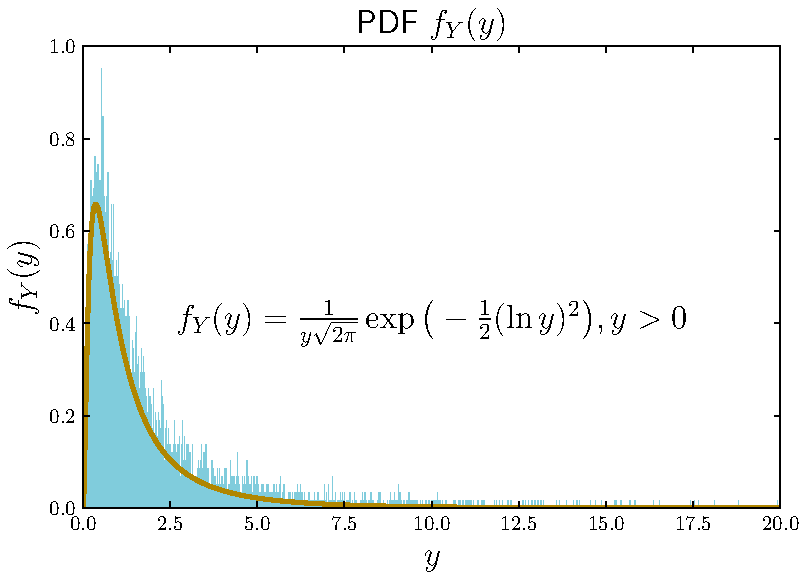
\includegraphics[width=1.0\textwidth]{chap2/chap2ex13.eps}
\end{center}

% QUESTION 14
\qs{2.14.14}{Let \((X,Y)\) be uniformly distributed on the unit disk \(\{\,(x,y) \colon x^{2} + y^{2} \le 1 \,\}\). Let \(R = \sqrt{X^{2}+Y^{2}}\). Find the \textsf{CDF} and \textsf{PDF} of \(R\).}

For a joint density involving uniformly distributed variables, \(f(x,y) = 1/\text{area}(A)\), where \(A\) is the region over which the densities of the constituent variables are defined and non-zero. Since we choose uniformly distributed \((x,y)\) over the unit circle, its area is \(A = \pi \).

Integrating in polar coordinates, we derive for \(0 < r < 1\):
\[
	F_{R}(r) = \int^{2 \pi }_{0} \int^{r}_{0} \frac{1}{\pi }s \ ds   \ d \theta = \int^{2 \pi }_{0} \frac{1}{\pi }\frac{r^{2}}{2} \ d\theta = r^{2} 
\]
giving us the \textsf{CDF} and \textsf{PDF}:
\begin{align*}
	F_{R}(r) & = \begin{cases}
		0 & r \le 0 \\
		r^{2} & 0 < r <  \\
	        1 & r \ge 1
	\end{cases} \\
	F'_{R}(r) = f_{R}(r) & = 2r, \quad 0 < r < 1 \\
\end{align*}

Empirically generating the \((x,y)\)'s agrees with the theoretically derived density:
\begin{center}
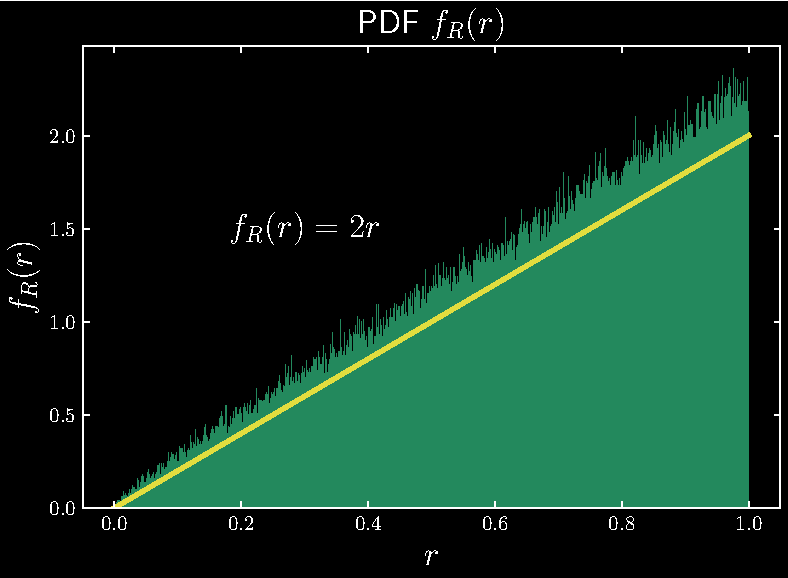
\includegraphics[width=1.0\textwidth]{chap2/chap2ex14.eps}
\end{center}

% QUESTION 15
\qs{2.14.15}{\textsf{(A universal random number generator.)} Let \(X\) have a continuous, strictly increasing \textsf{CDF} \(F\). Let \(Y = F(X)\). Find the density of \(Y\). This is called the probability integral transform. Now let \(U \sim \Uniform(0,1)\) and let \(X = F^{-1}(U)\). Show that \(X \sim F\). Now write a program that takes \(\Uniform(0,1)\) random variables and generates random variables from an \(\Exp(\beta )\) distribution.}
\begin{proof}[Proof] 
By assumption, \(F_{X}(x)\) is strictly increasing and continuous. This means \(F_{X}(x)\) is a bijection, and has an inverse \(F_{X}^{-1}(x)\). We use this fact to derive
\begin{align*}
	F_{Y}(y) & = \Prob(Y \le y) \\
	 & = \Prob(F_{X}(x) \le y) \\
	 & = F_{X}(F_{X}^{-1}(y)) \\
	 & = y \\
	\implies F_{Y}^{-1}(y) = f_{Y}(y) & = 1
\end{align*}

A shocking result! All probability integral transforms of \textit{any} continuous distribution give us the density to the standard uniform distribution. 

For the next result, let \(U \sim \Uniform(0,1)\) and \(X = F^{-1}(U)\). The intuition to have here is that \(F^{-1}\) is a quantile function! Again appealing to the bijectivity of \(F\), we have \(F(X) = U\). Since \(F: X \rightarrow [0,1]\) and invoking the preservation of monotonocity under an inverse operation \((x_{1} < x_{2} \iff F(x_{1}) < F(x_{2}))\), we have 
\[
	\Prob(X \le x) = \Prob(F^{-1}(U) \le x) = \Prob(U \le F(x)) = F(x)
\]
Thus we must have \(X \sim F\).
\end{proof}

The quantile function for the \(\Exp(\beta )\) distribution is \(F^{-1}(q) = -\beta \ln(1-q)\). Generating the exponential distribution via the probability integral transform:

\begin{center}
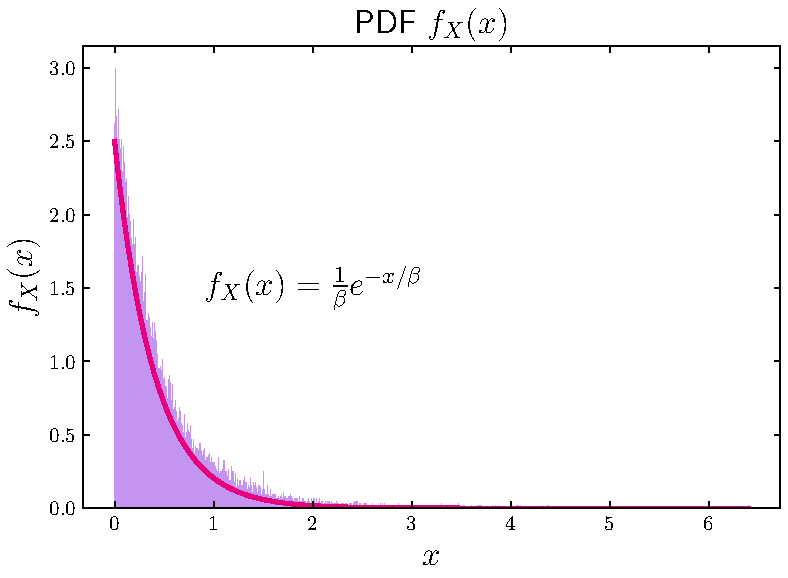
\includegraphics[width=1.0\textwidth]{chap2/chap2ex15.eps}
\end{center}

% QUESTION 16
\qs{2.14.16}{Let \(X \sim \Poisson(\lambda )\) and \(Y \sim \Poisson(\mu)\) and assume that \(X\) and \(Y\) are independent. Show that the distribution of \(X\) given that \(X + Y = n\) is \(\binomial(n,\pi )\) where \(\pi = \lambda / (\lambda + \mu)\).

Hint 1: You may use the following fact: If \(X \sim \Poisson(\lambda )\) and \(Y \sim \Poisson(\mu)\), and \(X\) and \(Y\) are independent, then \(X + Y \sim \Poisson(\mu + \lambda )\).

Hint 2: Note that \(\{X = x, X + Y = n \} = \{X = x, Y = n-x \}\).}
\begin{proof}[Proof] 
By definition of the Poisson distribution:
\begin{align*}
	f(X+Y = n) & = e^{-(\lambda + \mu)} \frac{(\lambda + \mu)^n}{n!} \\
	f(X = x, Y = n-x) & = e^{-\lambda } \frac{\lambda^{x}}{x!} e^{-\mu} \frac{\mu^{n-x}}{(n-x)!}
\end{align*}
Proceeding to set up the conditional probability:
\begin{align*}
	f(X  \mid  X + Y = n) & = \frac{e^{-\lambda } \frac{\lambda^{x}}{x!} e^{-\mu} \frac{\mu^{n-x}}{(n-x)!}}{e^{-(\lambda + \mu)} \frac{(\lambda + \mu)^n}{n!}} \\
			 & = \frac{\lambda^{x} \mu^{n-x}}{(\lambda + \mu)^{n}} \frac{n!}{(n-x)!x!} \\
			 & = \binom{n}{x} \left( \frac{\lambda }{\lambda + \mu} \right)^{x} \left( \frac{\mu}{\lambda + \mu} \right)^{n-x} \\
			 & = \binom{n}{x} \left( \frac{\lambda }{\lambda + \mu} \right)^{x} \left( 1 - \frac{\lambda }{\lambda + \mu} \right)^{n-x}  
\end{align*}
ascertaining that \(X  \mid  X + Y = n \sim \binomial(n,\pi )\) for \(\pi = \lambda / (\lambda + \mu)\).
\end{proof}

% QUESTION 17
\qs{2.14.17}{Let
\[
	f_{X,Y}(x,y) = \begin{cases}
		c(x+y^{2}) & 0 \le x < 1 \text{ and } 0 \le y \le 1 \\
		0 & \text{otherwise.} \\
	\end{cases}
\]
Find \(\Prob(X < \frac{1}{2}  \mid  Y = \frac{1}{2})\).}

First we find the marginal density function of \(y\):
\[
	f_{Y}(y) = \int^{1}_{0} c(x+y^{2}) \ dx = c(1/2 + y^{2})
\]
Then the conditional density function is
\[
	f_{X \mid Y}(x \mid y) = \frac{x + y^{2}}{1/2 + y^{2}}
\]
Now we calculate the desired probability:
\begin{align*}
	\Prob(X < 1/2  \mid  Y = 1/2) & = \int^{1/2}_{0}  f_{X \mid Y}(x  \mid  1/2) \ dx  \\
	 & = \int^{1/2}_{0} \frac{x + 1/4}{1/2 + 1/4} \ dx  \\
	 & = \frac{1/8 + 1/8}{1/2 + 1/4} \\
	 & = \boxed{1/3}
\end{align*}

\newpage
% QUESTION 18
\qs{2.14.18}{Let \(X \sim N(3,16)\). Solve the following using the Normal table and using a computer package.
\begin{enumerate}[label=(\alph*)]
	\item Find \(\Prob(X < 7)\).
	\item Find \(\Prob(X > -2)\).
	\item Find \(x\) such that \(\Prob(X > x) = .05\).
	\item Find \(\Prob(0 \le X < 4)\).
	\item Find \(x\) such that \(\Prob( \mid X \mid  >  \mid x \mid ) = .05\).  
\end{enumerate}}
It is best to use scipy.stats here:
\begin{python}
from scipy.stats import norm

normal_dist = norm(3, 4)

# (a)
prob_a = normal_dist.cdf(7)
print("The probability for (a) is", prob_a)

# (b)
prob_b = 1 - normal_dist.cdf(-2)
print("The probability for (b) is", prob_b)

# (c)
x_c = normal_dist.ppf(0.95)
print("The value of x for (c) is", x_c)

# (d)
prob_d = normal_dist.cdf(4) - normal_dist.cdf(0)
print("The probability for (d) is", prob_d)

# (e)
x = np.arange(9.5,9.7,0.00000001)
array = np.round(normal_dist.cdf(x) - normal_dist.cdf(-x), decimals=9)
index = np.where(array == 0.95)
x_e = x[index[0]]
print("Some values of x for (e) are", x_e)
\end{python}

Using the above calculations:

\begin{enumerate}[label=(\alph*)]
	\item \(\Prob(X < 7) = 0.841\)
	\item \(\Prob(X > -2) = 0/894\)
	\item \(x = 9.579\)
	\item \(\Prob(0 \le X < 4) = 0.372\)
	\item \(x = 9.611\)
\end{enumerate}

For (e), the intuition behind the absolute values is to evaluate the probabilities at the tails of the distribution. Given \( \mid x \mid  > 0\), we can equivalently write
\begin{align*}
	\Prob( \mid X \mid  >  \mid x \mid ) & = \Prob(X >  \mid x \mid ) + \Prob(X < - \mid x \mid ) \\
	 & = 1 - \Prob(X <  \mid x \mid ) + \Prob(X < - \mid x \mid ) = 0.05 \\
	\implies 0.95 & = \Prob(X <  \mid x \mid ) - \Prob(X < - \mid x \mid )
\end{align*}

Numerically iterating enables us to identify the value of \( \mid x \mid  = x\) without needing to convert to a standard normal distribution.

% QUESTION 19
\qs{2.14.19}{Prove formula (2.12).}
\prp{(Wasserman Formula 2.12)}{For a strictly monotone increasing or strictly monotone decreasing function \(r(X)\) with an inverse \(s = r^{-1}\), we have
\[
	f_{Y}(y) = f_{X}(s(y)) \bigg| \frac{d s(y) }{d y}  \bigg| .
\]}
\begin{proof}[Proof] 
\underline{Case 1: Increasing \(r(X).\)} Derive
\begin{align*}
	F_{Y}(y) = \Prob(Y \le y) & = \Prob(r(X) \le y) \\
	 & = \Prob(X \le r^{-1}(y)) \\
	 & = \Prob(X \le s(y)) \\
	 & = \int^{s(y)}_{-\infty} f_{X}(x) \ dx 
\end{align*}
Implying \(F'_{Y}(y) = f_{Y}(y) = f_{X}(s(y)) \frac{d s(y)}{d y} \). Note that since \(r(X)\) is strictly monotone increasing by premise, \(ds(y)/dy > 0\).
\vspace{12pt}
\par \underline{Case 2: Decreasing \(r(X)\).} Derive
\begin{align*}
	F_{Y}(y) = \Prob(Y \le y) & = \Prob(r(X) \le y)  \\
	 & = \Prob(X \ge r^{-1}(y)) \\
	 & = \Prob(X \ge s(y)) \\
	 & = 1 - \Prob(X \le s(y)) \\
	 & = 1 - \int^{s(y)}_{-\infty} f_{X}(x) \ dx \\
	F'_{Y}(y) = f_{Y}(y) & = - f_{X}(s(y)) \frac{d s(y)}{d y} 
\end{align*}
where the second equality follows because \(r(X)\) is strictly monotonically \textit{decreasing}. That same fact also allows us to say that \(ds(y) / dy < 0\). To encapsulate both the increasing and decreasing cases, we have
\[
	f_{Y}(y) = f_{X}(s(y)) \bigg| \frac{d s(y)}{d y}  \bigg| 
\]
\end{proof}

% QUESTION 20
\qs{2.14.20}{Let \(X,Y \sim \Uniform(0,1)\) be independent. Find the \textsf{PDF} for \(X-Y\) and \(X/Y\).}

The joint probability density function is given by
\[
	f_{X,Y}(x,y) = \begin{cases}
		1 & 0 < x, y < 1 \\
		0 & \text{otherwise} \\
	\end{cases}
\]
\underline{\(X - Y\)}

\par Illustrations are particularly useful here to understand where the piecewise segments of \(f_{Z}(z)\) are defined.

Given \(Z = X-Y\), it must be the case that either \(0 < z < 1\) or \(-1 < z < 0\). To find \(A_{z}\), the support for the probability density function, we find all \(x, y\) satisfying
\[
	A_{z} = \{\,(x,y) \colon x - y \le z \,\}
\]
Now, there is a nice geometric intuition in that the piecewise \textsf{CDF} is given by the area of the support on each interval \(0 < z < 1, -1 < z < 0\). Graphically, this support in the first and second cases is:

\begin{center}
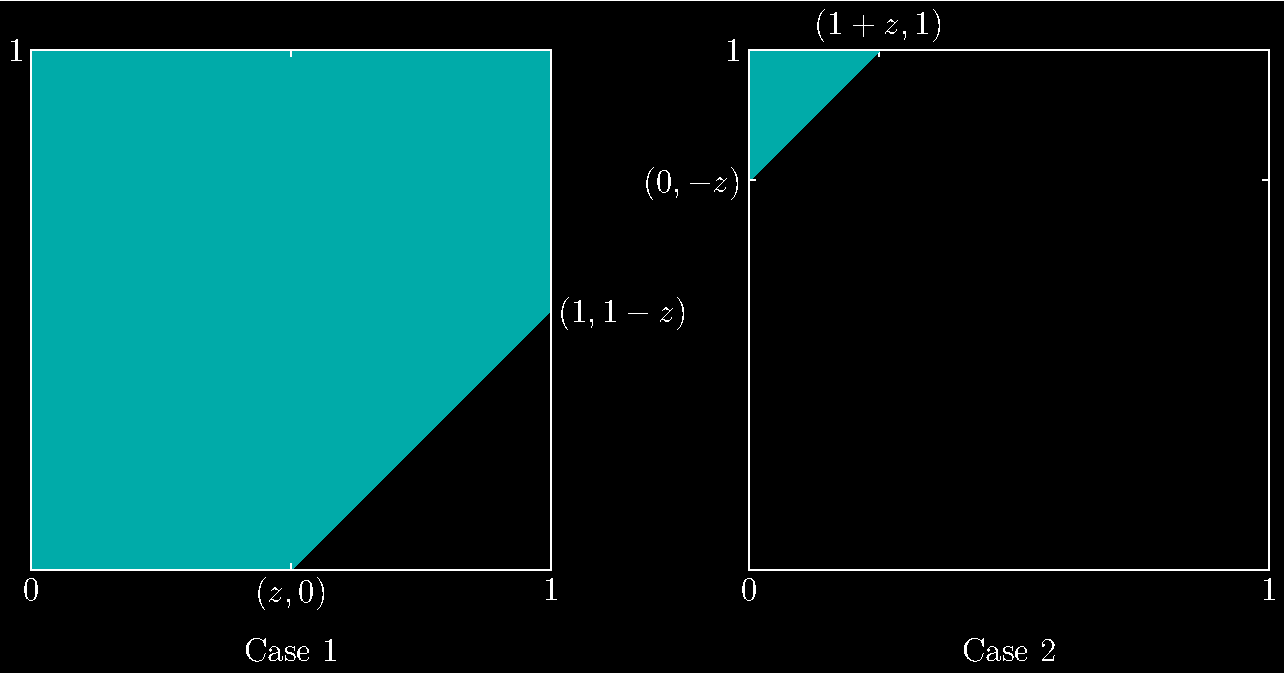
\includegraphics[width=1.0\textwidth]{chap2/chap2ex20i.eps}
\end{center}

Calculating the area of the shaded parts, we can derive the \textsf{CDF} as
\[
	F_{Z}(z) = \begin{cases}
		0 & z < -1 \\
		\frac{1}{2}(1+z)^{2} & -1 < z < 0 \\
		1 - \frac{1}{2}(1-z)^{2} & 0 < z < 1 \\
		1 & z > 1
	\end{cases}
\]
and consequently, the \textsf{PDF} is
\[
	f_{Z}(z) = \begin{cases}
		1 + z & -1 < z < 0 \\
		1 - z & 0 < z < 1 \\
		0 & \text{otherwise}
	\end{cases}
\]

which agrees with our empirical simulation:
\begin{center}
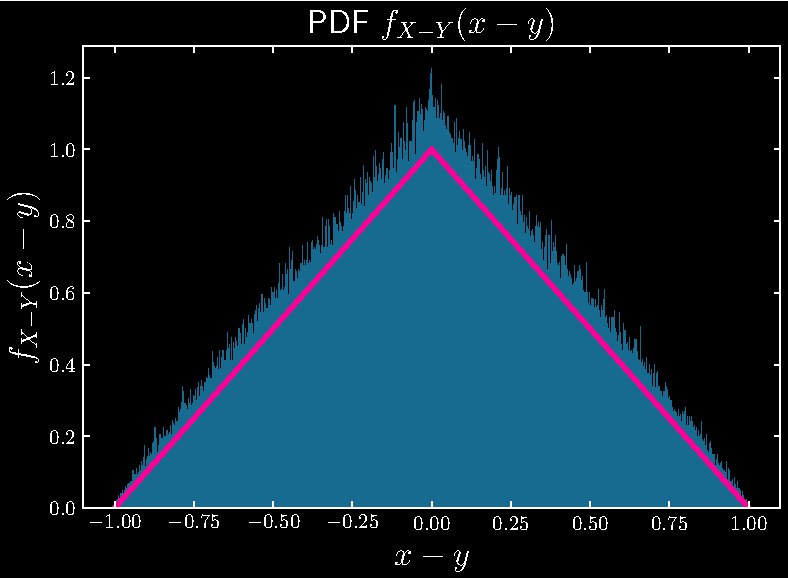
\includegraphics[width=1.0\textwidth]{chap2/chap2ex20iii.eps}
\end{center}

\underline{\(X/Y\)}
\par Once again finding the supports for \(Z = X/Y\), observe that the intervals we examine are \(0 < z < 1\) and \(z > 1\). The areas are graphed as

\begin{center}
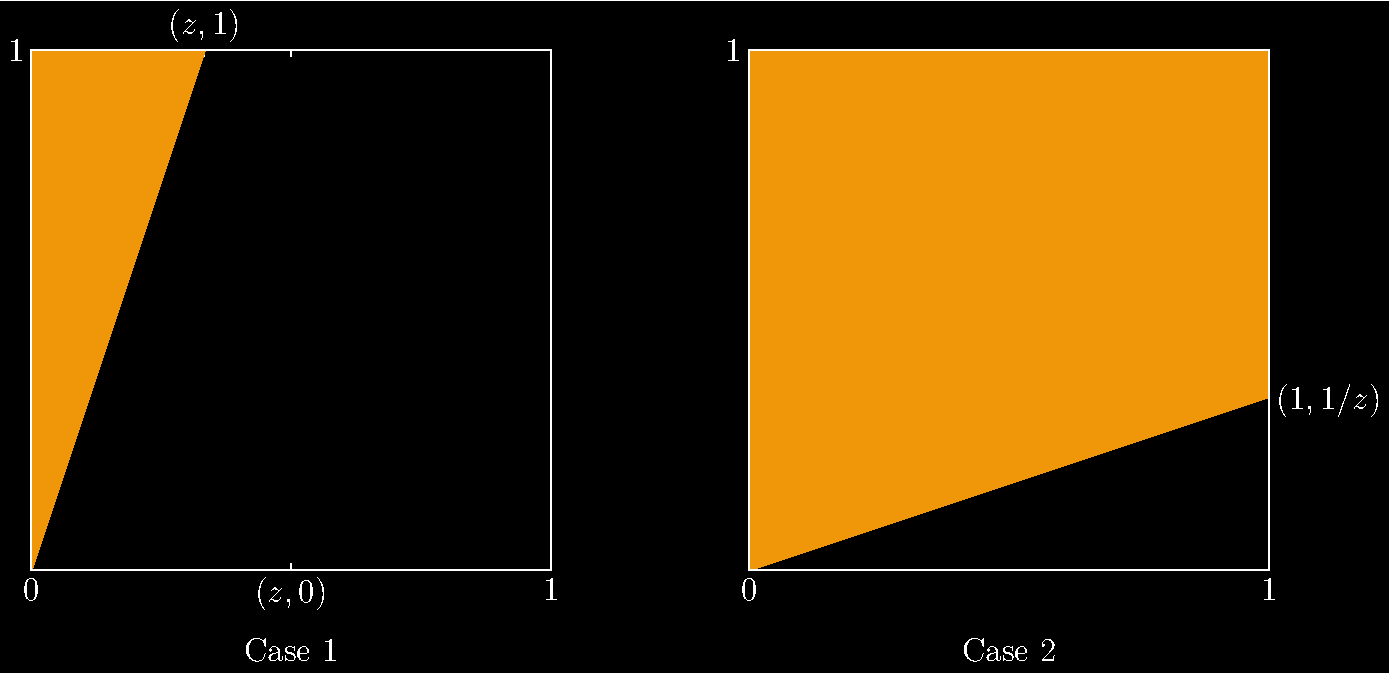
\includegraphics[width=1.0\textwidth]{chap2/chap2ex20ii.eps}
\end{center}

with \textsf{CDF}
\[
	F_{Z}(z) = \begin{cases}
		0 & z < 0 \\
		\frac{z}{2} & 0 < z < 1 \\
		1 - \frac{1}{2z} & z > 1
	\end{cases}
\]
and following that, the \textsf{PDF}
\[
	f_{Z}(z) = \begin{cases}
		\frac{1}{2} & 0 < z < 1 \\
		\frac{1}{2z^{2}} & z > 1 \\
		0 & \text{otherwise}
	\end{cases}
\]
Once again, the theoretical and the empirical align:
\begin{center}
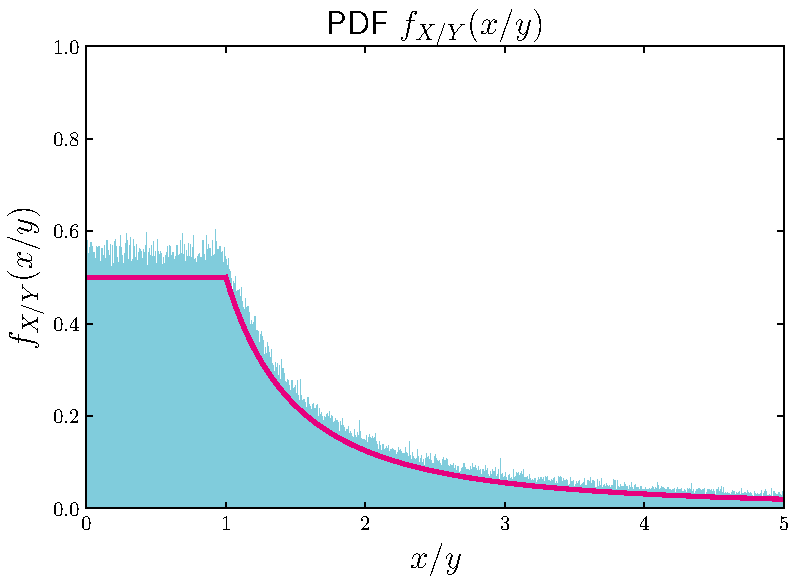
\includegraphics[width=1.0\textwidth]{chap2/chap2ex20iv.eps}
\end{center}

% QUESTION 21
\qs{2.14.21}{Let \(X_{1},\dots,X_{n} \sim \Exp(\beta )\) be \textsf{IID}. Let \(Y = \max\{X_{1},\dots,X_{n}\}\). Find the \textsf{PDF} of \(Y\). Hint: \(Y \le y\) if and only if \(X_{i} \le y\) for \(i = 1,\dots,n\).}

Taking advantage of the hint and the \textsf{IID} random variables, observe that \(\Prob(Y \le y) = \prod_{i=1}^{n} \Prob(X_{i} \le y) \). The derivation is straightforward:
\begin{align*}
	F_{Y}(y) = \Prob(Y \le y) & = \prod_{i=1}^{n} \int^{y}_{0} \frac{1}{\beta }e^{-x_{i}/\beta } \ dx_{i}   \\
	 & = \prod_{i=1}^{n} (1 - e^{-y/\beta })  \\
	 & = (1 - e^{-y/\beta })^{n} \\
	\implies F'_{Y}(y) = f_{Y}(y) = \frac{d }{d y} (1 - e^{-y/\beta })^{n} & = \boxed{\frac{n}{\beta } e^{-y/\beta }(1 - e^{-y/\beta })^{n-1}}
\end{align*}

\section{Chapter 3: Expectation}

\subsection*{Import Packages}

Please see the associated GitHub repo for all code and comments to simulations. [LINK HERE]

\begin{python}
import numpy as np
from numpy.random import choice
import random
import statistics
import matplotlib.pyplot as plt
import scienceplots
\end{python}

% QUESTION 1
\qs{3.8.1}{Suppose we play a game where we start with \(c\) dollars. On each play of the game you either double or halve your money, with equal probability. What is your expected fortune after \(n\) trials?}

By premise, \(\Prob(X = 2c) = 1/2, \Prob(X = \frac{1}{2}c) = 1/2\). By definition of expectation, we have
\[
	\E(X) = 2c \left( \frac{1}{2} \right) + \frac{1}{2}c \left( \frac{1}{2} \right) = \boxed{\frac{5}{4}c} 
\]

Simulating the money game, we find:

\begin{python}
def moneygame(c):
    flip = random.randint(0,1) 
    if flip == 0:
        c = 0.5*c
    else:
        c = 2*c
    return c;

c = 1
n = 5000

def runs(n):
    expectations = []
    for j in range(1,n+1):
        trials = []
        for i in range(1,j+1):
            trials.append(moneygame(c))
        mean = sum(trials)/len(trials)
        expectations.append(mean)
    return expectations;
\end{python}

\begin{center}
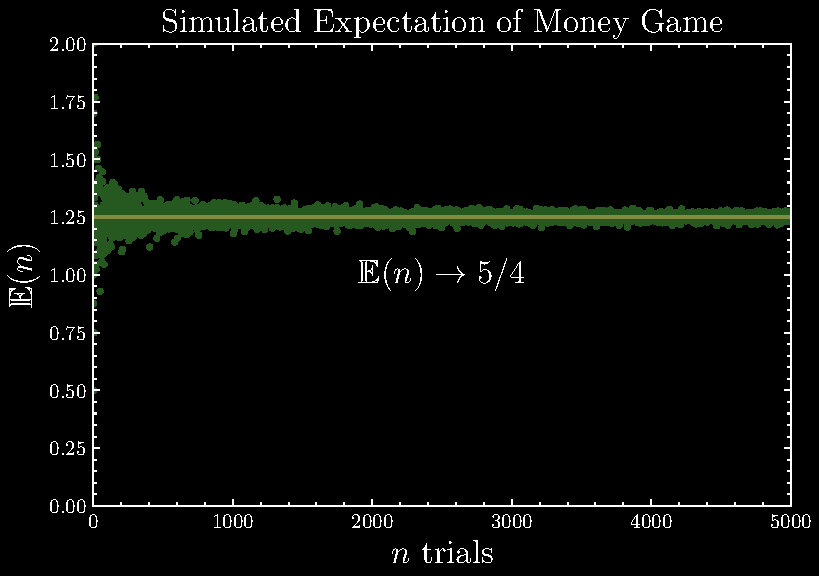
\includegraphics[width=1.0\textwidth]{chap3/chap3ex1.eps}
\end{center}

% QUESTION 2
\qs{3.8.2}{Show that \(\var(X) = 0 \) if and only if there is a constant \(c\) such that \(\Prob(X = c) = 1\).}
\begin{proof}[Proof] 
\(( \implies )\) Let \(\var(X) = 0\). Since \(\var(X) = \int (x - \mu)^{2}  \ dF(x) \), we must have \(x = \mu\). Then \(\Prob(X = \mu) = 1\).\vspace{12pt}
\par \((\impliedby)\) Let \(\Prob(X = c) = 1\). Then \(\E(X) = c\) and \(\E(X^{2}) = c^{2}\). Then \(\var(X) = \E(X^{2}) - \E(X)^{2} = c^{2} - c^{2} = 0\).
\end{proof}

% QUESTION 3
\qs{3.8.3}{Let \(X_{1},\dots,X_{n} \sim \Uniform(0,1)\) and let \(Y_{n} = \max\{X_{1},\dots,X_{n}\}\). Find \(\E(Y_{n})\).}

Assume \textsf{IID} standard uniform variables. Note that \(Y_{n} \le y\) if and only if \(X_{1},\dots,X_{n} \le y\). We can derive
\begin{align*}
	F_{Y_{n}}(y) & = \Prob(Y_{n} \le y) \\
	 & = \prod_{i=1}^{n} \Prob(X_{i} \le y)  \\
	 & = \prod_{i=1}^{n} \int^{y}_{0}  \ dx_{i} \\
	 & = y^{n}
\end{align*}
Then the \textsf{PDF} is
\[
	F_{Y_{n}}'(y) = f_{Y_{n}}(y) = ny^{n-1}
\]
and the expectation is
\[
	\E(Y_{n}) = \int^{1}_{0} ny^{n} \ dy = \boxed{\frac{n}{n+1}} 
\]

% QUESTION 4
\qs{3.8.4}{A particle starts at the origin of the real line and moves along the line in jumps of one unit. For each jump the probability is \(p\) that the particle will jump one unit to the left and the probability is \(1-p\) that the particle will jump one unit to the right. Let \(X_{n}\) be the position of the particle after \(n\) units. Find \(\E(X_{n})\) and \(\var(X_{n})\). (This is known as a \textbf{random walk}.)}

We define \(X\) as
\[
	X = \begin{cases}
		+1 & 1 - p \\
		-1 & p \\
	\end{cases}
\]
After one jump, 
\begin{align*}
	\E(X_{i}) & = 1(1-p) + (-1)p = 1 - 2p \\
	\E(X_{i}^{2}) & = 1 - p + p = 1 \\ 
	\var(X_{i}) & = \E(X_{i}^{2}) - \E(X_{i})^{2} = 1 - (1-2p)^{2} = 4(p - p^{2})
\end{align*}
After \(n\) jumps, assuming independence of each jump,
\begin{align*}
	\E \left( \sum_{}^{n} X_{i} \right)  & = \sum_{}^{n} \E(X_{i}) = \boxed{n(1-2p)} \\
	\var \left( \sum_{}^{n} X_{i} \right)  & = \sum_{}^{n} \var(X_{i}) = \boxed{4n(p-p^{2})} \\ 
\end{align*}

We can simulate some random walks for \(p = 0.5\):

\begin{python}
q = 0.5

def randomwalk(q):
    step = [-1,1]
    randomStep = choice( 
        step, 1, p=[q, 1-q])
    return randomStep.tolist()[0]

def trials(n): 
    record = []
    position = 0
    for i in range(1,n+1):
        position = position + randomwalk(q)
        record.append(position)
    return position, record;

def multiplewalks(k,n):
    walklist = []
    for i in range(1,k+1):
        trials(n)
        walklist.append(trials(n)[1])
    return walklist;

k = 5
n = 10000
\end{python}

\begin{center}
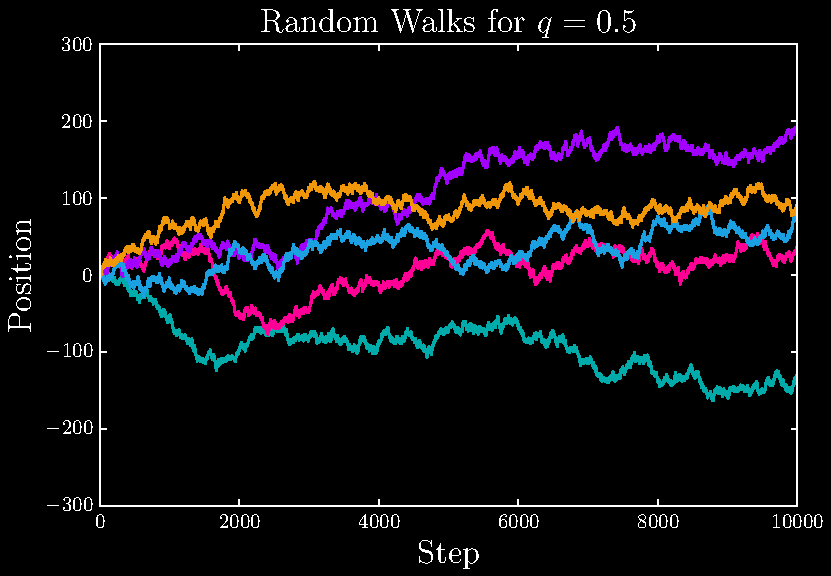
\includegraphics[width=1.0\textwidth]{chap3/chap3ex4i.eps}
\end{center}

Empirically simulating the expectation and variance for \(n\) steps also brings us quite close to our derived theoretical values:

\begin{python}
def trials(n):
    record = []
    position = 0
    for i in range(1,n+1):
        position = position + randomwalk(q)
    return position;

n = 10000
lastposition = []
for i in range(1, n+1):
    lastposition.append(trials(n))

e = statistics.mean(lastposition)
v = statistics.variance(lastposition)
\end{python}

\begin{center}
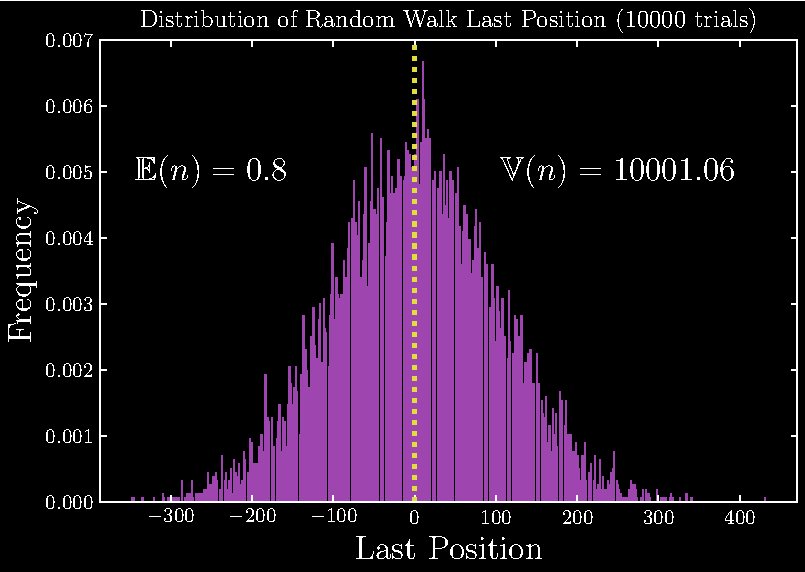
\includegraphics[width=1.0\textwidth]{chap3/chap3ex4ii.eps}
\end{center}

% QUESTION 5
\qs{3.8.5}{A fair coin is tossed until a head is obtained. What is the expected number of tosses that will be required?}

In general, for a coin in which a head is obtained with probability \(p\), we can model the expected number of tosses until we get a head with the geometric distribution:
\[
	\Prob(X = k) = p(1-p)^{k-1}
\]
Deriving the first moment, we first write the \textsf{MGF} (with \(q = 1-p)\)
\begin{align*}
	\psi_{X}(t) & \sum_{x} e^{tx}pq^{x-1} \\
	 & = p(e^{t} + qe^{2t} + q^{2}e^{3t} + \cdots ) \\ 
	 & = pe^{t}(1 + qe^{t} + q^{2}e^{2t} + \cdots ) \\
	 & = \frac{pe^{t}}{1 -qe^{t}}
\end{align*}
Differentiating gives us
\[
	\psi'_{X}(t) = pe^{t}(1-qe^{t})^{-1} - pe^{t}(-qe^{t})(1-qe^{t})^{-2}
\]
And setting \(t=0\) gives us
\begin{align*}
	\psi'_{X}(0) & p(1-q)^{-1} - p(-q)(1-q)^{-2}  \\
	 & = \frac{1}{p} 
\end{align*}
For \(p = 1/2\), \(\E(X) = \frac{1}{1/2} = \boxed{2}\). Simulating gives us the desired expectation:

\begin{python}
def cointoss(): 
    tosses, heads = [], 0
    while (heads < 1):
        flip = random.randint(0,1)
        if (flip == 0):
            tosses.append('Heads')
            heads = tosses.count('Heads')
        else:
            tosses.append('Tails')
    return len(tosses);

def empirical(n): 
    numtosses, probs = [], []
    for i in range(0,n):
        numtosses.append(cointoss())
    for x in np.unique(numtosses): 
        probs.append((x, numtosses.count(x)))
    return numtosses;

def trials(n): 
    trials = []
    for i in range(1,n+1):
        trials.append(statistics.mean(empirical(i)))
    return trials;

n = 10000
\end{python}

\begin{center}
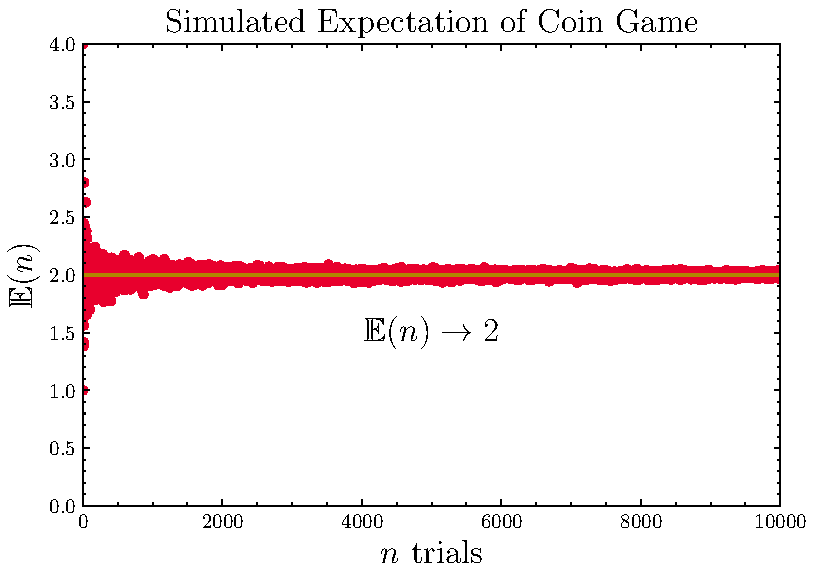
\includegraphics[width=1.0\textwidth]{chap3/chap3ex5.eps}
\end{center}

% QUESTION 6
\qs{3.8.6}{Prove Theorem 3.6 for discrete random variables.}
\begin{proof}[Proof] 
Let \(Y = r(X)\). We make no assumption about whether \(r\) is a bijection, namely if it has an inverse. Therefore, it is possible for multiple values of \(X = x\) to map to the same \(Y = y \). For instance, if \(Y = r(X) = X^{2}\), then \(X = 1\) and \(X = -1\) map to \(Y = 1\), and we have \(\Prob(Y = 1) = \Prob(X = 1) + \Prob(X = -1)\).

From the definition of expectation, we have
\[
	\E(Y) = \sum_{i} y_{i} \Prob(Y = y_{i})
\]
Now, \(\Prob(Y = y_{i})\) is equal to the sum of the probabilities of \(X\) taking on all values \(x_{j}\) such that \(y_{i} = g(X = x_{j})\). In other words,
\[
	\Prob(Y = y_{i}) = \sum_{j:y_{i}= g(x_{j})} \Prob(X = x_{j}) = \Prob(X = x)
\]
Thus we can conclude with
\begin{align*}
	 & = \sum_{i} y_{i} \sum_{j: y_{i} = g(x_{j})} \Prob(X = x_{j}) \\
	 & = \sum g(x)\Prob(X = x) \\
	 & = \sum g(x) f_{X}(x)
\end{align*}
\end{proof}

% QUESTION 7
\qs{3.8.7}{Let \(X\) be a continuous random variable with \textsf{CDF} \(F\). Suppose that \(\Prob(X > 0) = 1\) and that \(\E(X)\) exists. Show that \(\E(X) = \int^{\infty}_{0} \Prob(X > x) \ dx \).

Hint: Consider integrating by parts. The following fact is helpful: if \(\E(X)\) exists then \(\lim_{x \to \infty} x[1 - F(x)] = 0.\)}
\begin{proof}[Proof] 
By definition of expectation for a continuous random variable,
\[
	\E(X) = \int^{\infty}_{0} x f_{X}(x) \ dx 
\]
Proceeding with integration by parts, let \(\mu = x, dv = f_{X}(x) dx\). Then \(du = dx, v = F_{X}(x)\). We continue with
\begin{align*}
	 & = x F_{X}(x) \bigg| ^{\infty}_{0} - \int^{\infty}_{0} F_{X}(x) \ dx  \\
	 & = x \bigg| ^{\infty}_{0} - \int^{\infty}_{0} F_{X}(x) \ dx  \\ 
	 & = \int^{\infty}_{0}  \ dx - \int^{\infty}_{0} F_{X}(x) \ dx \\  
	 & = \int^{\infty}_{0} [1 - F_{X}(x)] \ dx \\
	 & = \int^{\infty}_{0} \Prob(X > x) \ dx 
\end{align*}
with the second equality following from the fact that \(\lim_{x \to \infty} x[1 - F_{X}(x)] = 0\), implying that \(\lim_{x \to \infty} x = \lim_{x \to \infty} x F_{X}(x) \). 
\end{proof}

\newpage
% QUESTION 8
\qs{3.8.8}{Prove Theorem 3.17.}
\thm{(Wasserman 3.17)}{Let \(X_{1},\dots,X_{n}\) be \textsf{IID} and let \(\mu = \E(X_{i}), \sigma^{2} = \var(X_{i}) \). Then
\[
	\E(\overline{X}_{n}) = \mu, \quad \var(\overline{X}_{n}) = \frac{\sigma^{2}}{n} \quad \text{and} \quad \E(S^{2}_{n}) = \sigma^{2}.
\]}
\begin{proof}[Proof] 
Use the fact that the \(X_{i}\)'s are \textsf{IID}.
\begin{align*}
	\E(\overline{X}_{n}) & = \E \left( \frac{1}{n} \sum_{i=}^{n} X_{i} \right)  \\
	 & = \frac{1}{n} \E \left( \sum_{i=1}^{n} X_{i} \right)  \\ 
	 & = \frac{1}{n} \sum_{i=1}^{n} \E(X_{i}) \\
	 & = \frac{1}{n} (n \mu) \\
	 & = \boxed{\mu} \\
	\var(\overline{X}_{n}) & = \var \left( \frac{1}{n} \sum_{i=1}^{n} X_{i} \right) \\
	 & = \sum_{i=1}^{n} \frac{1}{n^{2}} \var(X_{i}) \\
	 & = \frac{1}{n^{2}} (n \sigma^{2}) \\
	 & = \boxed{\frac{\sigma^{2}}{n}} 
\end{align*}
\begin{align*}
	\E(S^{2}_{n}) & = \E \left( \frac{1}{n-1} \sum_{i=1}^{n} (X_{i} - \overline{X}_{n})^{2} \right)  \\
	 & = \E \left( \frac{1}{n-1} \sum_{i=1}^{n} (X_{i}^{2} - 2X_{i}\overline{X}_{n} + \overline{X}_{n}^{2}) \right)  \\ 
	 & = \E \left( \frac{1}{n-1} \sum_{i=1}^{n} X_{i}^{2} - n \overline{X}_{n}^{2} \right) \\
	 & = \frac{1}{n-1} \left( \sum_{i=1}^{n} \E(X_{i}^{2}) - n \E(\overline{X}_{n}^{2}) \right) \\
	 & = \frac{1}{n-1}(n(\sigma^{2} + \mu^{2})) - \frac{1}{n-1}\frac{1}{n}(n(n-1) \mu^{2} + n(\sigma^{2} + \mu^{2})) \\
	 & = \frac{1}{n-1}(n(\sigma^{2} + \mu^{2})) - \frac{1}{n-1}(n \mu^{2} + \sigma^{2}) \\
	 & = \frac{n \sigma^{2} - \sigma^{2}}{n-1} \\
	 & = \boxed{\sigma^{2}}
\end{align*}
\end{proof}

% QUESTION 9
\qs{3.8.9}{\textsf{(Computer Experiment.)} Let \(X_{1}, X_{2}, \dots, X_{n}\) be \(N(0,1)\) random variables and let \(\overline{X}_{n} = n^{-1} \sum_{i=1}^{n} X_{i}\). Plot \(\overline{X}_{n}\) versus \(n\) for \(n = 1, \dots, 10,000\). Repeat for \(X_{1}, X_{2},\dots, X_{n} \sim \) Cauchy. Explain why there is such a difference.}

We can code our functions to generate \(\overline{X}_{n}\) for the \(N(0,1)\) and Cauchy distributions as follows:

\begin{python}
def normal(n):
    normalmeans = []
    for i in range(1,n+1):
        normalmeans.append(statistics.mean(np.random.normal(0,1,i)))
    return normalmeans;

def cauchy(n):
    cauchymeans = []
    for i in range(1,n+1):
        cauchymeans.append(
		statistics.mean(np.random.standard_cauchy(i)))
    return cauchymeans;

n = 10000
\end{python}

The simulations yield:

\begin{center}
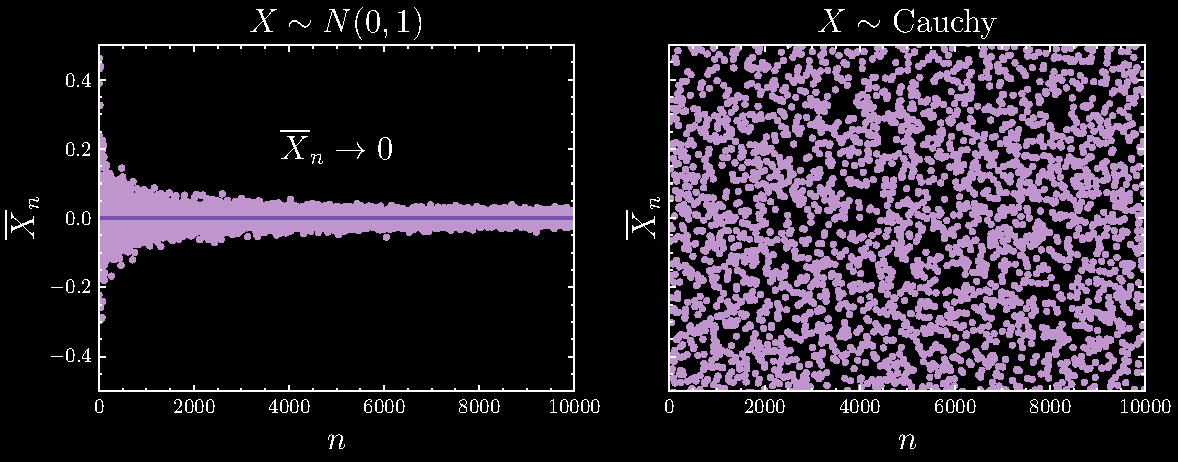
\includegraphics[width=1.0\textwidth]{chap3/chap3ex9.eps}
\end{center}

A striking comparison! Qualitatively, the standard normal and standard Cauchy distributions look to be quite similar. But notably, the latter \textit{has no mean}. Given the \textsf{PDF}
\[
	f_{Z}\left( z \right) = \frac{1}{\pi (1 + z^{2})}, \quad z \in \mathbb{R}
\]
which is generated by finding the distribution of \(Z = X/Y\) for \(X,Y \sim N(0, \sigma^{2})\), the expectation \(\E\left( Z \right)\) turns out to diverge.

% QUESTION 10
\qs{3.8.10}{Let \(X \sim N(0,1)\) and let \(Y = e^{X}\). Find \(\E(Y)\) and \(\var(Y)\).}

By the Law of the Unconscious Statistician, we have
\begin{align*}
	\E(Y) & = \frac{1}{\sqrt{2 \pi }} \int^{\infty}_{-\infty} e^{x} e^{-x^{2}/2} \ dx  \\
	 & = \frac{1}{\sqrt{2 \pi }} \int^{\infty}_{-\infty} e^{-x^{2}/2 + x} \ dx  \\ 
\end{align*}
Using the identity
\[
	\int^{\infty}_{-\infty} e^{-ax^{2} + bx} \ dx = e^{b^{2}/4a} \sqrt{\frac{\pi }{a}}
\]
with \(a = b = 1\), we can conclude
\[
	\E(Y) = \frac{1}{\sqrt{2 \pi }} e^{1/2} \sqrt{2 \pi } = \boxed{e^{1/2}}
\]
Similarly, we calculate \(\E(Y^{2})\):
\begin{align*}
	\E(Y^{2}) & = \frac{1}{\sqrt{2 \pi }} \int^{\infty}_{-\infty} e^{2x} e^{-x^{2}/2} \ dx  \\
	 & = \frac{1}{\sqrt{2 \pi }} \int^{\infty}_{-\infty} e^{-x^{2}/2 + 2x} \ dx  \\ 
	 & = e
\end{align*}
and derive
\[
	\var(Y) = \E(Y^{2}) - \E(Y)^{2} = \boxed{e^{2} - e}
\]

Simulating, we get

\begin{python}
n = 10000 

x = np.random.normal(0,1,n) # normal samples
y = np.exp(x) # exponential transformation
meany = round(statistics.mean(y),2)
vary = round(statistics.variance(y),2)
\end{python}

\begin{center}
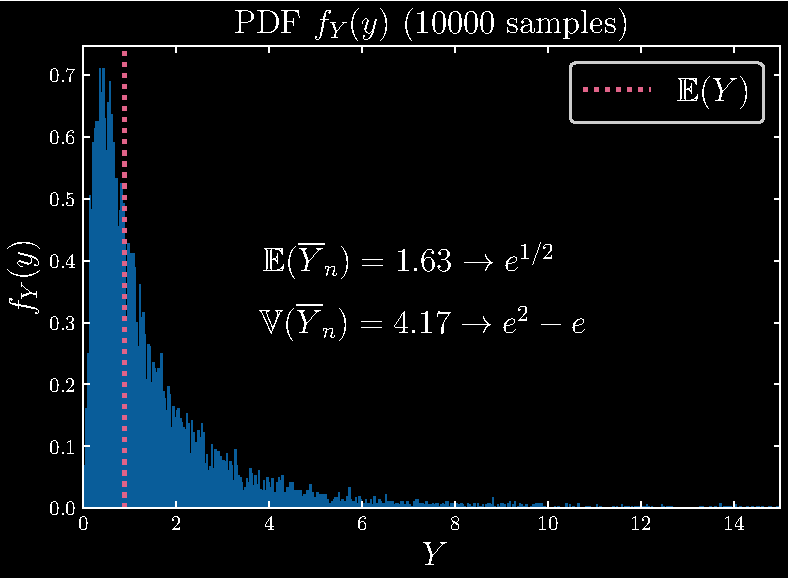
\includegraphics[width=1.0\textwidth]{chap3/chap3ex10.eps}
\end{center}

\newpage
% QUESTION 11
\qs{3.8.11}{\textsf{(Computer Experiment: Simulating the Stock Market.)} Let \(Y_{1}, Y_{2},\dots\) be independent random variables such that \(\Prob(Y_{i} = 1) = \Prob\left( Y_{i} = -1 \right) = 1/2\). Let \(X_{n} = \sum_{i=1}^{n} Y_{i}\). Think of \(Y_{i} = 1\) as "the stock price increased by one dollar," \(Y_{i} = -1\) as "the stock price decreased by one dollar," and \(X_{n}\) as the value of the stock on day \(n\).
\begin{enumerate}[label=(\alph*)]
	\item Find \(\E(X_{n})\) and \(\var(X_{n})\).
	\item Simulate \(X_{n}\) and plot \(X_{n}\) versus \(n\) for \(n = 1, 2, \dots, 10,000\). Repeat the whole simulation several times. Notice two things. First, it's easy to "see" patterns in the sequence even though it is random. Second, you will find that the four runs look very different even though they were generated the same way. How do the calculations in (a) explain the second observation?
\end{enumerate}}

(a) The expectation and variance are derived as
\begin{align*}
	\E\left( Y_{i} \right) & = 1 \cdot \frac{1}{2} - 1 \cdot \frac{1}{2} = 0\\
	\implies \E\left( X_{n} \right) & = \E\left( \sum_{i=1}^{n} Y_{i} \right) = \boxed{0} \\ 
	\E\left( Y^{2}_{i} \right) & = 1 \cdot \frac{1}{2} + 1 \cdot \frac{1}{2} = 1 \\
	\var\left( Y_{i} \right) & = \E\left( Y^{2}_{i} \right) - \E\left( Y_{i} \right)^{2} = 1 \\
	\implies \var\left( X_{n} \right) & = \var\left( \sum_{i=1}^{n} Y_{i} \right) = \boxed{n}
\end{align*}

\par (b) Refer to exercise 3.8.4, as this exercise is a special case of the random walk where \(p = 0.5\). The intuition for why the paths diverge at increasing number of steps \(n\) is because of the path-dependency of the movement of the sequence -- the position in the random walk or the stock price is contingent on what came before it -- and that the variance is dependent on \(n\) (in fact it is \(n\) itself). For high \(n\), the larger the spread of \(X_{n}\). 

\newpage
% QUESTION 12
\qs{3.8.12}{Prove the formulas given in the table at the beginning of Section 3.4 for the Bernoulli, Poisson, Uniform, Exponential, Gamma, and Beta. Here are some hints. For the mean of the Poisson, use the fact that \(e^{a} = \sum_{x=0}^{\infty} a^{x}/x!\). To compute the variance, first compute \(\E(X(X-1))\). For the mean of the Gamma, it will help to multiply and divide by \(\Gamma(\alpha + 1)/\beta^{\alpha +1}\) and use the fact that a Gamma density integrates to 1. For the Beta, multiply and divide by \(\Gamma(\alpha + 1) \Gamma(\beta) / \Gamma(\alpha + \beta + 1)\).}
\begin{proof}[Proof] 
\underline{Bernoulli}
\begin{align*}
	\E(X) & = 1 \cdot \Prob(X = 1) + 0 \cdot \Prob(X = 0) = \boxed{p} \\
	\E(X^{2}) & = 1^{2} \cdot \Prob(X = 1) + 0^{2} \cdot \Prob(X = 0) = p \\ 
	\var(X) & = \E(X^{2}) - \E(X)^{2} = p - p^{2} = \boxed{p(1-p)}
\end{align*}

\underline{Poisson}
Using the infinite sum definition of \(e^{x}\):
\[
	e^{x} = \sum_{k=1}^{\infty} \frac{x^{k-1}}{(k-1)!}
\]
we can derive
\begin{align*}
	\E(X) & = \sum_{x=0}^{\infty} xe^{-\lambda } \frac{\lambda^{x}}{x!} \\
	 & = \sum_{x=1}^{\infty} e^{-\lambda } \frac{\lambda^{x}}{(x-1)!} \\ 
	 & = \lambda e^{-\lambda } \sum_{x=1}^{\infty} \frac{\lambda^{x-1}}{(x-1)!} \\
	 & = \lambda e^{-\lambda }e^{\lambda } \\
	 & = \boxed{\lambda } \\
	\E(X(X-1)) & = \sum_{x=0}^{\infty} x(x-1) e^{-\lambda } \frac{\lambda^{x}}{x!} \\
	 & = \lambda \sum_{x=1}^{\infty} (x-1) e^{-\lambda } \frac{\lambda^{x-1}}{(x-1)!} \\
	 & = \lambda^{2}
\end{align*}
which implies \(\E(X^{2}) = \lambda^{2} + \lambda \), and in turn
\[
	\var(X) = \E(X^{2}) - \E(X)^{2} = \lambda^{2} + \lambda - \lambda^{2} = \boxed{\lambda }
\]

\underline{Uniform}
\begin{align*}
	\E(X) & = \int^{b}_{a} x \left( \frac{1}{b-a} \right)  \ dx  \\
	      & = \boxed{\frac{a + b}{2}} \\
	\E(X^{2}) & = \int^{b}_{a} x^{2} \left( \frac{1}{b-a} \right)  \ dx \\
	      & = \frac{a^{2} + ab + b^{2}}{3} \\
	\var(X) & = \E(X^{2}) - \E(X)^{2} \\
	      & = \frac{a^{2} + ab+ b^{2}}{3} - \left( \frac{a+b}{2} \right)^{2} \\
	      & = \boxed{\frac{(b-a)^{2}}{12}}
\end{align*}

\underline{Exponential}
We will have to carry out this integration by parts. Let \(\mu = x, dv = \exp(-x/\beta ) dx\). Then \(du = dx, v = -\beta \exp(-x/\beta )\).
\begin{align*}
	\E(X) & = \frac{1}{\beta } \int^{\infty}_{0} x \exp(-x/\beta ) \ dx  \\
	 & = \frac{1}{\beta } \left( -\beta x \exp(-x/\beta ) \bigg|^{\infty}_{0} + \int^{\infty}_{0} \beta \exp(-x/\beta ) \ dx  \right)   \\
	 & = -\beta \exp(-x/\beta ) \bigg| ^{\infty}_{0} \\
	 & = \boxed{\beta }
\end{align*}
To calculate \(\E(X^{2})\), let \(\mu = x, dv = x \exp(-x/\beta ) dx\), then \(du = dx, v = -(\beta x + \beta^{2}) \exp(-x/\beta )\).
\begin{align*}
	\E(X^{2}) & = \frac{1}{\beta } \int^{\infty}_{0} x^{2} \exp(-x/\beta ) \ dx  \\
	 & = \frac{1}{\beta } \bigg( -(\beta x + \beta^{2}) x \exp(-x/\beta ) \bigg|^{\infty}_{0} \\
	 & \quad + \beta \int^{\infty}_{0} x \exp(-x/\beta ) \ dx + \beta^{2} \int^{\infty}_{0} \exp(-x/\beta ) \ dx   \bigg)  \\ 
	 & = \int^{\infty}_{0} x \exp(-x/\beta ) \ dx + \beta \int^{\infty}_{0} \exp(-x/\beta ) \ dx \\
	 & = \beta^{2} + \beta^{2} \\
	 & = 2 \beta^{2}
\end{align*}
and now the variance:
\[
	\var(X) = \E(X^{2}) - \E(X)^{2} = \boxed{\beta^{2}}
\]

\underline{Gamma}
Use the identity
\[
	\Gamma(\alpha + 1) = \alpha \int^{\infty}_{0} t^{\alpha - 1}e^{-t} \ d \alpha = \alpha \Gamma(\alpha) 
\]
Then we can calculate
\[
	\E(X) = \frac{1}{\beta^{\alpha } \Gamma(\alpha)} \int^{\infty}_{0} x^{\alpha } e^{-x/\beta } \ dx
\]
Let \(X = \beta y\). Then \(dx = \beta dy\). (Use this substitution for \(\E(X^{2})\) too.)
\begin{align*}
	 & = \frac{1}{\beta^{\alpha } \Gamma(\alpha )} \int^{\infty}_{0} (\beta y)^{\alpha } e^{-y} \beta  \ dy  \\
	 & = \beta \frac{\Gamma(\alpha +1)}{\Gamma(\alpha)} \\
	 & = \beta \frac{\alpha \Gamma(\alpha )}{\Gamma(\alpha )} \\
	 & = \boxed{\alpha \beta } \\
	\E(X^{2}) & = \frac{1}{\beta^{\alpha } \Gamma(\alpha )} \int^{\infty}_{0} x^{\alpha + 1} e^{-x/\beta } \ dx \\
	 & = \frac{1}{\beta^{\alpha } \Gamma(\alpha )} \int^{\infty}_{0} (\beta y)^{\alpha + 1} e^{-y} \beta  \ dy \\
	 & = \beta^{2} \frac{\Gamma(\alpha + 2)}{\Gamma(\alpha )} \\
	 & = \beta^{2} \frac{(\alpha + 1) \alpha  \Gamma(\alpha)}{\Gamma(\alpha)} \\
	 & = \alpha (\alpha + 1) \beta^{2} \\
	\var(X) & = \E(X^{2}) - \E(X)^{2} \\
	 & = \alpha (\alpha + 1) \beta^{2} - (\alpha \beta )^{2} \\
	 & = \boxed{\alpha \beta^{2}}
\end{align*}

\underline{Beta}
\begin{align*}
	\E(X) & = \frac{\Gamma (\alpha + \beta )}{\Gamma(\alpha ) \Gamma(\beta )} \int^{1}_{0} x^{\alpha } (1-x)^{\beta -1} \ dx  \\
	 & = \frac{\Gamma(\alpha + \beta)}{\Gamma(\alpha ) \Gamma(\beta )} \frac{\Gamma(\alpha + 1) \Gamma(\beta ) / \Gamma( \alpha + \beta + 1)}{\Gamma(\alpha + 1) \Gamma(\beta) / \Gamma(\alpha + \beta + 1)} \int^{1}_{0} x^{\alpha } (1-x)^{\beta - 1} \ dx  \\ 
	 & = \frac{\Gamma(\alpha + \beta) \Gamma(\alpha + 1) \Gamma(\beta)}{\Gamma(\alpha) \Gamma(\beta) \Gamma(\alpha + \beta + 1)} \\
	 & = \frac{\alpha \Gamma(\alpha) \Gamma(\alpha + \beta)}{(\alpha + \beta) \Gamma(\alpha) \Gamma(\alpha + \beta)} \\
	 & = \boxed{\frac{\alpha }{\alpha + \beta }} \\
	\E(X^{2}) & = \frac{\Gamma(\alpha + \beta)}{\Gamma(\alpha) \Gamma(\beta)} \int^{1}_{0} x^{\alpha + 1} (1-x)^{\beta - 1} \ dx \\
	 & = \frac{\Gamma(\alpha + \beta )}{\Gamma(\alpha) \Gamma(\beta)} \frac{\Gamma(\alpha +2) \Gamma(\beta) / \Gamma(\alpha + \beta + 2)}{\Gamma(\alpha + 2) \Gamma(\beta) / \Gamma(\alpha + \beta + 2)} \int^{1}_{0} x^{\alpha + 1} (1-x)^{\beta - 1} \ dx \\
	 & = \frac{\Gamma(\alpha + \beta) \Gamma(\alpha + 2) \Gamma(\beta)}{\Gamma(\alpha) \Gamma(\beta) \Gamma(\alpha + \beta + 2)} \\
	 &= \frac{\alpha (\alpha + 1) \Gamma(\alpha) \Gamma(\alpha + \beta)}{(\alpha + \beta) (\alpha + \beta + 1) \Gamma(\alpha) \Gamma(\alpha + \beta)} \\
	 & = \frac{\alpha (\alpha + 1)}{(\alpha + \beta )(\alpha + \beta + 1)} \\
	\var(X) & = \E(X^{2}) - \E(X)^{2} \\
	 & = \frac{\alpha (\alpha + 1)}{(\alpha + \beta)(\alpha + \beta + 1)} - \left( \frac{\alpha }{\alpha + \beta } \right)^{2} \\
	 & = \boxed{\frac{\alpha \beta }{(\alpha + \beta)^{2} (\alpha + \beta + 1)}}
\end{align*}
\end{proof}

\newpage
% QUESTION 13
\qs{3.8.13}{Suppose we generate a random variable \(X\) in the following way. First we flip a fair coin. If the coin is heads, take \(X\) to have a \(\Uniform(0,1)\) distribution. If the coin is tails, take \(X\) to have a \(\Uniform(3,4)\) distribution.
\begin{enumerate}[label=(\alph*)]
	\item Find the mean of \(X\).
	\item Find the standard deviation of \(X\).
\end{enumerate}}

(a) If heads, then \(X \sim \Uniform(0,1)\), and if tails, \(X \sim \Uniform(3,4)\). By the definition of expectation:
\begin{align*}
	\E(X) & = \frac{1}{2} \left( \int^{1}_{0} x \ dx + \int^{4}_{3} x \ dx   \right)  \\
	 & = \frac{1}{2} \left( \frac{1}{2} + \frac{7}{2} \right)  \\ 
	 & = \boxed{2}
\end{align*}
\par (b) By definition, the standard deviation \(\sd(X)\) is \(\sqrt{\var(X)}\). Calculate
\begin{align*}
	\E(X^{2}) & = \frac{1}{2} \left( \int^{1}_{0} x^{2} \ dx + \int^{4}_{3} x^{2} \ dx   \right)  \\
	 & = \frac{1}{2} \left(\frac{1}{3} + \frac{37}{3} \right)  \\ 
	 & = \frac{19}{3} \\
	\var(X) & = \E(X^{2}) - \E(X)^{2} \\
	 & = \frac{19}{3} - \frac{12}{3} \\
	 & = \frac{7}{3} \\
	\implies \sd(X) & = \boxed{\sqrt{\frac{7}{3}}}
\end{align*}

The simulation gives us:

\begin{python}
def coingame():
    flip = random.randint(0,1) 
    if flip == 0:
        x = np.random.uniform(0,1)
    else:
        x = np.random.uniform(3,4)
    return x;

def samples(n):
    samples = []
    for i in range(1,n+1):
        samples.append(coingame())
    return samples;

n = 100000

exp = round(statistics.mean(samples(n)),3)
sd = round(np.sqrt(statistics.variance(samples(n))),3)
print('The expected value is ', exp, ' 
      and the standard deviation is ', sd)
\end{python}

The expected value is  \(2.004\)  and the standard deviation is  \(1.528\). The distribution looks like:

\begin{center}
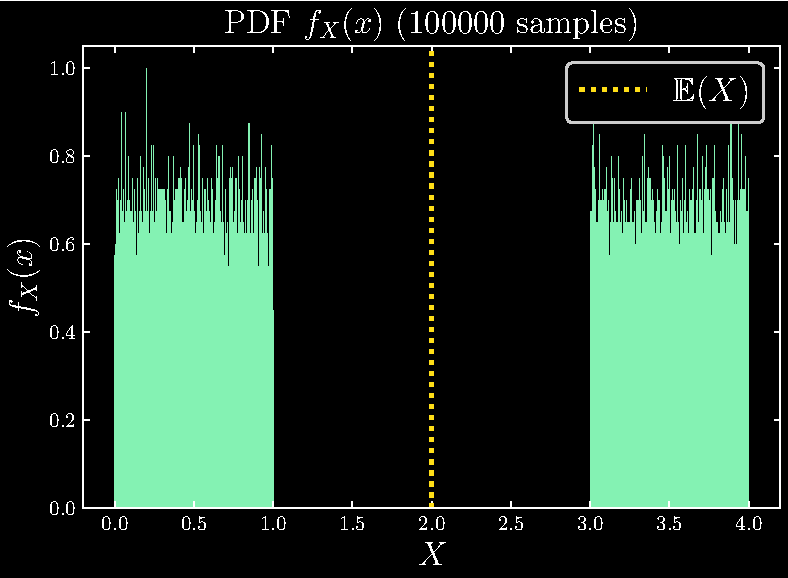
\includegraphics[width=1.0\textwidth]{chap3/chap3ex13.eps}
\end{center}

% QUESTION 14
\qs{3.8.14}{Let \(X_{1},\dots, X_{m}\) and \(Y_{1}, \dots, Y_{n}\) be random variables and let \(a_{1},\dots, a_{m}\) and \(b_{1},\dots, b_{n}\) be constants. Show that
\[
	\cov \left( \sum_{i=1}^{m} a_{i} X_{i}, \sum_{j=1}^{n} b_{j} Y_{j} \right) = \sum_{i=1}^{m} \sum_{j=1}^{n} a_{i} b_{j} \cov(X_{i}, Y_{j}).
\]}
\begin{proof}[Proof] 
By definition of \(\cov(X,Y)\):
\[
	\cov(X,Y) = \E \left((X - \mu_{X})(Y - \mu_{Y}) \right) 
\]
First, we will calculate the means of the two sums.
\begin{align*}
	\E \left( \sum_{i=1}^{m} a_{i} X_{i} \right)  & = \sum_{i=1}^{m} a_{i} \E(X_{i}) = \sum_{i=1}^{m} a_{i} \mu_{X_{i}} \\
	\E \left( \sum_{j=1}^{n} b_{j} Y_{j} \right)  & = \sum_{j=1}^{n} b_{j} \E(Y_{j}) = \sum_{j=1}^{n} b_{j} \mu_{Y_{j}} \\ 
\end{align*}
Proceeding from the definition of covariance, we can continue to derive
\[
	\cov \left( \sum_{i=1}^{m} a_{i} X_{i}, \sum_{j=1}^{n} b_{j} Y_{j} \right) 
\]
\begin{align*}
	 & = \E \left( \left( \sum_{i=1}^{m} a_{i}X_{i} - \sum_{i=1}^{m} a_{i}\mu_{X_{i}} \right) \left( \sum_{j=1}^{n} b_{j}Y_{j} - \sum_{j=1}^{n} b_{j} \mu_{Y_{j}} \right)  \right)  \\
	 & = \E \left( \left( \sum_{i=1}^{m} a_{i} (X_{i} - \mu_{X_{i}}) \right) \left( \sum_{j=1}^{n} b_{j}(Y_{j} - \mu_{Y_{j}} \right)  \right)  \\ 
	 & = \E \left( a_{1}(X_{1} - \mu_{X_{1}}) \sum_{j=1}^{n} b_{j}(Y_{j} - \mu_{Y_{j}}) + \cdots + a_{n}(X_{n} - \mu_{X_{n}}) \sum_{j=1}^{n} b_{j} (Y_{j}-\mu_{Y_{j}}) \right) \\
	 & = \E(a_{1}(X_{1} - \mu_{X_{1}})b_{1}(Y_{1} - \mu_{Y_{1}}) + \cdots + a_{1}(X_{1} - \mu_{X_{1}}) b_{n}(Y_{n} - \mu_{Y_{n}}) + \cdots\\
	 & \qquad + a_{n}(X_{1} - \mu_{X_{1}}) b_{1}(Y_{1} - \mu_{Y_{1}}) + \cdots + a_{n} (X_{1} - \mu_{X_{1}}) b_{n}(Y_{n} - \mu_{Y_{n}})) \\
	 & = \sum_{i=1}^{m} \sum_{j=1}^{n} \E(a_{i}b_{j}(X_{i} - \mu_{X_{i}})(Y_{j} - \mu_{Y_{j}})) \\
	 & = \sum_{i=1}^{m} \sum_{j=1}^{n} a_{i}b_{j} \cov(X_{i},Y_{j})
\end{align*}
\end{proof}

% QUESTION 15
\qs{3.8.15}{Let
\[
	f_{X,Y}(x,y) = \begin{cases}
		\frac{1}{3}(x+y) & 0 \le x \le 1, 0 \le y \le 2 \\
		0 & \text{otherwise.} \\
	\end{cases}	
\]
Find \(\var(2X-EY+8)\).}
The two approaches to this problem are to either use the definition \(\var(X) = \E(X^{2}) - \E(X)^{2}\), or to derive the marginal densities and individually calculate the expectations and variances for \(X,Y\). The first is far shorter, but we will solve using both methods.

Given \(\var(2X - 3Y + 8)\), observe that this is equivalent to \(\var(2X - 3Y)\), using the fact that constant terms do not affect the variance of a sum of random variables. Therefore we calculate
\[
	\var(2X - 3Y) = \E((2X-3Y)^{2}) - \E(2X-3Y)^{2}
\]
\begin{align*}
	\E((2X-3Y)^{2}) & = \int^{2}_{0} \int^{1}_{0} (2x-3y)^{2} \frac{1}{3} (x+y) \ dx  \ dy = \frac{86}{9}  \\
	\E(2X-3Y) & = \int^{2}_{0} \int^{1}_{0} (2x-3y) \frac{1}{3}(x + y) \ dx  \ dy = -\frac{23}{9} \\ 
	\var(2X-3Y) & = \frac{86}{9} - \left( -\frac{23}{9} \right)^{2} \\
		    & = \boxed{\frac{245}{81}}
\end{align*}

For the second method, begin with deriving the marginal densities:
\begin{align*}
	f_{X}(x) & = \int^{2}_{0} \frac{1}{3}(x + y) \ dy = \frac{2}{3}(x+1), \quad 0 \le x \le 1 \\
	f_{Y}(y) & = \int^{1}_{0} \frac{1}{3}(x + y) \ dx = \frac{1}{3} \left( \frac{1}{2} + y \right), \quad 0 \le y \le 2  \\ 
\end{align*}
The constituent expectations for calculations down the line are
\begin{align*}
	\E(X) & = \int^{1}_{0} \frac{2}{3}(x^{2} + x) \ dx = \frac{5}{9}  \\
	\E(X^{2}) & = \int^{1}_{0} \frac{2}{3}(x^{3} + x^{2}) \ dx = \frac{7}{18} \\ 
	\E(Y) & = \int^{2}_{0} \frac{1}{3}\left( y^{2} + \frac{y}{2} \right)  \ dy = \frac{11}{9} \\
	\E(Y^{2}) & = \int^{2}_{0} \frac{1}{3} \left( y^{3} + \frac{y^{2}}{2} \right)  \ dy = \frac{16}{9} \\
	\E(XY) & = \int^{2}_{0} \int^{1}_{0} xy f_{X,Y}(x,y) \ dx  \ dy\\
	       & = \int^{2}_{0} \int^{1}_{0} \frac{1}{3} (x^{2}y + xy^{2} \ dx  \ dy = \frac{2}{3} \\ 
\end{align*}
For the last step, the desired variance is calculated as
\[
	\var(2X - 3Y + 8) = 4 \var(X) + 9 \var(Y) - 12 \cov(X,Y)
\]
and the remaining quantities are
\begin{align*}
	\var(X) & = \E(X^{2}) - \E(X)^{2} = \frac{7}{18} - \left( \frac{5}{9} \right)^{2} = \frac{13}{162} \\
	\var(Y) & = \E(Y^{2}) - \E(Y)^{2} = \frac{16}{9} - \left( \frac{11}{9} \right)^{2} = \frac{23}{81} \\ 
	\cov(X,Y) & = \E(XY) - \E(X)\E(Y) \\
		  & = \frac{2}{3} - \left( \frac{5}{9} \right) \left( \frac{11}{9} \right) = -\frac{1}{81}
\end{align*}
At last, we combine the quantities to get
\begin{align*}
	\var(2X - 3Y + 8) & = 4 \var(X) + 9 \var(Y) - 12 \cov(X,Y) \\
	 & = 4 \left( \frac{13}{162} \right) + 9 \left( \frac{23}{81} \right) - 12 \left( -\frac{1}{81} \right)  \\ 
	 & = \boxed{\frac{245}{81}}
\end{align*}

% QUESTION 16
\qs{3.8.16}{Let \(r(x)\) be a function of \(x\) and let \(s(y)\) be a function of \(y\). Show that
\[
	\E(r(X)s(Y)  \mid  X) = r(X) \E(s(Y) \mid X).
\]
Also, show that \(\E(r(X)  \mid  X) = r(X)\).}
\begin{proof}[Proof] 
By definition of conditional expectation,
\begin{align*}
	\E(r(X)s(Y)) & = \int r(x) s(y) f_{Y \mid X}(y \mid x)  \ dy  \\
	 & = r(X) \int s(y) f_{Y \mid X}(y \mid x)  \ dy  \\ 
	 & = r(X) \E(s(Y) \mid X)
\end{align*}
For the second result, use the definition of conditional density.
\begin{align*}
	\E(r(X)  \mid  X) & = \int r(X) f_{Y \mid X}(y \mid x)  \ dy  \\
	 & = r(X) \int f_{Y \mid X}(y \mid x)  \ dy  \\ 
	 & = r(X) \int \frac{f_{X,Y}(x,y)}{f_{X}(x)} \ dy \\
	 & = r(X) \frac{f_{X}(x)}{f_{X}(x)} \\
	 & = r(X)
\end{align*}
\end{proof}

% QUESTION 16
\qs{3.8.16}{Prove that
\[
	\var(Y) = \E \var(Y  \mid  X) + \var \E(Y  \mid  X).
\]
Hint: Let \(m = \E(Y)\) and let \(b(x) = \E(Y  \mid  X = x)\). Note that \(\E(b(X)) = \E \E(Y  \mid  X) = \E(Y) = m\). Bear in mind that \(b\) is a function of \(x\). Now write \(\var(Y) = \E(Y-m)^{2} = \E((Y-b(X)) + (b(X) - m))^{2}\). Expand the square and take the expectation. You then have to take the expectation of three terms. In each case, use the rule of the iterated expectation: \(\E(\text{stuff}) = \E(\E(\text{stuff} \mid X)).\) }
\begin{proof}[Proof] 
Here we prove the Law of Total Variance. Together with the Law of Total Expectation, we establish Adam (expectation) and Eve's (variance) laws. Following the hints, derive
\begin{align*}
	\var(Y) & = \E(Y-m)^{2} \\
	 & = \E((Y - b(x)) + (b(x) - m))^{2} \\ 
	 & = \E((Y - b(x))^{2} + 2(Y - b(x))(b(x) - m) + (b(x) - m)^{2}) \\
	 & = \underbrace{\E(Y - b(x))^{2}}_{I} + \underbrace{2 \E((Y - b(x)) (b(x) - m))}_{II} + \underbrace{\E(b(x) - m)^{2}}_{III}		
\end{align*}
Terms I and III are easier to evaluate, applying the Law of Total Expectation in both:
\begin{align*}
	\E(Y - b(x))^{2} & = \E \E((Y - b(x))^{2}  \mid  X) \\
	 & = \E \left( \int (y - b(x))^{2} f_{Y \mid X}(y \mid x)  \ dy  \right)  \\
	 & = \E \var(Y  \mid  X) \\
	\E(b(X) - m)^{2} & = \E(b(x) - \E(b(x)))^{2} \\
	 & = \E \E((b(x) - \E(b(x)))^{2}  \mid  X) \\
	 & = \E \left( \int (b(x) - \E(b(x)))^{2} f_{Y \mid X}(y \mid x)  \ dy  \right) \\
	 & = \E \var(\E(Y \mid X)  \mid  X) \\
	 & = \var \E(Y  \mid  X)
\end{align*}

where \(b(x) = \E(Y  \mid  X) = \mu(x)\) in term I. To evaluate II, if we are to prove the desired result, we should end up with this term vanishing. Begin with
\begin{align*}
	\E((Y - b(x))(b(x) - m)) & = \E(Y \E(Y  \mid  X)) - \E(Y)^{2} \\
				 & \qquad - \E(\E(Y \mid X)^{2}) + \E(Y) \E(\E(Y \mid X)) \\
	 & = \E(Y \E(Y \mid X) - \E(Y \mid X)^{2}) - \E(Y)^{2} + \E(Y)^{2} \\ 
	 & = \E(\E(Y \mid X) (Y - \E(Y \mid X)))
\end{align*}
By the Law of Total Expectation, we can write as our next step
\[
	= \E(\E(\underbrace{\E(Y \mid X)}(Y - \E(Y \mid X)) \mid X))
\]
Now, using the results of exercise 3.8.16, we can pull the bracketed term out of the second nested expectation to get
\begin{align*}
	 & = \E(\E(Y \mid X) \E(Y - \E(Y \mid X)  \mid  X)) \\
	 & = \E(\E(Y \mid X) [\E(Y \mid X) - \E(\E(Y \mid X)  \mid  X)]) \\ 
	 & = \E(\E(Y \mid X)[\E(Y \mid X) - \E(Y \mid X)]) \\
	 & = 0
\end{align*}
Thereby proving
\begin{align*}
	\var(Y) = \E(Y-m)^{2} & = \E(Y - b(x))^{2} + \E(b(x) - m)^{2} \\
	 & = \E \var(Y \mid X) + \var \E(Y \mid X)  \\ 
\end{align*}

Note that this is a rather convoluted way to prove the Law of Total Variance; I am not sure why the author chose to gave the hints he did.
\end{proof}

% QUESTION 18
\qs{3.8.18}{Show that if \(\E(X  \mid  Y = y) = c\) for some constant \(c\), then \(X\) and \(Y\) are uncorrelated.}
\begin{proof}[Proof] 
Let \(\E(X  \mid  Y = y) = c\). Then the following are true:
\begin{enumerate}[label*=(\arabic*)]
	\item \(\E(\E(X  \mid  Y=y)) = \E(X) = \int x f_{X}(x) \ dx = \E(c) = c \)
	\item c = \( \int x f_{X \mid Y}(x \mid y)  \ dx = \int x \frac{f_{X,Y}(x,y)}{f_{Y}(y)} \ dx \)
\end{enumerate}
Combining these facts, we must have
\begin{alignat*}{3}
	&\implies &\int x f_{X}(x) \ dx & = \int x \frac{f_{X,Y}(x,y)}{f_{Y}(y)} \ dx \\
	&\implies &f_{X}(x) = \frac{f_{X,Y}(x,y)}{f_{Y}(y)} & \implies f_{X}(x) f_{Y}(y) = f_{X,Y}(x,y) \\ 
	& \implies & &X \sqcup Y \\
	& \implies & &\rho_{X,Y} = 0
\end{alignat*}
where the second implication follows from reasoning that
\[
	\int \left( x f_{X}(x) - x \frac{f_{X,Y}(x,y)}{f_{Y}(y)} \right) \ dx = \int x \left(f_{X}(x) - \frac{f_{X,Y}(x,y)}{f_{Y}(y)} \right) \ dx = 0
\]
But this equality holds only when the integrand is an odd function, or \(0\). Since we mandate no condition on the former, it must be the case that
\[
	f_{X}(x) = \frac{f_{X,Y}(x,y)}{f_{Y}(y)}
\]
\end{proof}

% QUESTION 19
\qs{3.8.19}{This question is to help you understand the idea of a \textbf{sampling distribution}. Let \(X_{1}, \dots, X_{n}\) be \textsf{IID} with mean \(\mu \) and variance \(\sigma^{2}\). Let \(\overline{X}_{n} = n^{-1} \sum_{i=1}^{n} X_{i}\). Then \(\overline{X}_{n}\) is a \textbf{statistic}, that is, a function of the data. Since \(\overline{X}_{n}\) is a random variable, it has a distribution. This distribution is called the \textit{sampling distribution of the statistic}. Recall from Theorem 3.17 that \(\E(\overline{X}_{n}) = \mu \) and \(\var(\overline{X}_{n}) = \sigma^{2}/n\). Don't confuse the distribution of the data \(f_{X}\left( x \right)\) and the distribution of the statistic \(f_{\bar{X}_{n}}\). To make this clear, let \(X_{1}, \dots, X_{n} \sim \Uniform(0,1)\). Let \(f_{X}\) be the density of the \(\Uniform(0,1)\). Plot \(f_{X}\). Now let \(\overline{X}_{n} = n^{-1} \sum_{i=1}^{n} X_{i}\). Find \(\E(\overline{X}_{n})\) and \(\var(\overline{X}_{n})\). Plot them as a function of \(n\). Interpret. Now simulate the distribution of \(\overline{X}_{n}\) for \(n = 1, 5, 25, 100\). Check that the simulated values of \(\E(\overline{X}_{n})\) and \(\var(\overline{X}_{n})\) agree with your theoretical calculations. What do you notice about the sampling distribution of \(\overline{X}_{n}\) as \(n\) increases?}

First, the density \(f_{X}\) of \(X \sim \Uniform\left( 0,1 \right)\) looks like

\begin{center}
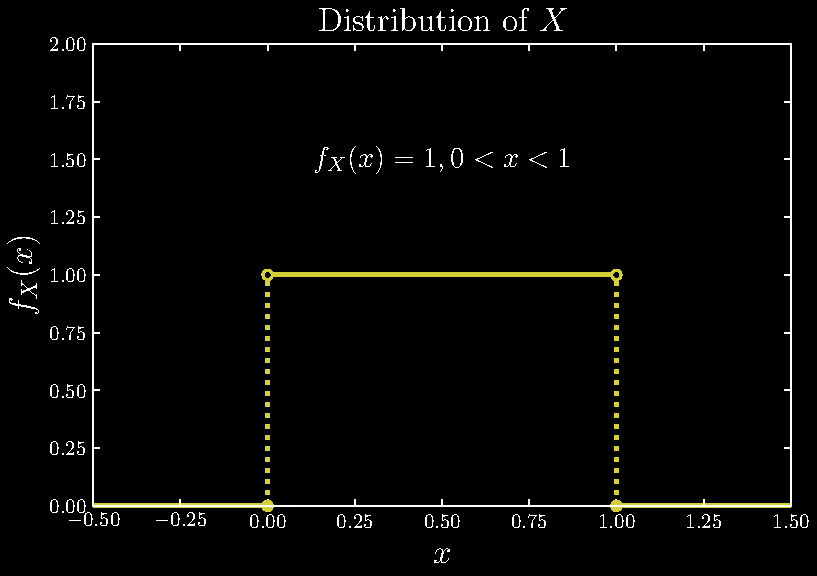
\includegraphics[width=1.0\textwidth]{chap3/chap3ex19i.eps}
\end{center}

Using the definition for \(\overline{X}_{n}\), the theoretical derivations of the expectation and variance are
\begin{align*}
	\E(\overline{X}_{n}) & = \frac{1}{n} \sum_{i=1}^{n} \E(X_{i}) \\
	 & = \frac{1}{n} \sum_{i=1}^{n} \int^{1}_{0} x_{i} \ dx_{i}  \\ 
	 & = \frac{1}{n} \sum_{i=1}^{n} \frac{1}{2} \\
	 & = \boxed{\frac{1}{2}} 
\end{align*}
Now, \(\overline{X}_{n}^{2}\) is given by
\begin{align*}
	\overline{X}_{n}^{2} & = \frac{1}{n^{2}} \left( \sum_{i=1}^{n} X_{i} \right)^{2} \\
			     & \frac{1}{n^{2}} \left( \underbrace{\sum_{i=1}^{n} X_{i}^{2}}_{n \text{ terms}} + \underbrace{\sum_{i=1}^{n} \sum_{\substack{j \neq i \\ j = 1} }^{n} X_{i} X_{j}}_{n(n-1) \text{ terms}} \right)  \\ 
\end{align*}
Using the fact that the random variables are \textsf{IID}, we can derive
\begin{align*}
	\E(\overline{X}_{n}^{2}) & = \frac{1}{n^{2}} \left( \sum_{i=1}^{n} \int^{1}_{0} x_{i}^{2} \ dx_{i} + \sum_{i=1}^{n} \sum_{\substack{j \neq i \\ j = 1}}^{n} \int^{1}_{0} x_{i} \ dx_{i} \int^{1}_{0} x_{j} \ dx_{j}    \right)  \\
	 & = \frac{1}{n^{2}} \left( n \left( \frac{1}{3} \right) + n(n-1) \left( \frac{1}{2} \right) \left( \frac{1}{2} \right)  \right)  \\ 
	 & = \frac{1}{n^{2}} \left( \frac{1}{4} n^{2} - \frac{1}{4}n + \frac{1}{3}n \right) \\
	 & = \frac{1}{4} + \frac{1}{12n} \\
	\var(\overline{X}_{n}) & = \E(\overline{X}_{n}^{2}) - \E(\overline{X}_{n})^{2} \\
	 & = \frac{1}{12n} + \frac{1}{4} - \left( \frac{1}{2} \right)^{2} \\
	 & = \boxed{\frac{1}{12n}}
\end{align*}

Empirically, we can verify that randomly generating a sampling distribution of values of \(\overline{X}_{n}\) and taking the expectation and variance agrees with the theory:

\begin{center}
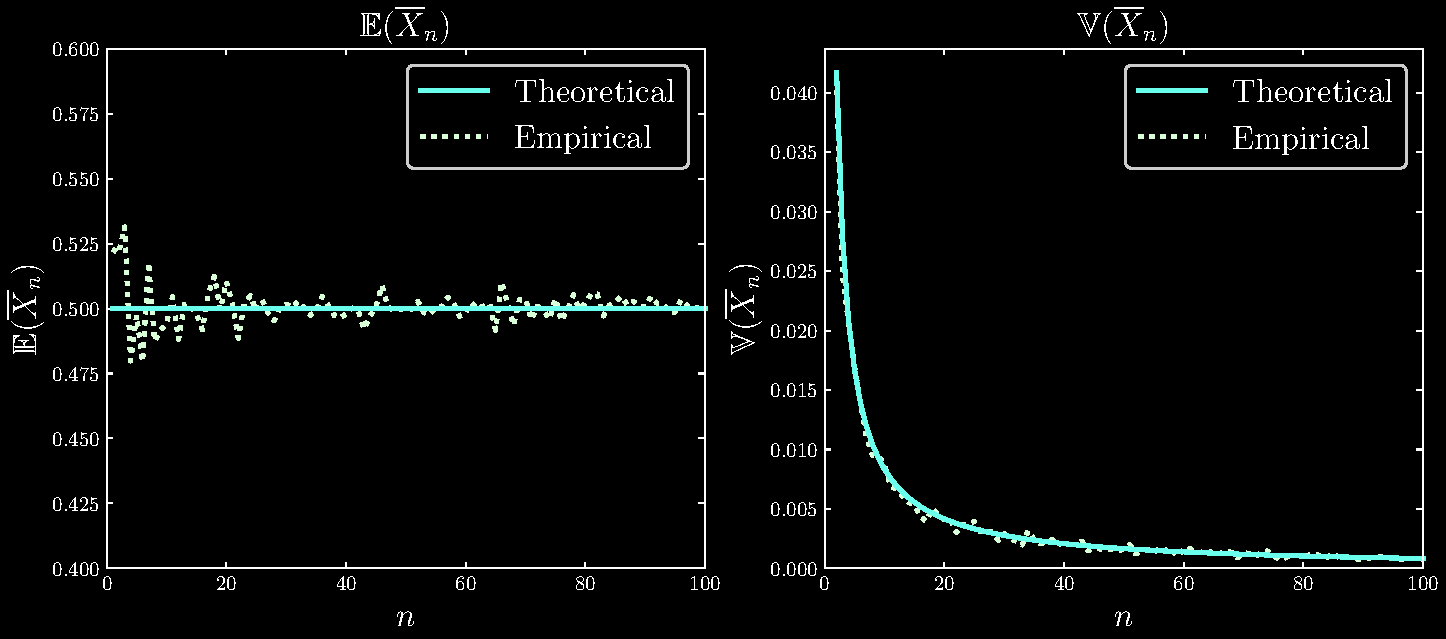
\includegraphics[width=1.0\textwidth]{chap3/chap3ex19ii.eps}
\end{center}

Lastly, we graph the sampling distributions as \(n\) increases:

\begin{center}
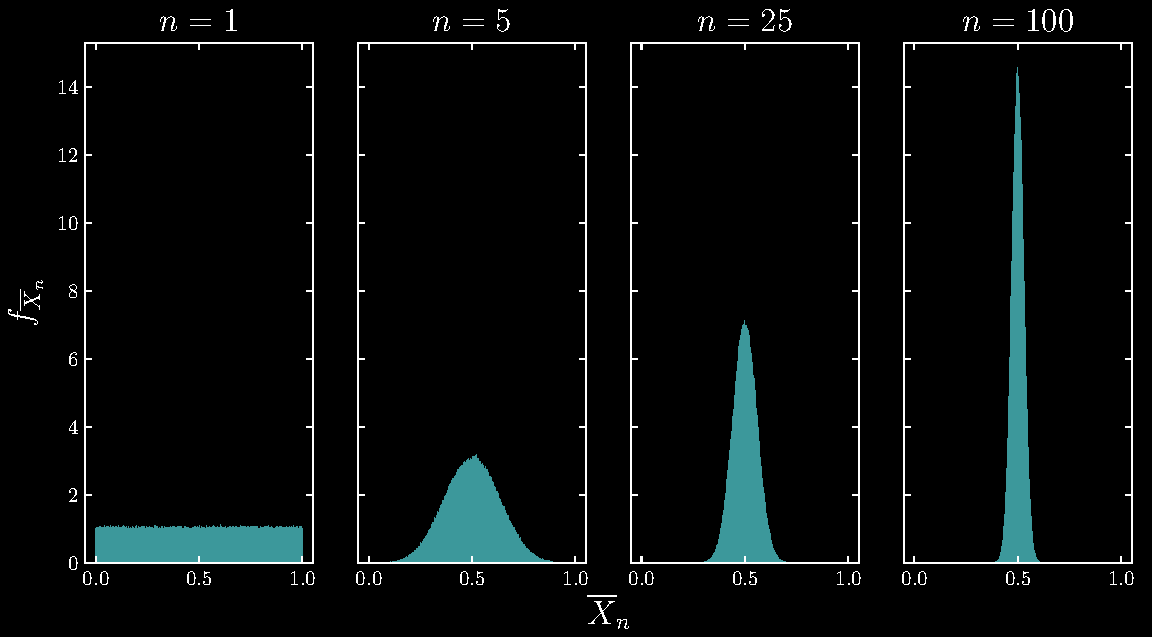
\includegraphics[width=1.0\textwidth]{chap3/chap3ex19iii.eps}
\end{center}

which gradually increases in concentration (\(\var\left( \overline{X}_{n} \right)\) goes to \(0\)) around the mean \(\E\left( \overline{X}_{n} \right) = 1/2\).

% QUESTION 20
\qs{3.8.20}{Prove Lemma 3.21.}
\lemma{(Wasserman 3.21)}{If \(a\) is a vector and \(X\) is a random vector with mean \(\mu \) and variance \(\Sigma\), then \(\E(a^{T} X) = a^{T} \mu\) and \(\var(a^{T}X) = a^{T} \Sigma a\). If \(A\) is a matrix then \(\E(AX) = A \mu \) and \(\var(AX) = A \Sigma A^{T}\). }
\begin{proof}[Proof] 
Let \(a, X \in M_{n \times 1}\), where \(M_{n \times 1}\) is the set of \(n \times 1\) vectors, and \(X\) is a random vector with mean \(\mu \) and variance \(\Sigma\).

By vector multiplication and the definition of a random vector mean, we first derive
\[
	\E(a^{T}X) = \E \left( \sum_{i=1}^{n} a_{i} X_{i} \right)  = \sum_{i=1}^{n} \E(X_{i}) = \sum_{i=1}^{n} a_{i} \mu_{i} = a^{T}\mu 
\]
Now using the definition of the variance-covariance matrix \(\Sigma\), we have \(\var(a^{T}X)\) equal to
\begin{align*}
	 & = \var \left( \sum_{i=1}^{n} a_{i} X_{i} \right)  \\
	 & = \sum_{i=1}^{n} a_{i}^{2} \var(X_{i}) + 2 \sum_{i=1}^{n} \sum_{i < j}^{n} a_{i} a_{j} \cov(X_{i}, X_{j}) \\ 
	 & = \begin{bmatrix}
		a_{1} & \cdots & a_{n} \\
	\end{bmatrix}
	 \begin{bmatrix}
		\var(X_{1}) & \cov(X_{1}, X_{2}) & \cdots & \cov(X_{1}, X_{n})  \\
		\cov(X_{2}, X_{1}) & \var(X_{2}) & \cdots & \cov(X_{2}, X_{n}) \\
		\vdots  & \vdots & \vdots & \vdots \\
		 \cov(X_{n}, X_{1}) & \cov(X_{n}, X_{2}) & \cdots & \var(X_{n}) \\
	\end{bmatrix}
	\begin{bmatrix}
		a_{1} \\
		\vdots \\
		a_{n} \\
	\end{bmatrix} \\
	 & = a^{T} \Sigma a
\end{align*}
Now let \(A \in M_{n \times n}\). Then
\[
	AX = 
	\begin{bmatrix}
		a_{11} & \cdots  & a_{1n} \\
		a_{21} & \cdots  & a_{2n} \\
		\vdots & \ddots & \vdots \\
		a_{n1} & \cdots & a_{nn}
	\end{bmatrix}
	\begin{bmatrix}
	        X_{1} \\
		X_{2} \\
		\vdots \\
		X_{n} \\
	\end{bmatrix}
	=
	\begin{bmatrix}
		\sum_{i=1}^{n} a_{1i} X_{i} \\
		\vdots \\
		\sum_{i=1}^{n} a_{ni} X_{i} \\
	\end{bmatrix}
\]
which has expectation
\begin{align*}
	\E(AX) & =
	\E\begin{bmatrix}
		\sum_{i=1}^{n} a_{1i} X_{i} \\
		\vdots \\
		\sum_{i=1}^{n} a_{ni} X_{i} \\
	\end{bmatrix} \\
	       & =
	\begin{bmatrix}
		\sum_{i=1}^{n} a_{1i} \E(X_{i}) \\
		\vdots \\
		\sum_{i=1}^{n} a_{ni} \E(X_{i}) \\
	\end{bmatrix} \\
	       & =
	\begin{bmatrix}
		\sum_{i=1}^{n} a_{1i} \mu_{i} \\
		\vdots \\
		\sum_{i=1}^{n} a_{ni} \mu_{i} \\
	\end{bmatrix} \\
	       & =
	\begin{bmatrix}
		a_{11} & \cdots  & a_{1n} \\
		a_{21} & \cdots  & a_{2n} \\
		\vdots & \ddots & \vdots \\
		a_{n1} & \cdots & a_{nn} \\
	\end{bmatrix}
	\begin{bmatrix}
		\mu_{1} \\
		\mu_{2} \\
		\vdots \\
		\mu_{n} \\
	\end{bmatrix} \\
	 & = A \mu \\ 
\end{align*}
and variance \(\var(AX)\) equal to
\[
	\begingroup
	\setlength\arraycolsep{2pt}
	\begin{bmatrix}
		\var ( \sum a_{1i} X_{i} )  & \cov(\sum a_{1i} X_{i}) &\cdots & \cov(\sum a_{1i} X_{i}, \sum a_{ni} X_{i})  \\
		\cov(\sum a_{2i} X_{i}, \sum a_{1i} X_{i}) & \var(\sum a_{2i} X_{i}) & \cdots & \cov(\sum a_{2i} X_{i}, \sum a_{ni} X_{i}) \\
		\vdots & \vdots & \vdots & \vdots \\
		\cov(\sum a_{ni} X_{i}, \sum a_{1i} X_{i}) & \cov(\sum a_{ni} X_{i}, \sum a_{2i} X_{i}) & \cdots & \var(\sum a_{ni} X_{i}) \\
	\end{bmatrix}
	\endgroup
\]
To further simplify, use the result of exercise 14 to get
\[
	\begin{bmatrix}
		\substack{\sum\limits_{i=1}^{n} a_{1i}^{2} \var(X_{i}) \\ + 2 \sum\limits_{i=1}^{n-1} \sum\limits_{i < j}^{n} a_{1i} a_{1j} \cov(X_{i}, X_{j})} & \cdots  & \sum\limits_{i=1}^{n} \sum\limits_{j=1}^{n} a_{1i} a_{1j} \cov(X_{i}, X_{j}) \\
		\sum\limits_{i=1}^{n} \sum\limits_{j=1}^{n} a_{2i} a_{1j} \cov(X_{i}, X_{j}) & \cdots  & \sum\limits_{i=1}^{n} \sum\limits_{j=1}^{n} a_{2i} a_{nj} \cov(X_{i}, X_{j}) \\
		\vdots & \ddots & \vdots \\
		\sum\limits_{i=1}^{n} \sum\limits_{j=1}^{n} a_{ni} a_{1j} \cov(X_{i}, X_{j}) & \cdots & \substack{\sum\limits_{i=1}^{n} a_{ni}^{2} \var(X_{i}) \\ + 2 \sum\limits_{i=1}^{n-1} \sum\limits_{i < j}^{n} a_{ni} a_{nj} \cov(X_{i}, X_{j})}
	\end{bmatrix}
\]
for which each entry is precisely the value of each entry in the matrix product
\[
	\begingroup
	\setlength\arraycolsep{1.55pt}
	\begin{bmatrix}
		a_{11} & \cdots  & a_{1n} \\
		a_{21} & \cdots  & a_{2n} \\
		\vdots & \ddots & \vdots \\
		a_{n1} & \cdots  & a_{nn} \\
	\end{bmatrix}
	\begin{bmatrix}
		\var(X_{1}) & \cov(X_{1}, X_{2}) & \cdots  & \cov(X_{1}, X_{n}) \\
		\cov(X_{2}, X_{1}) & \var(X_{2}) & \cdots & \cov(X_{2}, X_{n}) \\
		\vdots & \vdots & \vdots & \vdots \\
		\cov(X_{n}, X_{1}) & \cov(X_{n},X_{2}) & \cdots  & \var(X_{n}) \\
	\end{bmatrix}
	\begin{bmatrix}
		a_{11} & a_{21} & \cdots  & a_{n1} \\
		\vdots & \vdots & \ddots & \vdots \\
		a_{1n} & a_{2n} & \cdots  & a_{nn} \\
	\end{bmatrix}
	\endgroup
\]
which is \(\var(AX) = A \Sigma A^{T}\), as desired.
\end{proof}

% QUESTION 21
\qs{3.8.21}{Let \(X\) and \(Y\) be random variables. Suppose that \(\E(Y \mid X) = X\). Show that \(\cov(X,Y) = \var(X)\).}
\begin{proof}[Proof] 
Let \(\E(Y  \mid  X) = X\). Then \(\E(\E(Y  \mid  X)) = \E(Y) = \E(X)\). Moreover,
\[
	x = \int y f_{Y \mid X}(y \mid x) \ dy = \int y \frac{f_{Y,X}(y,x)}{f_{X}(x)} \ dy
\]
This implies
\begin{alignat*}{3}
	&\implies & x^{2} f_{X}(x) & = \int xy f_{Y,X}(y,x) \ dy \\
	&\implies & \int x^{2} f_{X}(x) \ dx & = \int \int xy f_{Y,X}(y,x) \ dy \ dx \\ 
	&\implies & \E(X^{2}) & = \E(XY) \\
	&\implies & \cov(X,Y) & = \E(XY) - \E(X) \E(Y) \\
	& & & = \E(X^{2}) - \E(X)^{2} \\
	& & & = \var(X)
\end{alignat*}
\end{proof}

% QUESTION 22
\qs{3.8.22}{Let \(X \sim \Uniform(0,1)\). Let \(0 < a < b < 1\). Let
\[
	Y = \begin{cases}
		1 & 0 < x < b \\
		0 & \text{otherwise} \\
	\end{cases}
\]
and let
\[
	Z = \begin{cases}
		1 & a < x < 1 \\
		0 & \text{otherwise} \\
	\end{cases}
\]
\begin{enumerate}[label=(\alph*)]
	\item Are \(Y\) and \(Z\) independent? Why/Why not?
	\item Find \(\E(Y \mid Z)\). Hint: What values \(z\) can \(Z\) take? Now find \(\E(Y  \mid  Z = z)\).
\end{enumerate}}

(a) The probabilities for all values of \(Y,Z\) are
\begin{align*}
	\Prob(Y=1) & = \int^{b}_{0}  \ dx  = b \\
	\Prob(Y=0) & = \int^{1}_{b}  \ dx = 1-b  \\ 
	\Prob(Z=1) & = \int^{1}_{a}  \ dx = 1-a \\
	\Prob(Z=0) & = \int^{a}_{0}  \ dx = a 
\end{align*}
Now, consider the following case
\[
	\Prob(Y=1,Z=1) = \int^{b}_{a}  \ dx = b-a 
\]
However,
\[
	\Prob(Y=1)\Prob(Z=1) = b(1-a) != b-a = \Prob(Y=1,Z=1)
\]
Thus \(Y\) and \(Z\) are not independent.

\par (b) The conditional expectations are
\[
	\E(Y  \mid  Z) = \begin{cases}
		\begin{aligned}
		& 1 \cdot \Prob(Y  \mid  Z=0) = \frac{\int^{a}_{0}  \ dx }{\int^{a}_{0}  \ dx } = 1 & \quad z = 0 \\
		& 1 \cdot \Prob(Y  \mid  Z=1) = \frac{\int^{b}_{a}  \ dx }{\int^{1}_{a}  \ dx } = \frac{b-a}{1-a} & \quad z = 1 \\
	\end{aligned}
	\end{cases}
\]
\newpage
% QUESTION 23
\qs{3.8.23}{Find the moment generating function for the Poisson, Normal, and Gamma distributions.}
\underline{Poisson}

For \(X \sim \Poisson(\lambda )\), we have mass
\[
	f_{X}(x) = e^{-\lambda } \frac{\lambda^{x}}{x!}
\]
with moment generating function
\begin{align*}
	\psi_{X}(t) & = \sum_{x-0}^{\infty} e^{tx} e^{-\lambda } \frac{\lambda^{x}}{x!} \\
	 & = e^{-\lambda } \sum_{x=0}^{\infty} \frac{(\lambda e^{t})^{x}}{x!} \\ 
	 & = e^{-\lambda } e^{\lambda e^{t}} \\
	 & = \boxed{e^{\lambda (e^{t} - 1)}}
\end{align*}

\underline{Normal}

For \(X \sim N(0,1)\), we have density
\[
	f_{X}(x) = \frac{1}{\sigma \sqrt{2 \pi }} \exp \left( -\frac{1}{2 \sigma^{2}} (x-\mu)^{2} \right) 
\]
with moment generating function
\begin{align*}
	\psi_{X}(t) = \E(e^{tx}) & = \frac{1}{\sigma \sqrt{2 \pi }} \int \exp \left( -\frac{1}{2 \sigma^{2}}(x-\mu)^{2} + tx \right) \ dx \\
	 & = \frac{1}{\sigma \sqrt{2 \pi }} \int \exp \left( -\frac{1}{2 \sigma^{2}} (x^{2} - 2 \mu x + \mu^{2}) + tx \right) \ dx \\ 
	 & = \frac{1}{\sigma \sqrt{2 \pi }} \int \exp \left( -\frac{1}{2 \sigma^{2}} x^{2} + \left( \frac{\mu }{\sigma^{2}} + t \right)x - \frac{\mu^{2}}{2 \sigma^{2}} \right) \ dx \\
	 & = \frac{1}{\sigma \sqrt{2 \pi }} \exp \left( -\frac{\mu^{2}}{2 \sigma^{2}} \right) \int \exp \left( -\frac{1}{2 \sigma^{2}}x^{2} + \left( \frac{\mu }{\sigma^{2}} + t \right) x \right)   \ dx 
\end{align*}
Here we complete the square by adding and subtracting \((\sigma^{2}/2)(\mu/\sigma^{2} + t)^{2}\), and writing
\[
	= \frac{1}{\sigma \sqrt{2 \pi }} \int \exp \left( -\frac{\mu^{2}}{2 \sigma^{2}} ( x - (\mu + \sigma^{2} t))^{2} + \frac{\sigma^{2}}{2} \left( \frac{\mu }{\sigma^{2}} + t \right)^{2} \right) \ dx
\]
Now substitute \(u = x - (\mu + \sigma^{2}t)\). Then \(du = dx\), and
\begin{align*}
	 & = \frac{1}{\sigma \sqrt{2 \pi }} \exp \left( -\frac{\mu^{2}}{2 \sigma^{2}} + \frac{\sigma^{2}}{2} \left( \frac{\mu }{\sigma^{2}} + t \right)^{2} \right) \int \exp \left( -\frac{1}{2 \sigma^{2}} \mu^{2} \right) \ du \\
	 & = \exp \left( -\frac{\mu^{2}}{2 \sigma^{2}} + \frac{\sigma^{2}}{2} \left( \frac{\mu }{\sigma^{2}} + t \right)^{2} \right)  \\ 
	 & = \exp \left( -\frac{\mu^{2}}{2 \sigma^{2}} + \frac{\sigma^{2}}{2} \left( \frac{\mu^{2}}{\sigma^{4}} + \frac{2 \mu }{\sigma^{2}} t + t^{2} \right)  \right) \\
	 &= \boxed{\exp \left( \mu t + \frac{1}{2} \sigma^{2} t^{2} \right) }
\end{align*}

\underline{Gamma }

For \(X \sim \gammaD(\alpha ,\beta )\), we have density
\[
	f_{X}(x) = \frac{1}{\beta^{\alpha } \Gamma(\alpha )} x^{\alpha -1} e^{-x/\beta }, \quad x, \alpha, \beta > 0
\]
where
\[
	\Gamma(\alpha ) = \int^{\infty}_{0} y^{\alpha -1} e^{-y} \ dy 
\]
and with moment generating function
\[
	\psi_{X}(t) = \E(e^{tx}) = \frac{1}{\beta^{\alpha } \Gamma(\alpha )} \int^{\infty}_{0} x^{\alpha -1} e^{-x(1/\beta - t)} \ dx 
\]
Let \(y = x (1/\beta -t)\). Then \(dy = (1/\beta -t)dx\), and we have for \(t < 1/\beta \)
\begin{align*}
	 & = \frac{1}{\beta^{\alpha } \Gamma(\alpha )} \frac{1}{(1/\beta - t)^{\alpha }} \int^{\infty}_{0} y^{\alpha -1} e^{-y} \ dy  \\
	 & = \frac{1}{\beta^{\alpha } \Gamma(\alpha )} \frac{1}{(1/\beta^{\alpha }) (1-t \beta )^{\alpha }}\Gamma(\alpha ) \\ 
	 & = \boxed{(1 - t \beta )^{-\alpha }}
\end{align*}

% QUESTION 24
\qs{3.8.24}{Let \(X_{1}, dots, X_{n} \sim \Exp(\beta )\). Find the moment generating function of \(X_{i}\). Prove that \(\sum_{i=1}^{n} X_{i} \sim \gammaD(n, \beta )\).}
\begin{proof}[Proof] 
For \(X_{i} \sim \Exp(\beta )\), we have density
\[
	f_{X_{i}}(x_{i}) = \frac{1}{\beta } \exp(-x_{i}/\beta ), \quad x_{i}, \beta >0
\]
with moment generating function
\begin{align*}
	\psi_{X_{i}}(t) = \E(e^{tx}) & = \frac{1}{\beta } \int^{\infty}_{0} \exp(-x(1/\beta -t) \ dx  \\
	 & = \frac{1}{1-t \beta } 
\end{align*}
for \( t < 1/\beta \). By Lemma 3.31(2) and assuming independence of the \(X_{i}\)'s, for \(X = \sum_{i=1}^{n} X_{i}\) we have
\[
	\psi_{X}(t) = \prod_{i} \psi_{X_{i}}(t) = \prod_{i} (1 - t \beta ) = (1-t \beta )^{-n}   
\]
Implying \(X \sim \gammaD(n, \beta )\) per the results of exercise 3.8.23.

\end{proof}

\section{Chapter 4: Inequalities}

\subsection*{Import Packages}

Please see the associated GitHub repo for all code and comments to simulations. [LINK HERE]

\begin{python}
import numpy as np
from numpy.random import choice
import random
import matplotlib.pyplot as plt
import scienceplots
\end{python}

% QUESTION 1
\qs{4.5.1}{Let \(X \sim \Exp\left( \beta  \right)\). Find \(\Prob\left(\abs{X - \mu_{X}} \ge k \sigma_{X}\right)\) for \(k > 1\). Compare this to the bound you get from Chebyshev's inequality.}

For \(X \sim \Exp\left( \beta  \right)\), \(\mu_{X} = \beta \) and \(\sigma_{X}^{2} = \beta^{2}\). Calculating the probability exactly,
\begin{align*}
	\Prob\left( \abs{X - \mu_{X}} \ge k \sigma_{X} \right) & = \Prob\left( X - \mu_{X} \ge k \beta \right)  \\
	 & = \Prob\left( X \ge (k+1)\beta \right)  \\ 
	 & = \frac{1}{\beta} \int^{\infty}_{(k+1)\beta } \exp\left( -x/\beta  \right)  \ dx \\
	 & = -\exp\left( -x/\beta  \right) \bigg|^{\infty}_{(k+1)\beta } \\
	 & = \exp\left( -(k+1) \right)
\end{align*}
with the first equality following from the fact that since \(x > 0\), \(\mu = \sigma_{X} = \beta \), no \(x\) can be \(k \sigma_{X} = k \beta \) to the left of the mean.


By Chebyshev's inequality,
\[
	\Prob\left( \abs{X - \beta } \ge k \sigma_{X} \right) \le \frac{\sigma_{X}^{2}}{k^{2} \sigma_{X}^{2}} = \frac{1}{k^{2}}
\]
where \(\exp\left( -(k+1) \right) < 1/k^{2}\) for \(k > 1\).

Here we graph the exact probability and the Chebyshev bound as functions of \(k\):

\begin{center}
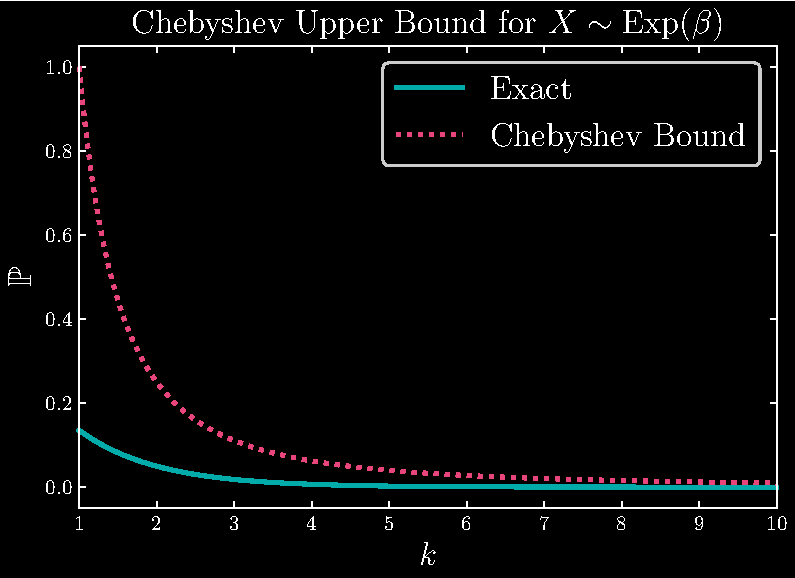
\includegraphics[width=1.0\textwidth]{chap4/chap4ex1.eps}
\end{center}

% QUESTION 2
\qs{4.5.2}{Let \(X \sim \Poisson\left( \lambda  \right)\). Use Chebyshev's inequality to show that \(\Prob\left( X \ge 2 \lambda  \right) \le 1/\lambda \).}
\begin{proof}[Proof] 
For \(X \sim \Poisson\left( \lambda  \right)\), we have \(\mu_{X} = \sigma_{X}^{2} = \lambda \). In the case where \(X - \lambda \ge 0\) and \(t = \lambda \), we have
\begin{align*}
	\Prob\left( \abs{X - \lambda} \ge \lambda \right) & = \Prob\left( X - \lambda \ge \lambda  \right) \\
	 & = \Prob\left( X \ge 2 \lambda  \right) \\ 
\end{align*}
Note that when \(X - \lambda < 0\) with \(t = \lambda \), we have
\begin{align*}
	\Prob\left( \abs{X - \lambda} \ge t \right) & = \Prob\left( -\left( X - \lambda  \right) \ge \lambda  \right)  \\
	 & = \Prob\left( X \le \lambda - \lambda  \right) \\
	 & = \Prob\left( X \le 0 \right) \\
	 & = 0
\end{align*}
so we need only consider the case where \(X - \lambda \ge 0\). Applying Chebyshev's inequality, we can conclude
\[
	\Prob\left( X \ge 2 \lambda  \right) \le \frac{\lambda }{\lambda^{2}} = \frac{1}{\lambda }
\]
\end{proof}

% QUESTION 3
\qs{4.5.3}{Let \(X_{1}, \dots, X_{n} \sim \Bernoulli\left( p \right)\) and \(\overline{X}_{n} = n^{-1} \sum_{i=1}^{n} X_{i}\). Bound \(\Prob\left( \abs{\overline{X}_{n} - p} > \epsilon \right)\) using Chebyshev's inequality and using Hoeffding's inequality. Show that, when \(n\) is large, the bound from Hoeffding's inequality is smaller than the bound from Chebyshev's inequality.}
\begin{proof}[Proof] 
For \(\overline{X}_{n}\), we have \(\E\left( \overline{X}_{n} \right) = p\) and \(\var\left( \overline{X}_{n} \right) = p \left( 1-p \right) / n\). The upper bounds from Chebyshev and Hoeffding are
\begin{align*}
	\Prob\left( \abs{\overline{X}_{n} - p} > \epsilon  \right) & \le \frac{p \left( 1-p \right) }{n \epsilon^{2}} &&\text{(Chebyshev)} \\
	\Prob\left( \abs{\overline{X}_{n} - p} > \epsilon  \right) & \le 2 e^{-2n \epsilon^{2}}  &&\text{(Hoeffding)} \\ 
\end{align*}
Taking the ratio of the Hoeffding to Chebyshev limits, we aim to calculate
\[
	\lim_{n \to \infty} \frac{2 e^{-2n \epsilon^{2}}}{p(1-p) / n \epsilon^{2}} = \frac{1}{p \left( 1-p \right) }\lim_{n \to \infty} \frac{2n \epsilon^{2}}{e^{2n \epsilon^{2}}}
\]
Using l'H\^{o}pital's rule to evaluate the limit since \(\lim_{n \to \infty} 2n \epsilon^{2} = +\infty\) and \(\lim_{n \to \infty} e^{2n \epsilon^{2}} = +\infty\), we have
\[
\frac{1}{p \left( 1-p \right) } \lim_{n \to \infty} \frac{2n \epsilon^{2}}{e^{2n \epsilon^{2}}} = \frac{1}{p \left( 1-p \right)} \lim_{n \to \infty} \frac{2 \epsilon^{2}}{2 \epsilon^{2} e^{2n \epsilon^{2}}} = \frac{1}{p \left( 1-p \right)} \lim_{n \to \infty} \frac{1}{e^{2n \epsilon^{2}}} = 0
\]
ascertaining that Hoeffding is a tighter bound than Chebyshev.
\end{proof}

\newpage
% QUESTION 4
\qs{4.5.4}{Let \(X_{1}, \dots, X_{n} \sim \Bernoulli\left( p \right)\).
\begin{enumerate}[label=(\alph*)]
	\item Let \(\alpha > 0\) be fixed and define
		\[
			\epsilon_{n} = \sqrt{\frac{1}{2n} \log\left( \frac{2}{\alpha } \right)}.
		\]
	Let \(\widehat{p}_{n} = n^{-1} \sum_{i=1}^{n} X_{i}\). Define \(C_{n} = \left(\widehat{p}_{n} - \epsilon_{n}, \widehat{p}_{n} + \epsilon_{n}\right)\). Use Hoeffding's inequality to show that
	\[
		\Prob\left( C_{n} \text{ contains } p \right) \ge 1 - \alpha .
	\]
	In practice, we truncate the interval so it does not go below 0 or above 1.
	\item \textsf{(Computer Experiment.)} Let's examine the properties of this confidence interval. Let \(\alpha = 0.05\) and \(p = 0.4\). Conduct a simulation study to see how often the interval contains \(p\) (called the coverage). Do this for various values of \(n\) between 1 and 10000. Plot the coverage versus \(n\).
	\item Plot the length of the interval versus \(n\). Suppose we want the length of the interval to be no more than \(.05\). How large should \(n\) be?
\end{enumerate}}
\begin{proof}[Proof] 
	(a) Since \(\overline{X}_{n} = \widehat{p}_{n}\) and \(\Prob\left( \abs{\overline{X}_{n} - p} > \epsilon_{n} \right) \le \alpha \), by complementary events (either \(\abs{\overline{X}_{n} - p} > \epsilon_{n}\) or \(\abs{\overline{X}_{n} - p} \le \epsilon_{n}\)), we have
\[
	\Prob\left( \abs{\overline{X}_{n} - p} \le \epsilon_{n} \right) \ge 1 - \alpha 
\]
\end{proof}

\par (b) Here, we sample numerous values of \(\widehat{p}_{n}\), construct \(C_{n}\) from each value, and determine if \(p \in C_{n}\). 

\begin{python}
k, n = 1000, 10000
alpha = 0.05
eps = np.sqrt((1/(2*n))*np.log(2/alpha))
p = 0.4

def confinttest(k,n):
    s = np.random.binomial(1,p,size=(k,n)).mean(axis=1)
    return (p > s - eps) & (p < s + eps);

def coverage():
    coverage = []
    for i in range(1,n+1):
        count = np.count_nonzero(confinttest(k,i) == True)
        coverage.append(count / k)
    return coverage;
\end{python}

\begin{center}
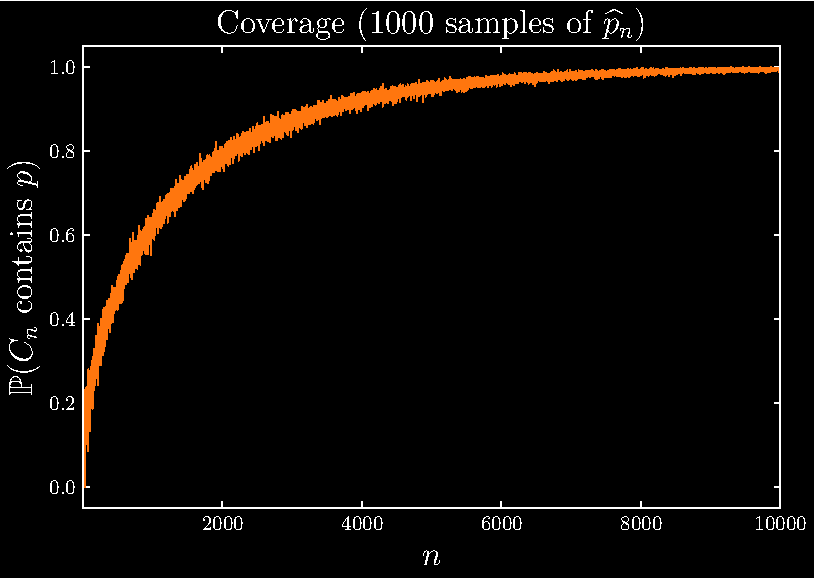
\includegraphics[width=1.0\textwidth]{chap4/chap4ex4b}
\end{center}

As \(n \rightarrow +\infty\), we see that the coverage asymptotically approaches 1. Intuitively this is sensible. Since \(X_{i} \sim \Bernoulli\left( p \right)\), for large \(n\), \(\widehat{p}_{n} \rightarrow p\) (this is the weak law of large numbers, covered in the next chapter). 

\par (c) The length of \(C_{n}\) is \(2 \epsilon_{n}\), and for the length to be no more than \(0.05\), have \(n \ge 2952\).

\begin{python}
def intlength(n):
    epsilons = np.empty(n)
    for i in range(1,n+1):
        epsilon = np.sqrt((1/(2*i))*np.log(2/alpha))
        epsilons[i-1] = 2*epsilon
    return epsilons;

n = 5000
nsolution = np.argwhere(intlength(n) < 0.05).min() + 1
\end{python}

\begin{center}
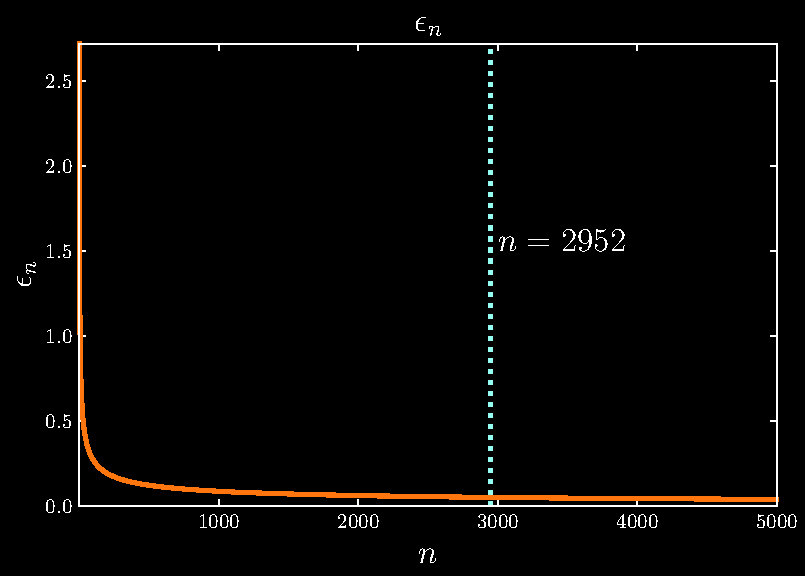
\includegraphics[width=1.0\textwidth]{chap4/chap4ex4c.eps}
\end{center}


% QUESTION 5
\qs{4.5.5}{Prove Mill's inequality, Theorem 4.7. Hint. Note that \(\Prob\left( \abs{Z} > t \right) = 2 \Prob\left( Z > t \right)\). Now write out what \(\Prob\left( Z > t \right)\) means and note that \(x/t > 1\) whenever \(x > t\).}
\thm{(Wasserman 4.7) (Mill's Inequality)}{Let \(Z \sim N \left( 0,1 \right) \). Then
\[
	\Prob\left( \abs{Z} > t \right) \le \sqrt{\frac{2}{\pi }} \frac{e^{-t^{2}/2}}{t}.
\]}
\begin{proof}[Proof] 
By symmetry of the standard normal distribution, 
\[
	\Prob\left( \abs{Z} > t \right) = 2 \Prob\left( Z > t \right)
\] 
Then
\begin{align*}
	\Prob\left( \abs{Z} > t \right) & = 2 \Prob\left( Z > t \right) \\
	 & = 2 \int^{\infty}_{t} \frac{1}{\sqrt{2 \pi }} \exp\left( -\frac{z^{2}}{2} \right) \ dz \\ 
\end{align*}
Now, multiply both sides by \(t\):
\begin{align*}
	\implies t \Prob\left( \abs{Z} > t \right) & = \sqrt{\frac{2}{\pi }} t \int^{\infty}_{t} \exp\left( -\frac{z^{2}}{2} \right) \ dz  \\
	 & \le \sqrt{\frac{2}{\pi }} \int^{\infty}_{t} z \exp\left( -\frac{z^{2}}{2} \right) \ dz  \\ 
	 & = \sqrt{\frac{2}{\pi }} e^{-t^{2}/2}
\end{align*}
which lastly implies that \(\Prob\left( \abs{Z} > t \right) \le \sqrt{\frac{2}{\pi }} e^{-t^{2}/2} / t\).
\end{proof}

% QUESTION 6
\qs{4.5.6}{Let \(Z \sim N \left( 0,1 \right) \). Find \(\Prob\left( \abs{Z} > t \right)\) and plot this as a function of \(t\). From Markov's inequality, we have the bound \(\Prob\left( \abs{Z} > t \right) \le \frac{\E\left| Z \right|^{k}}{t^{k}}\) for any \(k>0\). Plot these bounds for \(k = 1,2,3,4,5\) and compare them to the true value of \(\Prob\left( \abs{Z} > t \right)\). Also, plot the bound from Mill's inequality.}

Some initial observations to bear in mind:
\begin{itemize}
	\item Observe that \(\Prob\left( \abs{Z} > t \right)\) is the two-tailed probability that we observe \(Z > t\), when \(Z \ge 0\), or \(Z < -t\), when \(Z < 0\).
	\item Using Markov's inequality, \(\Prob\left( \abs{Z} > t \right) = \Prob\left( \abs{Z}^{k} > t^{k} \right) \le \E \abs{Z}^{k} / t^{k} \). 
	\item The expectation term \(\E\left( \abs{Z} \right)\) is defined as
\[
	\E \abs{Z} = \int^{+\infty}_{0} z f_{Z}\left( z \right) \ dz + \int^{0}_{-\infty} z f_{Z}\left( z \right) \ dz = 2 \int^{+\infty}_{0} z f_{Z}\left( z \right) \ dz = \sqrt{\frac{2}{\pi }} 
\]
\end{itemize}

Running a horse race between the exact two-tail probability and the Markov and Mill bounds, we find:

\begin{python}
def normtest(t): 
    normal_dist = norm(0,1)
    domain = np.arange(0,t+0.01,0.01)
    probs = np.empty(len(domain))
    for i, j in zip(domain, range(0, len(domain))):
        probs[j] = (2*(1-normal_dist.cdf(i)))
    return probs;

def markov(k, t):
    domain = np.arange(0.01,t+0.01,0.01)
    markovs = np.empty(len(domain))
    exptabszk = np.power(
    		np.absolute(np.random.normal(0,1,1000)), k).mean()
    for i, j in zip(domain, range(0, len(domain))):
        markovs[j] = np.divide(exptabszk, np.power(i,k))
    return markovs;

def mill(t):
    domain = np.arange(0.01,t+0.01,0.01)
    mills = np.empty(len(domain))
    for i, j in zip(domain, range(0, len(domain))):
        mills[j] = np.sqrt(2 / math.pi)*(np.exp(-np.square(i)/2)/i)
    return mills;

t = 5.5
\end{python}

\begin{center}
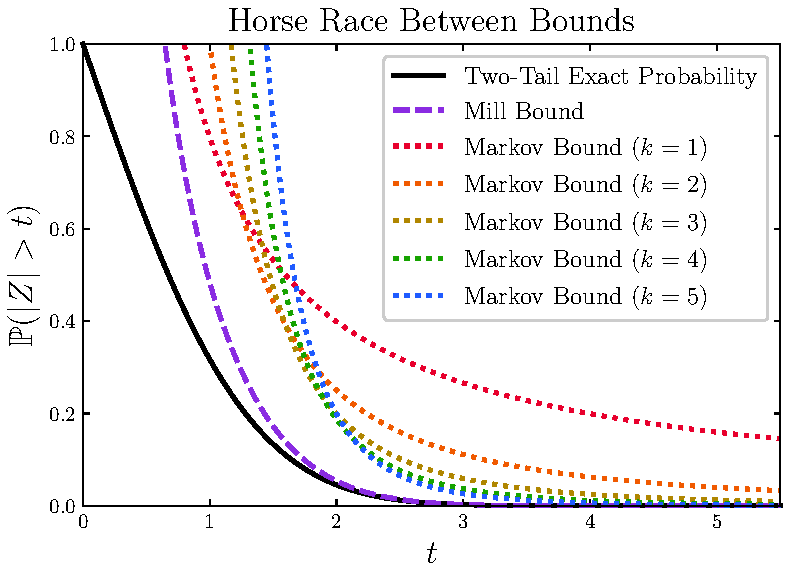
\includegraphics[width=1.0\textwidth]{chap4/chap4ex6.eps}
\end{center}

% QUESTION 7
\qs{4.5.7}{Let \(X_{1}, \dots, X_{n} \sim N \left( 0,1 \right) \). Bound \(\Prob\left( \abs{\overline{X}_{n}} > t \right)\) using Mill's inequality, where \(\overline{X}_{n} = n^{-1} \sum_{i=1}^{n} X_{i}\). Compare to the Chebyshev bound.}
First note that \(\E\left( \overline{X}_{n} \right) = 0\) and \(\var\left( \overline{X}_{n} \right) = 1/n\). Thus \(\overline{X}_{n} \sim N \left( 0, 1/n \right) \). In order for Mill's inequality to be applicable, we transform \(\overline{X}_{n}\) and \(t\) to be standard normal:
\begin{align*}
	\Prob\left( \left|\frac{\overline{X}_{n}}{\sqrt{1/n}} \right| > \frac{t}{\sqrt{1/n}}\right) & = \Prob\left( \left|\frac{\overline{X}_{n}}{\sqrt{1/n}} \right| > \sqrt{n}t \right)  \\
	 & \le \sqrt{\frac{2}{\pi }} \frac{e^{- \left( \sqrt{n}t \right)^{2} / 2}}{\sqrt{n} t} \\ 
	 & = \sqrt{\frac{2}{n \pi }} \frac{e^{-nt^{2}/2}}{t}
\end{align*}

And Chebyshev's inequality is given simply by
\[
	\Prob\left( \abs{\overline{X}_{n}} \ge t \right) \le \frac{1}{n t^{2}}
\]
Taking the limit of the ratio of the Mill bound to the Chebyshev for large \(n\) gives us
\[
	\lim_{n \to \infty} \frac{\sqrt{\frac{2}{ n \pi}} \frac{e^{-nt^{2}/2}}{t}}{1 / nt^{2}} = \lim_{n \to \infty} \sqrt{\frac{2n}{\pi }} t e^{-nt^{2}/2} = \boxed{0}
\]
yielding the conclusion that Mill is a smaller bound than Chebyshev.
	

\section{Chapter 5: Convergence of Random Variables}

% QUESTION 1
\qs{5.8.1}{Let \(X_{1}, \dots, X_{n}\) be \textsf{IID} with finite mean \(\mu = \E\left( X_{1} \right)\) and finite variance \(\sigma^{2} = \var\left( X_{1} \right)\). Let \(\overline{X}_{n}\) be the sample mean and let \(S^{2}_{n}\) be the sample variance.

\begin{enumerate}[label=(\alph*)]
	\item Show that \(\E\left( S^{2}_{n} \right) = \sigma^{2}\).
	\item Show that \(S^{2}_{n} \xrightarrow{\text{ P }} \sigma^{2}\). Hint: Show that \(S^{2}_{n} = c_{n} n^{-1} \sum_{i=1}^{n} X^{2}_{i} - d_{n} \overline{X}^{2}_{n}\) where \(c_{n} \rightarrow 1\) and \(d_{n} \rightarrow 1\). Apply the law of large numbers to \(n^{-1} \sum_{i=1}^{n} X^{2}_{i}\) and to \(\overline{X}_{n}\). Then use part (d) of Theorem 5.5.
\end{enumerate}}
\begin{proof}[Proof] 
\par (a) See exercise 3.8.8, which provides a proof of Theorem 3.17.
\vspace{12pt}
\par (b) Using the hint, we can write \(S^{2}_{n}\) as
\begin{align*}
	S^{2}_{n} & = \frac{1}{n-1} \sum_{i=1}^{n} \left( X_{i} - \overline{X}_{n} \right)^{2} \\
	 & = \frac{1}{n-1} \sum_{i=1}^{n} \left( X^{2}_{i} - 2X_{i} \overline{X}_{n} + \overline{X}^{2}_{n} \right)  \\ 
	 & = \frac{1}{n-1} \sum_{i=1}^{n} X^{2}_{i} - \frac{n}{n-1} \overline{X}^{2}_{n} \\
	 & = c_{n} \frac{1}{n} \sum_{i=1}^{n} X^{2}_{i} - d_{n} \overline{X}^{2}_{n}
\end{align*}
where \(c_{n} = d_{n} = \frac{n}{n-1} \rightarrow 1\) as \(n \rightarrow \infty\).

By WLLN, \(\overline{X}_{n} \xrightarrow{\text{ P }} \mu \). By Theorem 5.5(f), \(\overline{X}^{2}_{n} \xrightarrow{\text{ P }} \mu^{2}\). 

For the \(\frac{1}{n} \sum_{i=1}^{n} X^{2}_{n}\) term, the task is to determine if \(X^{2}_{1}, \dots, X^{2}_{n}\) are \textsf{IID}. Recall from exercise 2.14.10 that if \(X \sqcup Y\), and if \(g, h\) are functions, then \(g \left( X \right) \sqcup h \left( Y \right) \). Therefore, for \(X_{i}, X_{j}\) such that \(i \neq j\), we must have \(X^{2}_{i} \sqcup X^{2}_{j}\). Since the \(X_{i}\)'s come from identical distributions, so must the \(X^{2}_{i}\)'s.

Thus, since \(\E\left( X^{2}_{1} \right) = \sigma^{2} + \mu^{2}\), by WLLN, \(\frac{1}{n} \sum_{i=1}^{n} X^{2}_{i} \xrightarrow{\text{ P }} \sigma^{2} + \mu^{2}\). Ergo, applying Theorem 5.5(d) to the products \(c_{n} \frac{1}{n} \sum_{i=1}^{n} X^{2}_{i}\) and \(d_{n} \overline{X}^{2}_{n}\), we find
\[
	S^{2}_{n} = c_{n} \frac{1}{n} \sum_{i=1}^{n} X^{2}_{i} - d_{n} \overline{X}^{2}_{n} \xrightarrow{\text{ P }} \sigma^{2} + \mu^{2} - \mu^{2} = \sigma^{2}
\]
\end{proof}

\newpage
% QUESTION 2
\qs{5.8.2}{Let \(X_{1}, X_{2}, \dots \) be a sequence of random variables. Show that \(X_{n} \xrightarrow{\text{qm}} b\) if and only if
\[
	\lim_{n \to \infty} \E\left( X_{n} \right) = b \quad \text{and}\quad \lim_{n \to \infty} \var\left( X_{n} \right) = 0.
\]}

\begin{proof}[Proof] 
\(\left( \implies \right)\)  Let \(X_{n} \xrightarrow{\text{qm}} b\). Then \(\E\left( X_{n} - b \right)^{2} \rightarrow 0\). By Theorem 5.17(b), we also have that \(X_{n}\) converges in \(L_{1}\) to \(b\):
\[
	\E\left| X_{n} - b \right| \rightarrow 0
\]
If \(X_{n} - b \ge 0\), then \(\E\left|X_{n} - b \right| = \E\left( X_{n} - b \right)\), and 
\[
	\lim_{n \to \infty} \E\left( X_{n} - b \right) = \lim_{n \to \infty} \E\left( X_{n} \right) - b = 0 \implies \lim_{n \to \infty} \E\left( X_{n} \right) = b
\]

Otherwise, \(\E\left| X_{n} - b \right| = \E\left( -\left( X_{n} - b \right)  \right)\), and 
\[
	\lim_{n \to \infty} \E\left( - \left( X_{n} - b \right)  \right) = 0 \implies \lim_{n \to \infty} \E\left( X_{n} - b \right) \implies \lim_{n \to \infty} \E\left( X_{n} \right) = b
\] 

as before.

Thus we must have \(\lim_{n \to \infty}  \E\left( X_{n} \right) = b\) in either case. Combining this fact and the premise, it must follow that
\begin{align*}
	\lim_{n \to \infty} \E\left( X_{n} - b \right)^{2} & = \lim_{n \to \infty} \E\left( X^{2}_{n} - 2bX_{n} + b^{2} \right) \\
	& = \lim_{n \to \infty} \E\left( X^{2}_{n} \right) - 2b \lim_{n \to \infty} \E\left( X_{n} \right) + b^{2} \\
	& = \lim_{n \to \infty} \E\left( X^{2}_{n} \right) - 2 \lim_{n \to \infty} \E\left( X_{n} \right)^{2} + \lim_{n \to \infty} \E\left( X_{n} \right)^{2} \\
	& = \lim_{n \to \infty} \left[ \E\left( X^{2}_{n} \right) - \E\left( X_{n} \right)^{2} \right] \\
	& = \lim_{n \to \infty} \E\left( X_{n} - \E\left( X_{n} \right) \right)^{2} \\
	& = \lim_{n \to \infty} \var\left( X_{n} \right) \\
	& = 0
\end{align*}

\(\left( \impliedby \right) \) In the converse direction, let
\[
	\lim_{n \to \infty} \E\left( X_{n} \right) = b \qquad \lim_{n \to \infty} \var\left( X_{n} \right) = 0
\]
Then 
\begin{align*}
	\lim_{n \to \infty} \var\left( X_{n} \right) & = \lim_{n \to \infty} \E\left( X_{n} - \E\left( X_{n} \right) \right)^{2}  \\
	& = \lim_{n \to \infty} \E\left( X^{2}_{n} - 2 X_{n} \E\left( X_{n} \right) + \E\left( X_{n} \right)^{2} \right) \\
	& = \lim_{n \to \infty} \E\left( X^{2}_{n} \right) - 2 \lim_{n \to \infty} \E\left( X_{n} \right)^{2} + \lim_{n \to \infty} \E\left( X_{n} \right)^{2} \\
	& = \lim_{n \to \infty} \E\left( X^{2}_{n} \right) - b^{2} \\
	& = \lim_{n \to \infty} \E\left( X_{n} - b \right)^{2} \\
	& = 0
\end{align*}
implies \(X_{n} \xrightarrow{\text{qm}} b\).
\end{proof}

% QUESTION 3
\qs{5.8.3}{Let \(X_{1}, \dots, X_{n}\) be \textsf{IID} and let \(\mu = \E\left( X_{1} \right)\). Suppose that the variance is finite. Show that \(\overline{X}_{n} \xrightarrow{\text{qm}} \mu \).}
\begin{proof}[Proof] 
Since \(\E\left( \overline{X}_{n} \right) = \mu \) and \(\var\left( \overline{X}_{n} \right) = \sigma^{2} / n\), observe that
\begin{align*}
	\lim_{n \to \infty} \E\left( \overline{X}_{n} \right) & = \lim_{n \to \infty} \mu = \mu  \\
	\lim_{n \to \infty} \var\left( \overline{X}_{n} \right) & = \lim_{n \to \infty} \frac{\sigma^{2}}{n} = 0 \\ 
\end{align*}
By exercise 5.8.2, \(\overline{X}_{n} \xrightarrow{\text{qm}} \mu \).
\end{proof}

% QUESTION 4
\qs{5.8.4}{Let \(X_{1}, X_{2}, \dots\) be a sequence of random variables such that
\[
	\Prob\left( X_{n} = \frac{1}{n} \right) = 1 - \frac{1}{n^{2}} \quad \text{and} \quad \Prob\left( X_{n} = n \right) = \frac{1}{n^{2}}.
\]
Does \(X_{n}\) converge in probability? Does \(X_{n}\) converge in quadratic mean?}

By the errata, note that \(n \ge 2\).

\underline{Conjecture:} \(X_{n} \xrightarrow{\text{ P }} 0 \)

\begin{proof}[Proof] 
Observe that \(\lim_{n \to \infty} \Prob\left( \abs{X_{n}} > \epsilon  \right) = \Prob\left( n > \epsilon \text{ or } \frac{1}{n} > \epsilon  \right)\). Then by mutual exclusivity:
\begin{align*}
	 & = \lim_{n \to \infty} \Prob\left( n > \epsilon  \right)\Prob\left( X_{n} = n \right) + \lim_{n \to \infty} \Prob\left( \frac{1}{n} > \epsilon  \right) \Prob\left( X_{n} = \frac{1}{n} \right) \\
	 & = \lim_{n \to \infty} \Prob\left( n > \epsilon  \right) \frac{1}{n^{2}} + \lim_{n \to \infty} \Prob\left( \frac{1}{n} > \epsilon  \right) \left( 1 - \frac{1}{n^{2}} \right)  \\ 
	 & = \lim_{n \to \infty} \Prob\left( \frac{1}{n} > \epsilon  \right) \\
	 & = 0
\end{align*}
Thus \(X_{n} \xrightarrow{\text{ P }} 0\).
\end{proof}

\underline{Conjecture:} \(X_{n} \xrightarrow{\text{qm}} X\)

\begin{proof}[Proof] 
Suppose \(X_{n}\) converges in quadratic mean to \(X\). Then we have
\begin{align*}
	\E\left( X_{n} - X \right)^{2} & = \E\left( X^{2}_{n} - 2X_{n}X + X^{2} \right) \\
	 & = \E\left( X^{2}_{n} \right) - 2 \E\left( X_{n}X \right) + \E\left( X^{2} \right) \\
	 & = \frac{1}{n^{2}} \left( 1 - \frac{1}{n^{2}} \right) + n^{2} \left( \frac{1}{n^{2}} \right) \\
	 & \qquad - 2 \left( \frac{1}{n} \E\left( X \right) \left( 1 - \frac{1}{n^{2}} \right) + n \E\left( X \right) \left( \frac{1}{n^{2}} \right)  \right) + \E\left( X^{2} \right) \\
\end{align*}
Now take the limit for large \(n\) to find
\[
	\lim_{n \to \infty} \E\left( X_{n} - X \right)^{2} = 1 + \E\left( X^{2} \right)
\]
Now, by our initial assumption, we must have
\[
	1 + \E\left( X^{2} \right) = 0
\]
But this is impossible, as it would require \(\E\left( X^{2} \right) = -1\), which can never be the case since \(\var\left( X \right) \ge 0\). So \(X_{n} \centernot{\xrightarrow{\text{qm}}} X\) for any \(X\).
\end{proof}

% QUESTION 5
\qs{5.8.5}{Let \(X_{1}, \dots, X_{n} \sim \Bernoulli\left( p \right)\). Prove that
\[
	\frac{1}{n} \sum_{i=1}^{n} X^{2}_{i} \xrightarrow{\text{ P }} p \quad \text{and} \quad \frac{1}{n} \sum_{i=1}^{n} X^{2}_{i} \xrightarrow{\text{qm}} p.
\]}
\begin{proof}[Proof] 
First we prove that \(\frac{1}{n} \sum_{i=1}^{n} X^{2}_{i} \xrightarrow{\text{qm}} p\). The expectation and mean are
\begin{align*}
	\E\left( \frac{1}{n} \sum_{i=1}^{n} X^{2}_{i} \right) & = \frac{1}{n} \sum_{i=1}^{n} \E\left( X^{2}_{i} \right) \\
	 & = \frac{1}{n} np \\ 
	 & = p \\
	\var\left( \frac{1}{n} \sum_{i=1}^{n} X^{2}_{i} \right) & = \frac{1}{n^{2}} \sum_{i=1}^{n} \var\left( X^{2}_{i} \right) \\
	 & = \frac{1}{n} \left[ \E\left( X^{4}_{i} \right) - \E\left( X^{2}_{i} \right)^{2} \right] \\
	 & = \frac{1}{n} \left( p - p^{2} \right) 
\end{align*}
So we ascertain that 
\[
	\E\left( \frac{1}{n} \sum_{i=1}^{n} X^{2}_{i} - p \right)^{2} = \var\left( \frac{1}{n} \sum_{i=1}^{n} X^{2}_{i} \right)
\]
and that the remaining task is to prove the variance vanishes in the limit:
\[
	\lim_{n \to \infty} \var\left( \frac{1}{n} \sum_{i=1}^{n} X^{2}_{i} \right) = \lim_{n \to \infty} \frac{1}{n} \left( p - p^{2} \right) = 0
\]
Thus \(\frac{1}{n} \sum_{i=1}^{n} X^{2}_{i} \xrightarrow{\text{qm}} p \). By Theorem 5.4(a), it immediately follows that \(\frac{1}{n} \sum_{i=1}^{n} X^{2}_{i} \xrightarrow{\text{ P }} p\).
\end{proof}

% QUESTION 6
\qs{5.8.6}{Suppose that the height of men has mean 68 inches and standard deviation 2.6 inches. We draw 100 men at random. Find (approximately) the probability that the average height of men in our sample will be at least 72 inches.}

Note that the errata is for 72 inches.

For \(Z \sim N \left( 0,1 \right) \), by the Central Limit Theorem:

\begin{align*}
	\Prob\left( \overline{X}_{n} > 72 \right) & = \Prob\left( \frac{\sqrt{100} \left( \overline{X}_{n} - 68  \right) }{2.6} > \frac{\sqrt{100} \left( 72 - 68 \right) }{2.6} \right) \\
	 & \approx \Prob\left( 10 Z > 15.38 \right) \\ 
	 & = \Prob\left( Z > 1.538 \right) \\
	 & \approx \boxed{0.062}
\end{align*}

% QUESTION 7
\qs{5.8.7}{Let \(\lambda_{n} = 1/n\) for \(n = 1, 2, \dots \). Let \(X_{n} \sim \Poisson\left( \lambda_{n} \right)\).
\begin{enumerate}[label=(\alph*)]
	\item Show that \(X_{n} \xrightarrow{\text{ P }} 0\).
	\item Let \(Y_{n} = n X_{n}\). Show that \(Y_{n} \xrightarrow{\text{P}} 0\).
\end{enumerate}}
\begin{proof}[Proof] 
(a) Observe that
\[
	\lim_{n \to \infty} \E\left( X^{2}_{n} \right) = \lim_{n \to \infty} \var\left( X_{n} \right) + \E\left( X_{n} \right)^{2} = \lim_{n \to \infty} \frac{1}{n} + \frac{1}{n^{2}} = 0
\]
which implies \(X_{n} \xrightarrow{\text{qm}} 0 \), and by Theorem 5.4(a), we have \(X_{n} \xrightarrow{\text{ P }} 0\).
\vspace{12pt}
\par (b) By Theorem 5.5(f), if \(Y_{n} = g \left( X_{n} \right) = n X_{n}\), then \(X_{n} \xrightarrow{\text{ P }} 0 \implies g \left( X_{n} \right) \xrightarrow{\text{ P }} g \left( 0 \right) \implies Y_{n} \xrightarrow{\text{ P }} 0 \).	 
\end{proof}

\newpage
% QUESTION 8
\qs{5.8.8}{Suppose we have a computer program consisting of \(n = 100\) pages of code. Let \(X_{i}\) be the number of errors on the \(i^{th}\) page of code. Suppose that the \(X_{i}\)'s are Poisson with mean 1 and that they are independent. Let \(Y = \sum_{i=1}^{n} X_{i}\) be the total number of errors. Use the central limit theorem to approximate \(\Prob\left( Y < 90 \right)\).}

By the Central Limit Theorem, \(n \overline{X}_{n} \approx N \left( n \mu, n \sigma^{2} \right) \). Then calculate
\[
	\Prob\left( Y < 90 \right) = \Prob\left( \frac{n \overline{X}_{n} - n \mu }{\sqrt{n \sigma^{2}}} < \frac{90 - \left( 100 \right) \left( 1 \right) }{\sqrt{100 \cdot1}} \right) = \Prob\left( Z < -1 \right) \approx \boxed{0.1587}
\]

% QUESTION 9
\qs{5.8.9}{Suppose that \(\Prob\left( X = 1  \right) = \Prob\left( X = -1 \right) = 1/2\). Define
\[
	X_{n} = \begin{cases}
		X & \text{with probability } 1 - \frac{1}{n} \\
		e^{n} & \text{with probability } \frac{1}{n}. \\
	\end{cases}
\]
Does \(X_{n}\) converge to \(X\) in probability? Does \(X_{n}\) converge to \(X\) in distribution? Does \(\E\left( X - X_{n} \right)^{2}\) converge to 0?}
\begin{proof}[Proof] 
First we determine if \(X_{n}\) converges to \(X\) in quadratic mean. Observe that
\begin{align*}
	\E\left( X_{n} - X \right)^{2} = \E\left( X - X_{n} \right)^{2} 	& = \E\left( X^{2} - 2 X X_{n} + X^{2}_{n} \right) \\	
	 & = \E\left( X^{2} \right) - 2 \E\left( X X_{n} \right) + \E\left( X^{2}_{n} \right) \\ 
\end{align*}
Calculating each of the expectations yields
\begin{align*}
	\E\left( X^{2} \right) & = \left( 1 \right)^{2} \left( \frac{1}{2} \right) + \left( -1 \right)^{2}  \\
	\E\left( X^{2}_{n} \right) & = \E\left( X^{2}_{n} \mid X = 1 \right) \Prob\left( X = 1 \right) + \E\left( X^{2}_{n} \mid X = -1 \right) \Prob\left( X = -1 \right) \\
		   & = \left( \left( 1 \right)^{2} \left( 1 - \frac{1}{n} \right) + e^{2n} \left( \frac{1}{n} \right)  \right) \cdot \frac{1}{2} \\
		   & \qquad + \left( \left( -1 \right)^{2} \left( 1 - \frac{1}{n} \right) + e^{2n} \left( \frac{1}{n} \right)  \right) \cdot \frac{1}{2} \\
	\E\left( X X_{n} \right) & = \E\left( X X_{n} \mid X = 1 \right) \Prob\left( X = 1 \right) + \E\left( X X_{n} \mid X = -1 \right) \Prob\left( X = -1 \right) \\
	 & = \left( \left( 1 \right)^{2} \left( 1 - \frac{1}{n} \right) + \left( 1 \right) e^{n} \left( \frac{1}{n} \right)  \right) \cdot \frac{1}{2} \\
	 & \qquad + \left( \left( -1 \right)^{2} \left( 1 - \frac{1}{n} \right)  + \left( -1 \right) e^{n} \left( \frac{1}{n} \right)  \right) \cdot \frac{1}{2} \\
	 & = 1 - \frac{1}{n} \\
	\E\left( X - X_{n} \right)^{2} & = 1 - 2 \left( 1 - \frac{1}{n} \right) + 1 + \frac{1}{n} \left( e^{2n} - 1 \right) \\
	 & = \frac{e^{2n}}{n}
\end{align*}

Since \(\lim_{n \to \infty} \E\left( X - X_{n} \right)^{2} = \lim_{n \to \infty} \frac{e^{2n}}{n} \neq 0 \), we have \(X_{n} \centernot{\xrightarrow{\text{qm}}} X \). 

Now we investigate if \(X_{n} \xrightarrow{\text{ P }} X\):
\begin{align*}
	\Prob\left( \abs{X_{n} - X} > \epsilon  \right) & = \Prob\left( 0 > \epsilon \mid X_{n} = X \right) \Prob\left( X_{n} = X \right) \\
	 & \qquad + \Prob\left( e^{n} - X > \epsilon \mid X_{n} = e^{n} \right) \Prob\left( X_{n} = e^{n} \right) \\
	 & = \Prob\left( e^{n} - X > \epsilon \mid X_{n} = e^{n} \right) \cdot \frac{1}{n} \\ 
\end{align*}

Taking the limit, we get
\[
	\lim_{n \to \infty} \Prob\left( \abs{X_{n} - X} > \epsilon  \right) = \lim_{n \to \infty} \Prob\left( e^{n} - X > \epsilon \mid X_{n} = e^{n} \right) \cdot \frac{1}{n} = 0
\]
proving that \(X_{n} \xrightarrow{\text{ P }} X\), and by Theorem 5.4(b), \(X_{n} \rightsquigarrow X\).
\end{proof}

\newpage
% QUESTION 10	
\qs{5.8.10}{Let \(Z \sim N \left( 0,1 \right)\). Let \(t > 0\). Show that, for any \(k > 0\),
\[
	\Prob\left( \abs{Z} > t \right) \le \frac{\E \abs{Z}^{k}}{t^{k}}
\]
Compare this to Mill's inequality in Chapter 4.}

\begin{proof}[Proof] 
By Markov's inequality,
\[
	\Prob\left( \abs{Z} > t \right) = \Prob\left( \abs{Z}^{k} > t^{k} \right) \le \frac{\E \abs{Z}^{k}}{t^{k}}
\]
\end{proof}

% QUESTION 11
\qs{5.8.11}{Suppose that \(X_{n} \sim N \left( 0,1/n \right) \) and let \(X\) be a random variable with distribution \(F\left( x \right) = 0\) if \(x < 0\) and \(F\left( x \right) = 1\) if \(x \ge 0\). Does \(X_{n}\) converge to \(X\) in probability? (Prove or disprove). Does \(X_{n}\) converge to \(X\) in distribution? (Prove or disprove).}

\begin{proof}[Proof] 
We have \(X \sim F\) where \(F\left( x \right)\) is defined as:
\[
	F\left( x \right) = \begin{cases}
		0 & x < 0 \\
		1 & x \ge 0 \\
	\end{cases}
\]
which is the Heaviside function. Meanwhile, \(X_{n}\) has \textsf{PDF}
\[
	f_{n}\left( x_{n} \right) = \sqrt{\frac{n}{2 \pi }} \exp\left( -\frac{x^{2}_{n} n}{2} \right)
\]
As \(n \rightarrow 0\), \(\lim_{n \to \infty} f_{n}\left( x_{n} \right) = 0\) when \(x_{n} \neq 0\). At \(x_{n} = 0\), \(\lim_{n \to \infty} f_{n}\left( x_{n} \right)\) diverges to infinity. In other words, this is the Dirac delta function:
\[
	\lim_{n \to \infty} f_{n}\left( x_{n} \right) = \delta \left( x \right) = \begin{cases}
		+\infty & x = 0 \\
		0 & x \neq 0 \\
	\end{cases} 
\]
Then it follows that the distribution
\begin{align*}
	F_{n}\left( t \right) & = \sqrt{\frac{n}{2 \pi }} \int^{t}_{-\infty} \exp\left( -\frac{x^{2}_{n} n}{2} \right) \ dx_{n}   \\ 
\end{align*}
tends toward
\[
	\lim_{n \to \infty} F_{n} \left( t \right)  = \int^{t}_{-\infty} \delta \left( x \right)  \ dx = \begin{cases}
		0 & t < 0 \\
		1 & t \ge 0 \\
	\end{cases} 
\]
Thus we have
\[
	\lim_{n \to \infty} F_{n}\left( t \right) = F \left( t \right) \quad \implies \quad X_{n} \rightsquigarrow X
\]
Next, since \(F \left( x \right) \) is the Heaviside function, \(X\) must also have a Dirac delta \textsf{PDF} (there are nuances here with respect to Lebesgue integrability but that is outside the scope of this textbook). We examine if \(X_{n}\) converges to \(X\) in \(L_{1}\), assuming \(X_{n} - X \ge 0\) (we will get the same result with \(X_{n} - X < 0\) anyhow):
\begin{align*}
	\lim_{n \to \infty} \E \abs{X_{n} - X} & = \lim_{n \to \infty} \E\left( X_{n} - X \right) = \lim_{n \to \infty} \left( \E\left( X_{n} \right) - \E\left( X \right) \right)  \\
	 & = \lim_{n \to \infty} \int^{\infty}_{-\infty} x_{n} \sqrt{\frac{n}{2 \pi }} \exp\left( -\frac{x^{2}_{n} n }{2} \right) \ dx_{n} - \int^{\infty}_{-\infty} x \delta \left( x \right)  \ dx   \\
	 & = \int^{\infty}_{-\infty} x' \delta \left( x' \right)  \ dx'- \int^{\infty}_{-\infty} x \delta \left( x \right)  \ dx \\
	 & = 0
\end{align*}
This proves that \(X_{n} \xrightarrow{L_{1}} X\), which implies \(X_{n} \xrightarrow{\text{ P }} X\).
\end{proof}

% QUESTION 12
\qs{5.8.12}{Let \(X, X_{1}, X_{2}, X_{3}, \dots \) be random variables that are positive and integer valued. Show that \(X_{n} \rightsquigarrow X\) if and only if
\[
	\lim_{n \to \infty} \Prob\left( X_{n} = k \right) = \Prob\left( X = k \right)
\]
for every integer \(k\).}
\begin{proof}[Proof] 
\(\left( \implies \right)\) Let \(X_{n} \rightsquigarrow X\). Then
\[
	\lim_{n \to \infty} F_{n}\left( k \right) = F\left( k \right)
\]
where \(F_{n}\left( k \right) = \Prob\left( X_{n} \le k \right)\) and \(F \left( t \right) = \Prob\left( X \le k \right)\) for any positive integer \(k\). Beginning from \(k = 1\), we must have
\[
	\lim_{n \to \infty} \Prob\left( X_{n} \le 1 \right) = \lim_{n \to \infty} \Prob\left( X_{n} = 1 \right) = \Prob\left( X \le 1 \right) = \Prob\left( X = 1 \right)
\]
Then for \(k=2\),
\[
	\lim_{n \to \infty} \Prob\left( X_{n} \le 2 \right) = \Prob\left( X \le 2 \right)
\]
which implies that \(\lim_{n \to \infty} \Prob\left( X_{n} = 2 \right) = \Prob\left( X = 2 \right)\), as we ascertained that \(\lim_{n \to \infty} \Prob\left( X_{n} = 1 \right) = \Prob\left( X = 1 \right)\). We can continue in this fashion to conclude
\[
	\lim_{n \to \infty} \Prob\left( X_{n} = k \right) = \Prob\left( X = k \right)
\]
\(\left( \impliedby \right) \) Let \(\lim_{n \to \infty} \Prob\left( X_{n} = k \right) = \Prob\left( X = k \right)\) for every positive integer \(k\). If we observe that
\begin{align*}
	\lim_{n \to \infty} \Prob\left( X_{n} \le k \right) & = \lim_{n \to \infty} \sum_{i=1}^{k} \Prob\left( X_{n} = i \right) \\
	\Prob\left( X \le k \right) & = \sum_{i=1}^{k} \Prob\left( X \le i \right) \\ 
\end{align*}
Then we can conclude
\[
	\lim_{n \to \infty} \Prob\left( X_{n} \le k \right) = \Prob\left( X \le k \right)
\]
which is equivalent to claiming
\[
	\lim_{n \to \infty} F_{n}\left( k \right) = F \left( k \right) \quad \implies \quad X_{n} \rightsquigarrow X
\]
\end{proof}

% QUESTION 13
\qs{5.8.13}{Let \(Z_{1}, Z_{2}, \dots \) be \textsf{IID} random variables with density \(f\). Suppose that \(\Prob\left( Z_{i} > 0 \right) = 1\) and that \(\lambda = \lim_{x \downarrow 0} f \left( x \right) > 0\). Let
\[
	X_{n} = n \min\{Z_{1}, \dots, Z_{n}\}.
\]
Show that \(X_{n} \rightsquigarrow Z\) where \(Z\) has an exponential distribution with mean \(1 / \lambda \).}

\begin{proof}[Proof] 
First, recall that the \textsf{CDF} of \(Z \sim \exp\left( 1 / \lambda  \right)\) is
\[
	F \left( t \right) = \int^{t}_{0} \lambda \exp\left( -\lambda x \right) \ dx = 1 - \exp\left( -\lambda t \right) 
\]
Here's our intuition: does \(\Prob\left( X_{n} \le t \right)\) follow a pattern that allows us to derive an exponential function by way of a limit?

For \(X_{n} \le t\), we must have \(\min\{Z_{1}, \dots, Z_{n}\} \le t/n\). To guarantee this is the case, we must guarantee that \textit{all} the \(Z_{i} \le t/n\) for all \(i\). Then since the random variables are \textsf{IID}, it follows that
\begin{align*}
	\Prob\left( X_{n} \le t \right) & = \prod^{n} \Prob\left( Z_{i} \le \frac{t}{n} \right) \\
			& = 1 - \prod^{n} \Prob\left( Z_{i} \ge \frac{t}{n} \right) \\
			& = 1 - \prod^{n} \left( \Prob\left( Z_{i} > 0 \right) - \Prob\left( Z_{i} \le \frac{t}{n} \right) \right)  \\
			& = 1 - \prod^{n} \left( 1 - \Prob\left( Z_{i} \le \frac{t}{n} \right) \right)   
\end{align*}
Now, for \(n \rightarrow \infty\), for fixed \(t\), \(t/n \rightarrow 0 \). By premise, \(\lim_{x \downarrow 0} f \left( x \right) = \lambda \). For infinitesimal \(t/n\), we can approximate \(\Prob\left( Z_{i} \le t/n \right) = \int^{t/n}_{0} f \ dz_{i} \) as follows:
\[
	\lim_{n \to \infty} \Prob\left( Z_{i} \le \frac{t}{n} \right) = \lim_{n \to \infty} \int^{t/n}_{0} f \ dz_{i} = \frac{\lambda t}{n} 
\]
where we can think of \(f \approx \lambda \) and \(\Delta z_{i} \approx t/n\). Now we can finish with
\begin{align*}
	\lim_{n \to \infty} F_{n}\left( t \right) & = \lim_{n \to \infty} \Prob\left( X_{n} \le t \right) \\
	 & = 1 - \lim_{n \to \infty} \prod^{n} \left( 1 - \Prob\left( Z_{i}\le \frac{t}{n} \right) \right)    \\ 
	 & = 1 - \lim_{n \to \infty} \prod^{n} \left( 1 - \frac{\lambda t}{n} \right) \\
	 & = 1 - \lim_{n \to \infty} \left( 1 - \frac{\lambda t}{n} \right)^{n} \\
	 & = 1 - \exp\left( -\lambda t \right) \\
	 & = F \left( t \right) 
\end{align*}
\end{proof}

% QUESTION 14
\qs{5.8.14}{Let \(X_{1}, \dots, X_{n} \sim \Uniform\left( 0,1 \right)\). Let \(Y_{n} = \overline{X}^{2}_{n}\). Find the limiting distribution of \(Y_{n}\).}
Recall that for \(X_{1} \sim \Uniform\left( 0,1 \right)\), \(\E\left( X_{1} = 1/2 \right)\) and \(\var\left( X_{1} \right) = 1/12\). Then \(\E\left( \overline{X}_{n} \right) = 1/2\) and \(\var\left( \overline{X}_{n} \right) = 1/12n\). By Theorem 5.13 (the Delta Method), since \(\overline{X}_{n} \approx N \left( 1/2, 1/12n \right)\), we have
\[
	Y_{n} = \overline{X}^{2}_{n} \approx N \left( \frac{1}{4}, \frac{1}{12n} \right) 
\]

% QUESTION 15
\qs{5.8.15}{Let
\[
	\begin{pmatrix}
		X_{11} \\
		X_{21} \\
	\end{pmatrix},
	\begin{pmatrix}
		X_{12} \\
		X_{22} \\
	\end{pmatrix},
	\dots,
	\begin{pmatrix}
		X_{1n} \\
		X_{2n} \\
	\end{pmatrix}
\]
be \textsf{IID} random vectors with mean \(\mu = \left( \mu_{1}, \mu_{2} \right) \) and variance \(\Sigma \). Let
\[
	\overline{X}_{1} = \frac{1}{n} \sum_{i=1}^{n} X_{1i}, \quad \overline{X}_{2} = \frac{1}{n} \sum_{i=1}^{n} X_{2i}
\]
and define \(Y_{n} = \overline{X}_{1} / \overline{X}_{2}\). Find the limiting distribution of \(Y_{n}\).}

Let \(Y_{n} = g \left( \overline{X}_{1}, \overline{X}_{2} \right) \) where \(g \left( s_{1}, s_{2} \right) = s_{1}/s_{2}\). The gradient is
\[
	\nabla g \left( s \right) = 
	\begin{pmatrix}
		\frac{\partial g}{\partial s_{1}}  \\
		\frac{\partial g}{\partial s_{2}}  \\
	\end{pmatrix}
	=
	\begin{pmatrix}
		\frac{1}{s_{2}} \\
		-\frac{s_{1}}{s^{2}_{2}} \\
	\end{pmatrix}
\]

Then by the multivariate Delta Method,
\begin{align*}
	\nabla^{T}_{\mu } \Sigma \nabla_{\mu } & = 
	\begin{pmatrix}
		1 / \mu_{2} & - \mu_{1} / \mu^{2}_{2} \\
	\end{pmatrix}
	\begin{pmatrix}
		\sigma_{11} & \sigma_{12} \\
		\sigma_{12} & \sigma_{22} \\
	\end{pmatrix}
	\begin{pmatrix}
		1 / \mu_{2} \\
		- \mu_{1} / \mu^{2}_{2} \\
	\end{pmatrix} \\
	& =
	\begin{pmatrix}
		\frac{\sigma_{11}}{\mu_{2}} - \frac{\mu_{1} \sigma_{12}}{\mu^{2}_{2}} & \frac{\sigma_{12}}{\mu_{2}} - \frac{\mu_{1} \sigma_{22}}{\mu^{2}_{2}} \\
	\end{pmatrix}
	\begin{pmatrix}
		1 / \mu_{2} \\
		-\mu_{1} / \mu^{2}_{2} \\
	\end{pmatrix} \\
	& = \frac{\sigma_{11}}{\mu^{2}_{2}} - \frac{2 \mu_{1} \sigma_{12}}{\mu^{3}_{2}} + \frac{\mu^{2}_{1} \sigma_{22}}{\mu^{4}_{2}}
\end{align*}

Thus we can conclude
\[
	\sqrt{n} \left( \frac{\overline{X}_{1}}{\overline{X}_{2}} - \frac{\mu_{1}}{\mu_{2}} \right) \rightsquigarrow N \left( 0, \frac{\sigma_{11}}{\mu^{2}_{2}} - \frac{2 \mu_{1} \sigma_{12}}{\mu^{3}_{2}} + \frac{\mu^{2}_{1} \sigma_{22}}{\mu^{4}_{2}} \right) 
\]

% QUESTION 16
\qs{5.8.16}{Construct an example where \(X_{n} \rightsquigarrow X\) and \(Y_{n} \rightsquigarrow Y\) but \(X_{n} + Y_{n}\) does not converge in distribution to \(X + Y\).}

Define \(X, Y \sim N \left( 0,1 \right) \), \(X_{n} = X\), \(Y_{n} = -X\), \(Z = X + Y\), and \(Z_{n} = X_{n} + Y_{n}\). It follows that \(Z \sim N \left( 0,2 \right) \). Moreover, we satisfy the premise that \(X_{n} \rightsquigarrow X\) and \(Y_{n} \rightsquigarrow Y\); it is trivial in the former case, and for the latter, simply observe that 
\[
	f_{X}\left( -x \right) = \frac{1}{\sqrt{2 \pi }} \exp\left( -\frac{\left( -x \right)^{2}}{2} \right) = \frac{1}{\sqrt{2 \pi }} \exp\left( -\frac{x^{2}}{2} \right) = f_{X}\left( x \right)
\]
Since \(Z_{n} = X_{n} + Y_{n} = 0\) is a constant random variable, its distribution is
\[
	F_{n}\left( Z_{n} \right) = \begin{cases}
		0 & Z_{n} < 0  \\
		1 & Z_{n} \ge 0 \\
	\end{cases}
\]
demonstrating that \(Z_{n} \not\rightsquigarrow Z\).

\section{Chapter 6: Models, Statistical Inference and Learning}
% QUESTION 1
\qs{6.6.1}{Let \(X_{1}, \dots, X_{n} \sim \Poisson(\lambda)\) and let \(\widehat{\lambda} = n^{-1} \sum_{i=1}^{n} X_{i}\). Find the \(\bias\), \(\se\), and \(\mse\) of this estimator.}

The \(\bias \), \( \se \), and \(\mse \) are given by

\begin{align*}
	\textsf{bias}(\widehat{\lambda}) &= \E(\widehat{\lambda}) - \lambda \\
		& = \E\left( \frac{1}{n} \sum_{i=1}^{n} X_{i} \right) - \lambda \\
		& = \frac{1}{n} \sum_{i=1}^{n} \E\left( X_{i} \right) - \lambda \\
		& = \frac{1}{n} \left( n \lambda  \right) - \lambda \\
		& = \boxed{0} \\
	\var\left( \widehat{\lambda } \right) & = \var\left( \frac{1}{n} \sum_{i=1}^{n} X_{i} \right) \\
		& = \frac{1}{n^{2}} \sum_{i=1}^{n} \var\left( X_{i} \right) \\
		& = \frac{1}{n^{2}} \left( n \lambda  \right) \\
		& = \frac{\lambda }{n} \\
	\se \left( \widehat{\lambda } \right) & = \boxed{\sqrt{\lambda / n}} \\
	\mse & = \bias^{2} \left( \widehat{\lambda } \right) + \var\left( \widehat{\lambda } \right) \\
		& = 0 + \lambda / n \\
		& = \boxed{\lambda / n}
\end{align*}

% QUESTION 2
\qs{6.6.2}{Let \(X_{1}, \dots, X_{n} \sim \Uniform(0,\theta)\) and let \(\widehat{\theta} = \max \{ X_{1,},\dots,X_{n} \} \). Find the \(\bias \), \(\se \), and \(\mse\) of this estimator.}

Note that \(\widehat{\theta} \le \alpha \) if and only if \(X_{i} \le \alpha \) for all \(i = 1, \dots, n\). First we derive the \textsf{CDF}:
\[
	F_{\widehat{\theta}}\left( \alpha  \right) = \Prob\left( \widehat{\theta} \le \alpha  \right) = \prod_{i=1}^{n} \int^{\alpha }_{0} \frac{1}{\theta} \ dx = \left( \frac{\alpha }{\theta} \right)^{n} 
\]

Differentiating gives us the \textsf{PDF}:
\[
	f_{\widehat{\theta}}\left( \alpha  \right) = \frac{n}{\theta^{n}} \alpha^{n-1}
\]
Now we derive the \(\bias \):
\begin{align*}
	\bias \left( \widehat{\theta} \right)  & = \E\left( \widehat{\theta} \right) - \theta \\
	 & = \int^{\theta}_{0} \frac{n}{\theta^{n}} \alpha^{n} \ d \alpha - \theta \\ 
	 & = \boxed{\theta \left( \frac{n}{n+1} - 1 \right)}
\end{align*} 

Observe that
\[
	\lim_{n \to \infty} \bias \left( \widehat{\theta} \right) = \lim_{n \to \infty} \theta \left( \frac{n}{n+1} - 1 \right) = 0
\]
The variance and \(\se\):
\begin{align*}
	\var\left( \widehat{\theta} \right) & = \int^{\theta}_{0} \frac{n}{\theta^{n}} \alpha^{n+1} \ d \alpha - \theta^{2} \left( \frac{n}{n+1} \right)^{2}  \\
	 & \theta^{2} \left( \frac{n}{\left( n + 2 \right) \left( n + 1 \right)^{2}} \right)  \\
	\se \left( \widehat{\theta} \right) & = \boxed{\theta \left( \frac{n}{\left( n + 2 \right) \left( n + 1 \right)^{2}} \right)^{1/2}}
\end{align*}
Again taking the limit, we find
\[
	\lim_{n \to \infty} \se \left( \widehat{\theta} \right) = \lim_{n \to \infty} \theta \left( \frac{n}{\left( n + 2 \right) \left( n + 1 \right)^{2}} \right)^{1/2} = 0
\]

Lastly, the \(\mse \):
\begin{align*}
	\mse  & = \bias^{2} \left( \widehat{\theta} \right) + \var\left( \widehat{\theta} \right) \\
	 & = \left( \theta \left( \frac{n}{n+1} - 1 \right)  \right)^{2} + \theta \left( \frac{n}{\left( n + 2 \right) \left( n + 1 \right)^{2}} \right)  \\ 
	 & = \boxed{\theta^{2} \left( \frac{2n + 2}{\left( n + 2 \right) \left( n + 1 \right)^{2}} \right) }
\end{align*}
with limit
\[
	\lim_{n \to \infty} \mse = \lim_{n \to \infty} \theta^{2} \left( \frac{2n + 2}{\left( n + 2 \right) \left( n + 1 \right)^{2}} \right) = 0
\]

% QUESTION 3
\qs{6.6.3}{Let \(X_{1},\dots, X_{n} \sim \Uniform(0,\theta)\) and let \(\widehat{\theta} = 2 \overline{X}_{n}\). Find the \(\bias\), \(\se\), and \(\mse\) of this estimator.}

Calculate the \(\bias \), \(\se \), and \(\mse \) as:
\begin{align*}
	\bias \left( \widehat{\theta} \right)  & = \E\left( \widehat{\theta} \right) - \theta \\
	 & \E\left( 2 \overline{X}_{n} \right) - \theta \\ 
	 & = 2 \E\left( \frac{1}{n} \sum_{i=1}^{n} X_{i} \right) - \theta \\
	 & = 2 \left( \frac{\theta}{2} \right) - \theta \\
	 & = \boxed{0} \\
	\var\left( \widehat{\theta} \right) & = \var\left( 2 \overline{X}_{n} \right) = 4 \var\left( \overline{X}_{n} \right) \\
	 & = 4 \var\left( \frac{1}{n} \sum_{i=1}^{n} X_{i} \right) \\
	 & = \frac{\theta^{2}}{3n} \\
	\se \left( \widehat{\theta} \right) & = \boxed{\theta / \sqrt{3n}} \\
	\mse & = \bias^{2} \left( \widehat{\theta} \right) + \var\left( \widehat{\theta} \right) \\
	 & = 0 + \theta^{2} / 3n \\
	 & = \boxed{\theta^{2} / 3n}
\end{align*}

\section{Chapter 7: Estimating the \textsf{CDF} and Statistical Functionals}

\subsection*{Import Packages}

Please see the associated GitHub repo for all code and comments to simulations. [LINK HERE]

\begin{python}
import numpy as np
from numpy.random import choice
import random
import matplotlib.pyplot as plt
import scienceplots
\end{python}

% QUESTION 1
\qs{7.4.1}{Prove Theorem 7.3.}
\thm{(Wasserman 7.3)}{At any fixed value of \(x\),
\begin{align*}
	\E\left( \widehat{F}_{n} \left( x \right)  \right) \quad & = \quad F \left( x \right), \\
	\var\left( \widehat{F}_{n} \left( x \right)  \right) \quad & = \quad \frac{F\left( x \right) \left( 1 - F\left( x \right) \right) }{n}, \\
	\mse \quad & = \quad \frac{F\left( x \right) \left( 1 - F\left( x \right) \right) }{n} \rightarrow 0, \\
	\widehat{F}_{n} \left( x \right) \quad  &\xrightarrow{\text{ P }} F\left( x \right).
\end{align*}}
\begin{proof}[Proof] 
\underline{\(\E\left( \widehat{F}_{n} \left( x \right)  \right) = F \left( x \right) \):}

By the definition of \(\widehat{F}_{n} \left( x \right) \), we have
\begin{align*}
	\E\left( \widehat{F}_{n} \left( x \right)  \right) & = \E\left( \frac{\sum_{i=1}^{n} I \left( X_{i} \le x \right) }{n} \right) \\
	 & = \frac{1}{n} \sum_{i=1}^{n} \Prob\left( X_{i} \le x  \right) \\ 
	 & = \frac{1}{n} \left( n F \left( x \right)  \right) \\
	 & = F \left( x \right) 
\end{align*}

\underline{\(\var\left( \widehat{F}_{n} \left( x \right)  \right) = F \left( x \right) \left( 1 - F \left( x \right)  \right) / n\):}

\begin{align*}
	\var\left( \widehat{F}_{n}\left( x \right)  \right) & = \E\left( \widehat{F}^{2}_{n}\left( x \right)  \right) - \E\left( \widehat{F}_{n} \left( x \right)  \right)^{2} \\
	 & = \E\left( \frac{1}{n^{2}} \left( \sum_{i=1}^{n} I \left( X_{i} \le x \right)  \right)^{2} \right) - F \left( X \right)^{2} \\ 
	 & = \frac{1}{n^{2}} \E\left( \sum_{j=1}^{n} \sum_{i=1}^{n} I \left( X_{j} \le x \right) I \left( X_{i} \le x \right)  \right) - F \left( x \right)^{2} \\
	 & = \frac{1}{n^{2}} \left( \sum_{i=1}^{n} \Prob\left( X_{i} \le x \right) + \sum_{j=1}^{n} \sum_{\substack{i = 1 \\ i \neq j}}^{n} \Prob\left( X_{j} \le x \right) \Prob\left( X_{i} \le x \right) \right)  - F \left( x \right)^{2}\\
	 & = \frac{1}{n^{2}} \left( n F \left( x \right) + n \left( n - 1 \right) F \left( x \right)^{2} \right) - F \left( x \right)^{2} \\
	 & = \frac{F \left( x \right) + \left( n-1 \right) F \left( x \right)^{2} - n F \left( x \right)^{2}}{n} \\
	 & = \frac{F \left( x \right) \left( 1 - F \left( x \right)  \right) }{n}
\end{align*}

\underline{\(\mse = F \left( x \right) \left( 1 - F \left( x \right)  \right) / n \rightarrow 0\):}

\begin{align*}
	\mse  & = \bias^{2} \left( \widehat{F}_{n} \left( x \right)  \right) + \var\left( \widehat{F}_{n} \left( x \right)  \right) \\
	 & = \frac{F \left( x \right) \left( 1 - F \left( x \right)  \right) }{n} \rightarrow 0 \text{ as } n \rightarrow \infty \\ 
\end{align*}

\underline{\(\widehat{F}_{n} \left( x \right) \xrightarrow{\text{ P }} F \left( x \right) \) :}

Since
\[
	\E\left( \widehat{F}_{n} \left( x \right) - F \left( x \right)  \right)^{2} = \var\left( \widehat{F}_{n} \left( x \right)  \right) \rightarrow 0 \text{ as } n \rightarrow \infty
\]
It follows that \(\widehat{F}_{n} \left( x \right) \xrightarrow{\text{qm}} F \left( x \right) \), implying \(\widehat{F}_{n} \left( x \right)  \xrightarrow{\text{ P }} F \left( x \right) \).
\end{proof}

% QUESTION 2
\qs{7.4.2}{Let \(X_{1}, \dots, X_{n} \sim \Bernoulli\left( p \right)\) and let \(Y_{1}, \dots, Y_{m} \sim \Bernoulli\left( q \right)\). Find the plug-in estimator and estimated standard error for \(p\). Find an approximate 90 percent confidence interval for \(p\). Find the plug-in estimator and estimated standard error for \(p-q\). Find an approximate 90 percent confidence interval for \(p-q\).}

By Theorem 7.9,
\begin{align*}
	\widehat{p} & = \int x d \widehat{F}_{n} \left( x \right) = \boxed{\overline{X}_{n}} \\
	\widehat{\se } &  = \widehat{\sigma } / \sqrt{n} = \boxed{\sqrt{\frac{\widehat{p} \left( 1 - \widehat{p} \right) }{n}}} 
\end{align*}
The 90 percent confidence interval for \(p\) has \(z_{\alpha / 2} = z_{.1/2} = 1.65\), so we have
\[
	\boxed{ \overline{X}_{n} \pm 1.65 \sqrt{\frac{\widehat{p} \left( 1 - \widehat{p} \right) }{n}} }
\]
For \(p-q\), we have
\begin{align*}
	\widehat{p-q} & = \int x d \widehat{F}_{n} \left( x \right) - \int y d \widehat{F}_{n} \left( y \right) = \boxed{\overline{X}_{n} - \overline{Y}_{n}} \\
	\widehat{\se } & = \sqrt{\frac{\widehat{\sigma^{2}_{p}}}{n} + \frac{\widehat{\sigma^{2}_{q}}}{m}} = \boxed{\sqrt{\frac{\widehat{p} \left( 1 - \widehat{p} \right) }{n} + \frac{\widehat{q} \left( 1 - \widehat{q} \right) }{m}}} \\
	\text{90 percent CI:} & = \boxed{\overline{X}_{n} - \overline{Y}_{n} \pm 1.65 \widehat{\se}}
\end{align*}

% QUESTION 3
\qs{7.4.3}{\textsf{(Computer Experiment.)} Generate 100 observations from a \(N \left( 0,1 \right) \) distribution. Compute a 95 percent confidence band for the \textsf{CDF} \(F\). Repeat this 1000 times and see how often the confidence band contains the true distribution function. Repeat using data from a Cauchy distribution.}

Using the DKW inequality, we can construct the confidence band from a standard normal distribution in the following manner:

\begin{python}
n = 100
alpha = 0.05
eps = np.sqrt((1/(2*n))*np.log(2/alpha))

def ecdfhat(sample):
    cdfhat = [ i/len(sample) for i in range(1, len(sample)+1)]
    return cdfhat;

def dkwintnormal():
    dkwtest, lowerbound, upperbound = 
    	np.empty(n), np.empty(n), np.empty(n)
    sample = np.sort(np.random.normal(0,1,n))
    ecdf = ecdfhat(sample)
    for i,j in zip(range(0, len(sample)), sample):
        lowerbound[i] = max(ecdf[i] - eps, 0)
        upperbound[i] = min(ecdf[i] + eps, 1)
        dkwtest[i] = 
		(norm.cdf(j) >= lowerbound[i]) 
		& (norm.cdf(j) <= upperbound[i])
    return dkwtest, lowerbound, upperbound, ecdf, sample;
\end{python}

\begin{center}
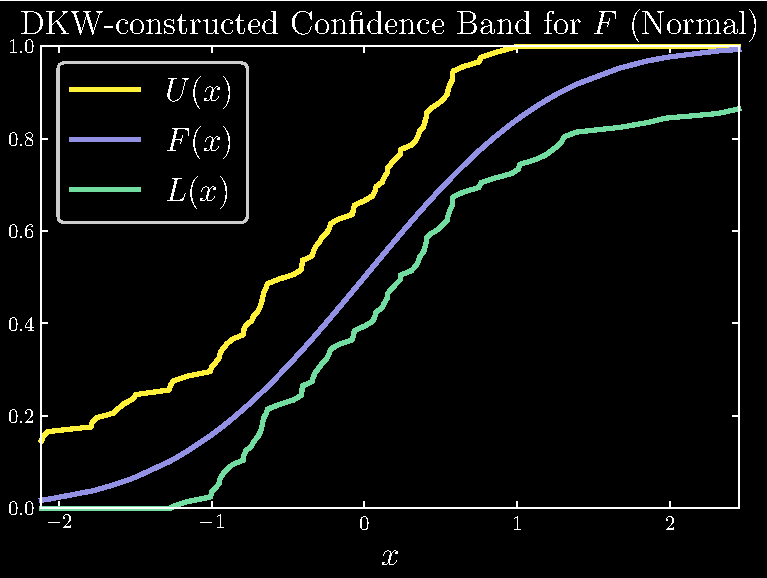
\includegraphics[width=1.0\textwidth]{chap7/chap7ex3i.eps}
\end{center}

The probability that the \textsf{CDF} \(F\) is contained in the confidence band approaches \(0.95\) for large number of iterations:

\begin{center}
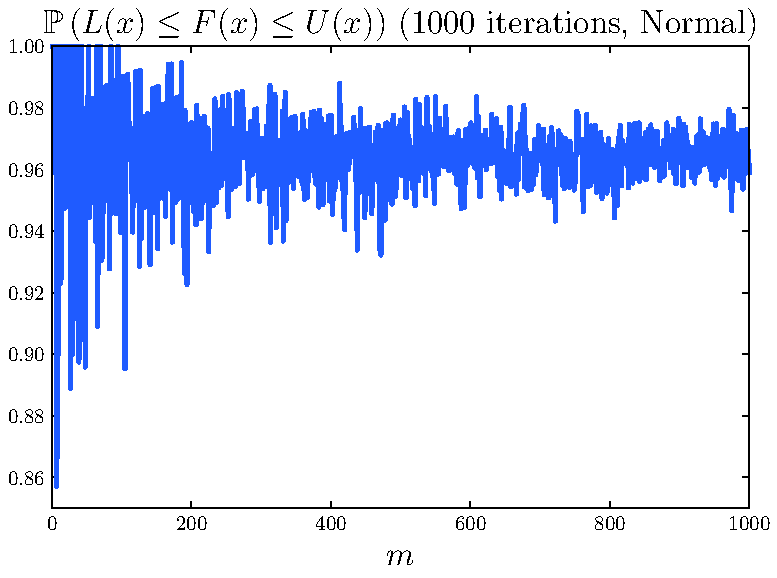
\includegraphics[width=1.0\textwidth]{chap7/chap7ex3ii.eps}
\end{center}

Repeating the same for data from a standard Cauchy distribution, we get:

\begin{python}
n = 100
alpha = 0.05
eps = np.sqrt((1/(2*n))*np.log(2/alpha))

def ecdfhat(sample):
    cdfhat = [ i/len(sample) for i in range(1, len(sample)+1)]
    return cdfhat;

def dkwintcauchy():
    dkwtest, lowerbound, upperbound = 
    	np.empty(n), np.empty(n), np.empty(n)
    sample = np.sort(np.random.standard_cauchy(n))
    ecdf = ecdfhat(sample)
    for i,j in zip(range(0, len(sample)), sample):
        lowerbound[i] = max(ecdf[i] - eps, 0)
        upperbound[i] = min(ecdf[i] + eps, 1)
        dkwtest[i] = 
		(norm.cdf(j) >= lowerbound[i]) 
		& (norm.cdf(j) <= upperbound[i])
    return dkwtest, lowerbound, upperbound, ecdf, sample;
\end{python}

\begin{center}
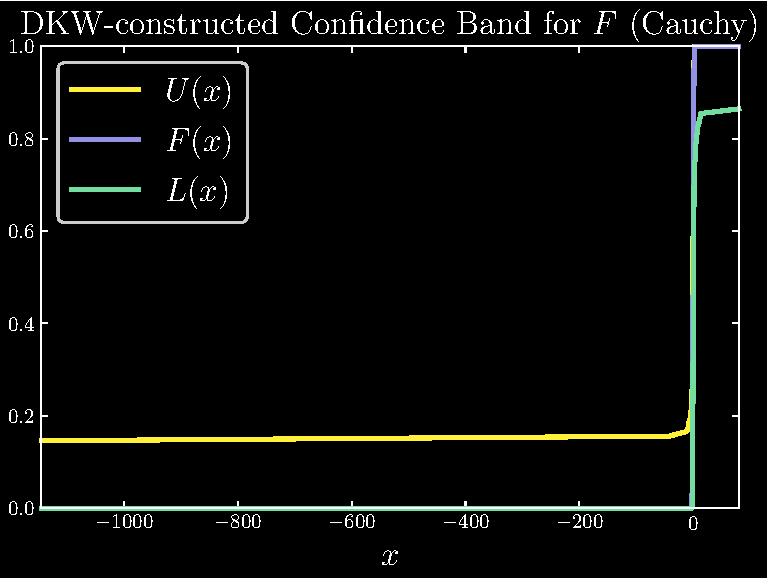
\includegraphics[width=1.0\textwidth]{chap7/chap7ex3iii.eps}
\end{center}

\begin{center}
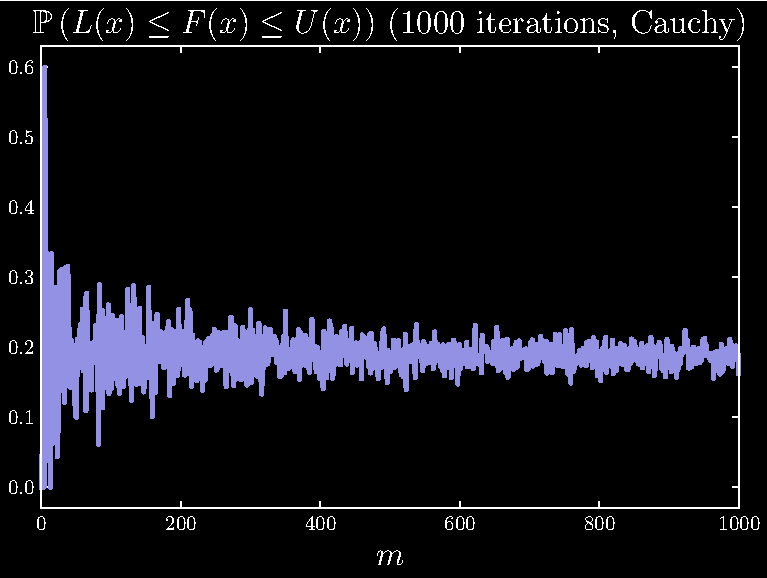
\includegraphics[width=1.0\textwidth]{chap7/chap7ex3iv.eps}
\end{center}

% QUESTION 4
\qs{7.4.4}{Let \(X_{1}, \dots, X_{n} \sim F\) and let \(\widehat{F}_{n} \left( x \right) \) be the empirical distribution function. For a fixed \(x\), use the central limit theorem to find the limiting distribution of \(\widehat{F}_{n} \left( x \right) \).}

Using Theorem 7.3 and the proof from exercise 7.4.1, by the Central Limit Theorem, we have
\[
	\widehat{F}_{n} \left( x \right) \approx N \left( F \left( x \right) , \frac{F \left( x \right) \left( 1 - F \left( x \right)  \right) }{n} \right) 
\]

\newpage
% QUESTION 5
\qs{7.4.5}{Let \(x\) and \(y\) be two distinct points. Find \( \cov\left( \widehat{F}_{n}\left( x \right) , \widehat{F}_{n} \left( y \right)  \right)\).}

By definition of covariance, we have \(\cov\left( \widehat{F}_{n} \left( x \right) , \widehat{F}_{n} \left( y \right)  \right)\) equal to:
\begin{align*}
	 & = \E\left( \left( \widehat{F}_{n}\left( x \right) - \E\left( \widehat{F}_{n}\left( x \right)  \right) \right) \left( \widehat{F}_{n}\left( y \right) - \E\left( \widehat{F}_{n}\left( y \right)  \right) \right)  \right) \\
	 & = \E\left( \left( \widehat{F}_{n}\left( x \right) - F \left( x \right)  \right) \left( \widehat{F}_{n}\left( y \right) - F \left( y \right)  \right)  \right)  \\ 
	 & = \E\left( \widehat{F}_{n}\left( x \right) \widehat{F}_{n}\left( y \right)  \right) - F \left( x \right) F \left( y \right) \\
	 & = \E\left( \frac{1}{n^{2}} \left( \sum_{i=1}^{n} I \left( X_{i} \le x \right)  \right) \left( \sum_{j=1}^{n} I \left( X_{j} \le y \right)  \right)  \right) - F \left( x \right) F \left( y \right) \\
	 & = \frac{1}{n^{2}} \E\left( \sum_{i=1}^{n} I \left( X_{i} \le x \right) I \left( X_{i} \le y \right) + \sum_{i=1}^{n} \sum_{\substack{j = 1 \\ j \neq i}}^{n} I \left( X_{i} \le x \right) I \left( X_{j} \le y \right)  \right) \\
	 & \quad - F \left( x \right) F \left( y \right) 
\end{align*}

Now, for the first term to have non-zero terms in the sum, we must have \(X_{i} \le x,y\). Since \(x,y\) are distinct, either \(x < y\) or \(y < x\). Suppose without loss of generality that \(x < y\). Then the first term resolves to
\[
	\E\left( \sum_{i=1}^{n} I \left( X_{i} \le x \right) I \left( X_{i} \le y \right)  \right) = n \Prob\left( X_{i} \le y \right) = n F \left( y \right) 
\]

For the second term, assuming independence, we have
\begin{align*}
	\E\left( \sum_{i=1}^{n} \sum_{\substack{j = 1 \\ j \neq i}}^{n} I \left( X_{i} \le x \right) I \left( X_{j} \le y \right)  \right) & = n \left( n-1 \right) \Prob\left( X_{i} \le x \right) \Prob\left( X_{j}<= y \right) \\
	 & = n \left( n-1 \right) F \left( x \right) F \left( y \right)  \\ 
\end{align*}

Combining the terms, we can conclude that the covariance is equal to
\begin{align*}
	 & = \frac{1}{n^{2}} \left( n F \left( y \right) + n \left( n - 1 \right) F \left( x \right) F \left( y \right)  \right) - F \left( x \right) F \left( y \right)  \\
	 & = \frac{F \left( y \right) + \left( n - 1 \right) F \left( x \right) F \left( y \right) - n F \left( x \right) F \left( y \right) }{n} \\ 
	 & = \boxed{\frac{F \left( y \right) \left( 1 - F \left( x \right)  \right) }{n}}
\end{align*}

% QUESTION 6
\qs{7.4.6}{Let \(X_{1}, \dots, X_{n} \sim F\) and let \(\widehat{F}\) be the empirical distribution function. Let \(a < b\) be fixed numbers and define \(\theta = T \left( F \right) = F \left( b \right) - F \left( a \right) \). Let \(\widehat{\theta} = T \left( \widehat{F}_{n} \right) = \widehat{F}_{n} \left( b \right) - \widehat{F}_{n} \left( a \right) \). Find the estimated standard error of \(\widehat{\theta}\). Find an expression for an approximate \(1 - \alpha \) confidence interval for \(\theta\).}

Using exercise 7.4.5, we can derive
\begin{align*}
	\var\left( \widehat{\theta} \right) & = \var\left( \widehat{F}_{n} \left( b \right) - \widehat{F}_{n} \left( a \right)  \right) \\
	 & = \var\left( \widehat{F}_{n} \left( b \right)  \right) + \var\left( \widehat{F}_{n} \left( a \right)  \right) + 2 \cov\left( \widehat{F}_{n} \left( b \right), \widehat{F}_{n}\left( a \right)  \right) \\
	 & = \frac{1}{n} \left( F \left( b \right) \left( 1 - F \left( b \right)  \right) + F \left( a \right) \left( 1 - F \left( a \right)  \right) + 2 F \left( b \right) \left( 1 - F \left( a \right)  \right)  \right) \\
	 & = \frac{1}{n} \left( F \left( b \right) - F \left( a \right)  \right) \left( 1 - \left( F \left( b \right) - F \left( a \right)  \right)  \right) \\
	\se \left( \widehat{\theta} \right) & = \sqrt{\var\left( \widehat{\theta} \right)} \\
	\widehat{\se } \left( \widehat{\theta} \right) & = \sqrt{\frac{1}{n} \left( \widehat{F}  \left( b \right) - \widehat{F} \left( a \right)  \right) \left( 1 - \left( \widehat{F} \left( b \right) - \widehat{F} \left( a \right)  \right)  \right)} \\
\end{align*}
The \(1 - \alpha \) confidence interval is given by
\[
	\widehat{\theta} \pm z_{\alpha /2} \widehat{\se} \left( \widehat{\theta} \right) 
\]

% QUESTION 7
\qs{7.4.7}{Data on the magnitudes of earthquakes near Fiji are available on the website for this book. Estimate the \textsf{CDF} \(F \left( x \right) \). Compute and plot a 95 percent confidence envelope for \(F\). Find an approximate 95 percent confidence interval for \(F \left( 4.9 \right) - F \left( 4.3 \right) \).}

The 95 percent confidence interval for \(F(4.9) - F(4.3)\) is \((0.495, 0.557)\).
The DKW-constructed confidence band for \(F\) is as follows:

\begin{python}
fijidata = pd.read_csv('fijiquakes.dat', delim_whitespace=True)

magdata = np.sort(fijidata['mag'])

n = len(magdata)
alpha = 0.05
eps = np.sqrt((1/(2*n))*np.log(2/alpha))

def ecdfhat(sample):
    cdfhat = [ i/len(sample) for i in range(1, len(sample)+1)]
    return cdfhat;

def dkwbounds():
    lowerbound, upperbound = 
    	np.empty(len(magdata)), 
	np.empty(len(magdata))
    ecdf = ecdfhat(magdata)
    for i in range(0, len(magdata)):
        lowerbound[i] = max(ecdf[i] - eps, 0)
        upperbound[i] = min(ecdf[i] + eps, 1)
    return lowerbound, upperbound;

# Use results of exercise 7.4.6 for confidence interval

theta = ecdf(4.9) - ecdf(4.3)
sehat = np.sqrt((1/len(magdata))*theta*(1-theta))
\end{python}

\begin{center}
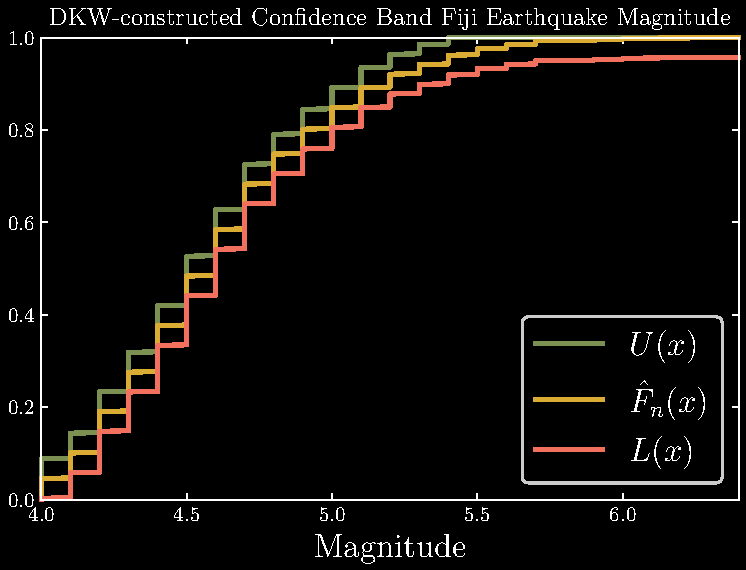
\includegraphics[width=1.0\textwidth]{chap7/chap7ex7.eps}
\end{center}

\newpage
% QUESTION 8
\qs{7.4.8}{Get the data on eruption times and waiting times between eruptions of the Old Faithful geyser from the website. Estimate the mean waiting time and give a standard error for the estimate. Also, give a 90 percent confidence interval for the mean waiting time. Now estimate the median waiting time. In the next chapter we will see how to get the standard error for the median.}

The estimated mean, standard error, 90 percent confidence interval, and median are \(70.897\), \(0.824\), \((69.537, 72.257)\), and \(76.0\), respectively.

\begin{python}
faithful = pd.read_csv('faithful.dat', delim_whitespace=True)
    
waitingdata = faithful['waiting']

waitingmean = np.mean(waitingdata)
waitingse = np.std(waitingdata, ddof=1) / np.sqrt(np.size(waitingdata))

waitingci = (round(waitingmean - 1.65*waitingse, 3), 
	     round(waitingmean + 1.65*waitingse, 3))

waitingmedian = np.median(waitingdata)
\end{python}


% QUESTION 9
\qs{7.4.9}{100 people are given a standard antibiotic to treat an infection and another 100 are given a new antibiotic. In the first group, 90 people recover; in the second group, 85 people recover. Let \(p_{1}\) be the probability of recovery under the standard treatment and let \(p_{2}\) be the probability of recovery under the new treatment. We are interested in estimating \(\theta = p_{1} - p_{2}\). Provide an estimate, standard error, an 80 percent confidence interval, and a 95 percent confidence interval for \(\theta\).}

We can model the odds of recovering as a Bernoulli variable. We estimate \(\widehat{\theta}\) as
\[
	\widehat{\theta} = \widehat{p_{1} - p_{2}} = \frac{90}{100} - \frac{85}{100} = \boxed{0.05}
\]
The estimate of the standard error is
\begin{align*}
	\widehat{\se }\left( \widehat{\theta} \right)  & = \sqrt{\frac{\widehat{p}_{1} \left( 1 - \widehat{p}_{1} \right) }{n} + \frac{\widehat{p}_{2} \left( 1 - \widehat{p}_{2} \right) }{n}} \\
	 & = \sqrt{\frac{90 / 100 \left( 1 - 90 / 100 \right) }{100} + \frac{85 / 100 \left( 1 - 85/100 \right) }{100}} \\ 
	 & \approx \boxed{0.0466}
\end{align*}

\underline{80 percent CI:} \(z_{\alpha /2} = z_{.2 / 2} = z_{0.1} \approx 1.28\)
\[
	0.05 \pm 0.0597
\]

\underline{95 percent CI:} \(z_{\alpha /2} = z_{0.05/2} = z_{0.025} \approx 1.96\)
\[
	0.05 \pm 0.0914
\]

% QUESTION 10
\qs{7.4.10}{In 1975, an experiment was conducted to see if cloud seeding produced rainfall. 26 clouds were seeded with silver nitrate and 26 were not. The decision to seed or not was made at random.

Let \(\theta\) be the difference in the mean precipitation from the two groups. Estimate \(\theta\). Estimate the standard error of the estimate and produce a 95 percent confidence interval.}

The estimates for \(\theta\), standard error, and the 95 percent confidence interval are \(277.396\), \(136.124\), and \((10.593, 544.199)\), respectively.

\begin{python}
clouds = pd.read_csv('clouds.dat', delim_whitespace=True)

unseeded = clouds['Unseeded_Clouds']
seeded = clouds['Seeded_Clouds']

diffmean = np.abs(np.mean(unseeded) - np.mean(seeded))
unseeded_se = np.std(unseeded) / np.sqrt(np.size(unseeded))
seeded_se = np.std(seeded) / np.sqrt(np.size(seeded))
diffse = np.sqrt(np.square(unseeded_se) + np.square(seeded_se))

diffci = (round(diffmean - 1.96*diffse, 3), 
	 round(diffmean + 1.96*diffse, 3))
\end{python}

\section{Chapter 8: The Bootstrap}

% QUESTION 1
\qs{8.6.1}{Consider the data in Example 8.6. Find the plug-in estimate of the correlation coefficient. Estimate the standard error using the bootstrap. Find a 95 percent confidence interval using the Normal, pivotal, and percentile methods.}

We plot the LSAT and GPA data as follows:

\begin{center}
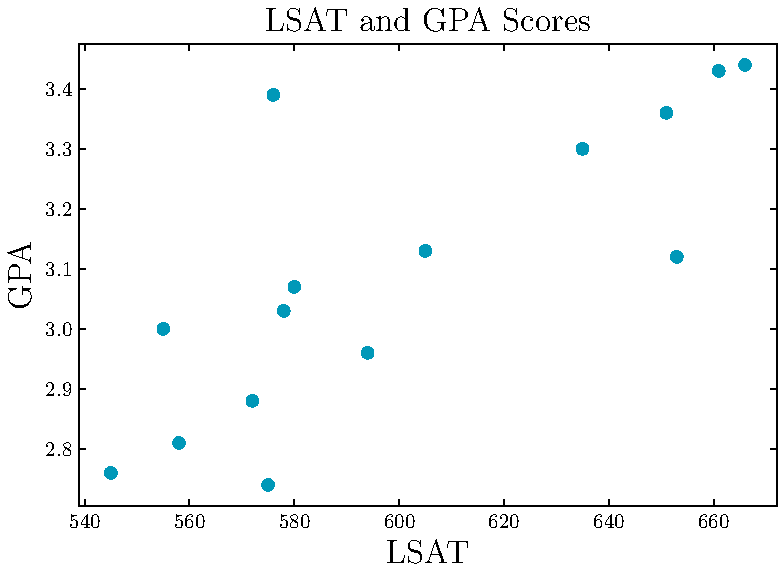
\includegraphics[width=1.0\textwidth]{chap8/chap8ex1i.eps}
\end{center}

And  calculate the plug-in estimate of the correlation as \(0.7764\). For \(B = 1000\) number of samples, we bootstrap the correlation, which has  standard error \(0.1387\). This gives us for the confidence intervals 

\renewcommand{\arraystretch}{2}
\begin{center}
\begin{tabular}{|c|c|}
	\hline
	Normal & \(\left( 0.5045, 1.0482 \right) \) \\
	\hline
	Pivotal & \(\left( 0.5944, 1.1100 \right) \) \\
	\hline
	Percentile & \(\left( 0.4428, 0.9583 \right) \) \\
	\hline
\end{tabular}
\end{center}

\begin{python}
est = pearsonr(LSAT, GPA)[0]

b = len(LSAT)
B = 1000

def bootstrap():
        bootstrapsamples = []
        for i in range(0,B):
            pairsample = choices(list(zip(LSAT,GPA)), k=b) 
            pairsample_unzip = list(zip(*pairsample))
            corrbootsample = pearsonr(pairsample_unzip[0], 
	    		     pairsample_unzip[1])[0]
            bootstrapsamples.append(corrbootsample)
        return bootstrapsamples;

sampleboot = bootstrap()

seboot = np.std(sampleboot)

normci = (est - 1.96*seboot, est + 1.96*seboot)
pivotalci = (2*est - np.quantile(sampleboot, 0.975), 
	     2*est - np.quantile(sampleboot, 0.025))
percentileci = (np.quantile(sampleboot, 0.025), 
		np.quantile(sampleboot, 0.975))
\end{python}

\begin{center}
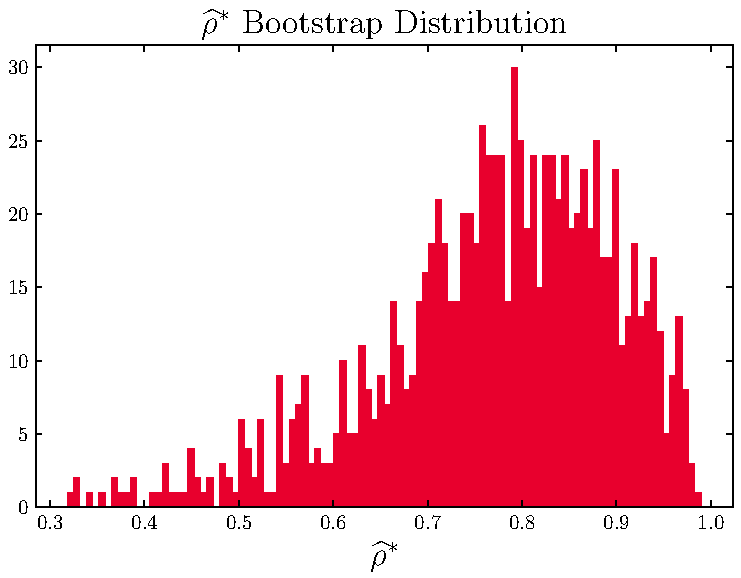
\includegraphics[width=1.0\textwidth]{chap8/chap8ex1ii.eps}
\end{center}

% QUESTION 2
\qs{8.6.2}{\textsf{(Computer Experiment.)} Conduct a simulation to compare the various bootstrap confidence interval methods. Let \(n = 50\) and let \(T \left( F \right) = \int \left( x - \mu  \right)^{3} \ dF \left( X \right) /\sigma^{3}\) be the skewness. Draw \(Y_{1}, \cdots, Y_{n} \sim N \left( 0,1 \right) \) and set \(X_{i} = e^{Y_{i}}, i = 1, \cdots, n\). Construct the three types of bootstrap 95 percent intervals for \(T \left( F \right) \) from the data \(X_{1}, \cdots, X_{n}\). Repeat this whole thing many times and estimate the true coverage of the three intervals.}

On visual inspection, the distribution of our exponentiated normal sample is extraordinarily skewed.

\begin{center}
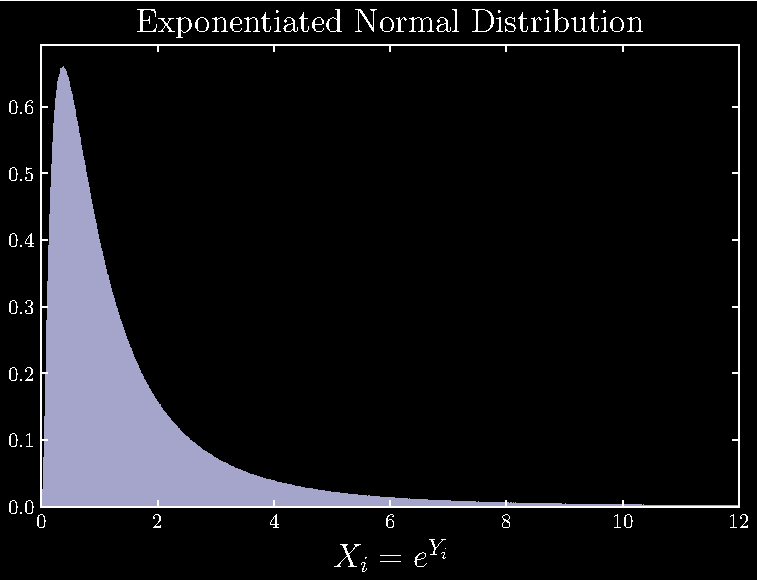
\includegraphics[width=1.0\textwidth]{chap8/chap8ex2expnormal.eps}
\end{center}

Empirically calculating the skew from a sample size of \(10^{8}\) produces values between \(6.1\) and \(6.2\). To bootstrap the skew over many iterations, as well as examining what ensues when we increase the size of the sample (from \(n = 50\)), we implement multiprocessing to conscript more CPUs to assist in the computation.

For each of the three confidence interval, we first repeat the sampling for the bootstraps \(N\) times, tabulate the standard error and construct the confidence interval, check if the true skew of distribution lies within the confidence interval, and calculate the coverage. In the second graph, we hold the number of repetitions at \(R = 100\), and instead calculate the coverage as it grows from \(N = 10\) to \(N = 1000\) samples. The relevant code is located in the chapter GitHub repo folder. 

\vspace{-3pt}
\begin{center}
\setlength{\lineskip}{-1pt}
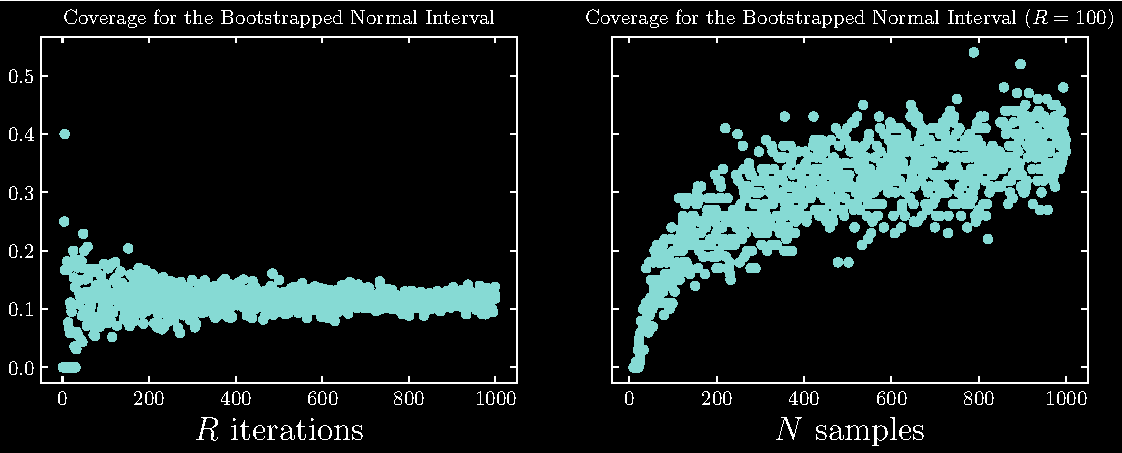
\includegraphics[width=1.0\textwidth]{chap8/chap8ex2normal.eps}
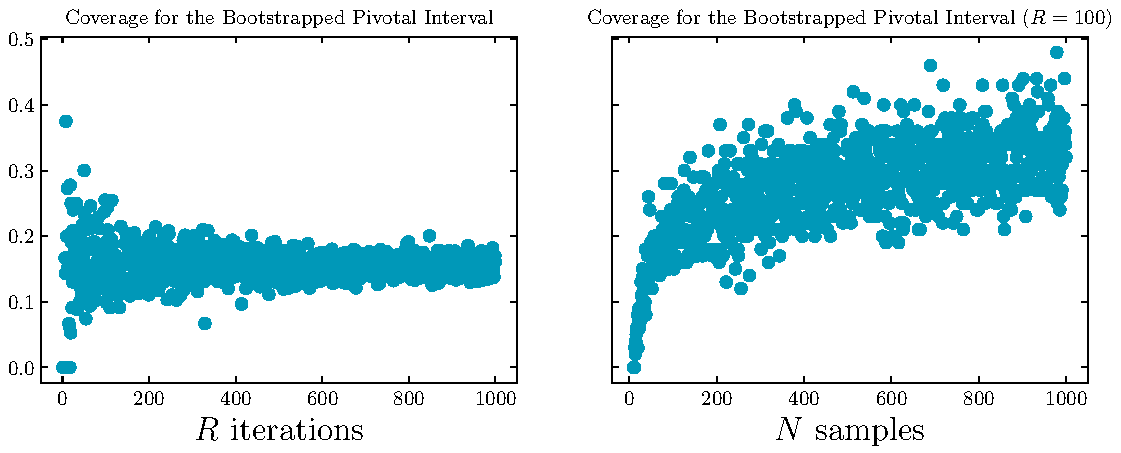
\includegraphics[width=1.0\textwidth]{chap8/chap8ex2pivotal.eps}
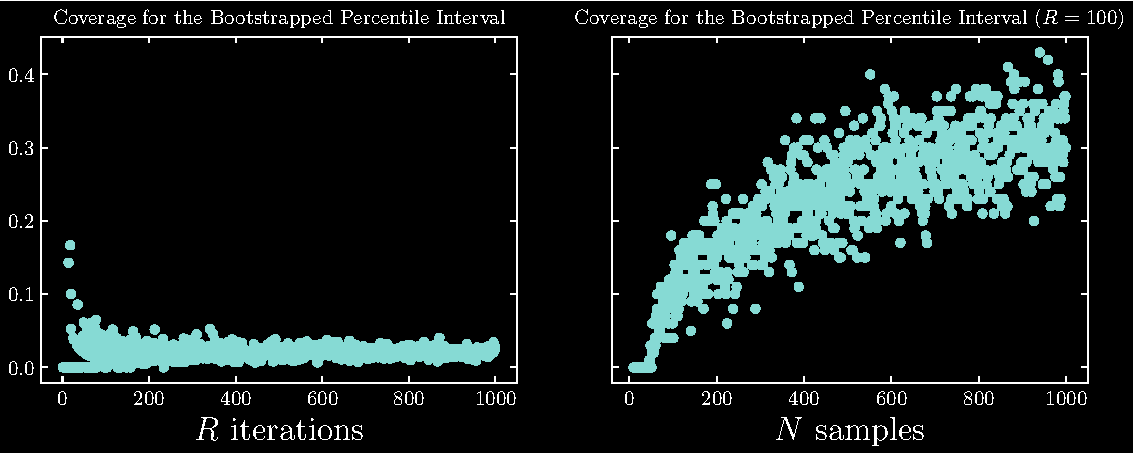
\includegraphics[width=1.0\textwidth]{chap8/chap8ex2percentile.eps}
\end{center}

% QUESTION 3
\qs{8.6.3}{Let
\[
	X_{1}, \cdots, X_{n} \sim t_{3}
\]
where \(n = 25\). Let \(\theta = T \left( F \right) = \left( q_{.75} - q_{.25} \right) / 1.34\) where \(q_{p}\) denotes the \(p^{th}\) quantile. Do a simulation to compare the coverage and length of the following confidence intervals for \(\theta\):

\begin{enumerate}[]
	\item Normal interval with standard error from the bootstrap,
	\item bootstrap percentile interval, and
	\item pivotal bootstrap interval.
\end{enumerate}}

\begin{center}
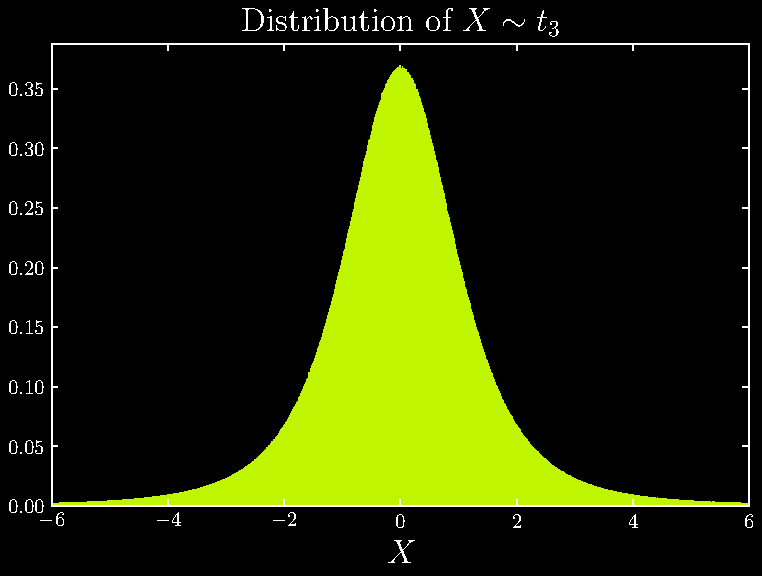
\includegraphics[width=1.0\textwidth]{chap8/chap8ex3tdistribution.eps}
\end{center}

\begin{center}
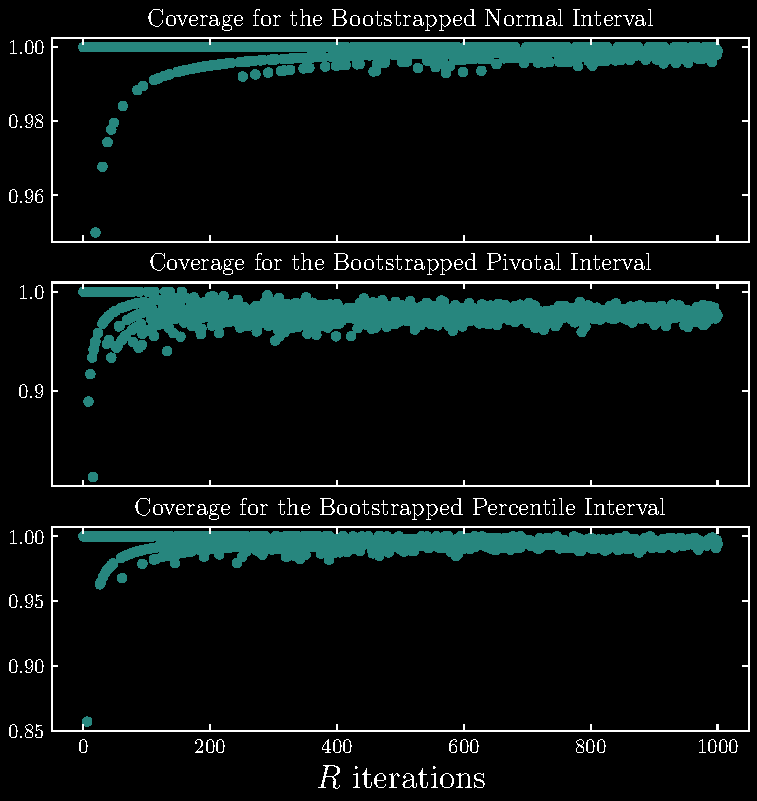
\includegraphics[width=1.0\textwidth]{chap8/chap8ex3.eps}
\end{center}

% QUESTION 4
\qs{8.6.4}{Let \(X_{1}, \dots, X_{n}\) be distinct observations (no ties). Show that there are
\[
	\binom{2n-1}{n}
\]
distinct bootstrap samples.

Hint: Imagine putting \(n\) balls into \(n\) buckets.}
\begin{proof}[Proof] 
First, let us establish some conceptual points to clarify the hint. Suppose we have three unique observations \(X_{1}, X_{2}, X_{3}\). Then we gather our bootstrap samples, obtained \textit{with} replacement. The set of all samples we can get is (using shorthand to denote that the first, second, and third digits in the sequence correspond to \(X^{*}_{1}, X^{*}_{2}, X^{*}_{3}\) equal to the first, second, or third observation):
\[
	\begin{tabular}{c c c}
		111 & 112 & 123 \\
		222 & 113 &  \\
		333 & 221 &  \\
		 & 223 &  \\
		 & 331 &  \\
		 & 332 &  \\
	\end{tabular}
\]
Now, consider 3 (identical) balls with 3 bins. One way we could place the balls in the bins is to put all of them in bin 1. Or two in bin 1, and one in bin 2. One in each bin is also an option. In other words, the combinatorial problem of how to place \(n\) balls in \(n\) bins is precisely the equivalent conundrum to resolve. The three bootstrap samples are the balls, and the specific choice of observation (\(X_{1}, X_{2}, X_{3}\)) are analogous to the choice of bin.

Developing the combinatorial theory to complete the proof is beyond the scope here.\footnote{See \textit{Combinatorics: Discrete Mathematics and its Applications}, Nicholas A. Loehr} In short, the number of ways to fit \(k\) identical balls into \(n\) bins labeled \(1, \dots, n\) is
\[
	\binom{k + n - 1}{k} = \frac{\left( k + n - 1 \right)!}{k! \left( n-1 \right)!}
\]
For \(k = n\) balls, we have
\[
	\binom{2n - 1}{n} = \frac{\left( 2n-1 \right)!}{n! \left( n-1 \right)!}
\]
\end{proof}

\end{document}
